\documentclass[PublicacaoDissOuTese,portuguese,english,LogoINPE,CCBYNC]{tdiinpe}

% \usepackage{etex}
\usepackage{makeidx}
\usepackage{graphicx}
\usepackage{multirow}
%\usepackage{caption}
\usepackage{changes}
\usepackage{algpseudocode}
\usepackage{algorithm}
\usepackage{parskip}
\usepackage{rotating}
\usepackage[graphicx]{realboxes}
\usepackage{xcolor}
\usepackage{color}
\usepackage{titlesec}
\usepackage{mathtools}
\usepackage[outline]{contour}
\usepackage{adjustbox}
\usepackage{enumitem}
\usepackage[final]{listings}
\usepackage{array}
\usepackage{forest}
\usepackage[skins]{tcolorbox}
\usepackage{enumitem}
\usepackage{longtable}
\usepackage{pdflscape}
\usepackage{pgfplotstable}
\usepackage{pgfplots}
\usepackage{pgfgantt}
\usepackage{tikzscale}
\usepackage{breakcites}
\usepackage{amsmath}
\usepackage{booktabs}
\usepackage{dirtytalk}
\usepackage{makecell}
% \usepackage{subcaption}
\usepackage{smartdiagram}
\usepackage{hyperref}
\usepackage{cleveref}
\usepackage{calligra}
\usepackage[T1]{fontenc}
\usepackage{acronym}
\usepackage{epigraph}
\usepackage{morewrites}
\usepackage{pdfrender}

\newcommand{\subfigureautorefname}{Figure}

\renewcommand{\epigraphsize}{\small}
\setlength{\epigraphwidth}{0.6\textwidth}
\renewcommand{\textflush}{flushright}
\renewcommand{\sourceflush}{flushright}
% A useful addition
\newcommand{\epitextfont}{\itshape}
\newcommand{\episourcefont}{\scshape}

\makeatletter
\newsavebox{\epi@textbox}
\newsavebox{\epi@sourcebox}
\newlength\epi@finalwidth
\renewcommand{\epigraph}[2]{%
  \vspace{\beforeepigraphskip}
  {\epigraphsize\begin{\epigraphflush}
   \epi@finalwidth=\z@
   \sbox\epi@textbox{%
     \varwidth{\epigraphwidth}
     \begin{\textflush}\epitextfont#1\end{\textflush}
     \endvarwidth
   }%
   \epi@finalwidth=\wd\epi@textbox
   \sbox\epi@sourcebox{%
     \varwidth{\epigraphwidth}
     \begin{\sourceflush}\episourcefont#2\end{\sourceflush}%
     \endvarwidth
   }%
   \ifdim\wd\epi@sourcebox>\epi@finalwidth 
     \epi@finalwidth=\wd\epi@sourcebox
   \fi
   \leavevmode\vbox{
     \hb@xt@\epi@finalwidth{\hfil\box\epi@textbox}
     \vskip1.75ex
     \hrule height \epigraphrule
     \vskip.75ex
     \hb@xt@\epi@finalwidth{\hfil\box\epi@sourcebox}
   }%
   \end{\epigraphflush}
   \vspace{\afterepigraphskip}}}
\makeatother

\makeatletter 
\renewcommand\thealgorithm{\thechapter.\arabic{algorithm}} 
\@addtoreset{algorithm}{chapter} 
\makeatother

\pgfplotsset{compat=newest}
% \usepackage{definition}

\renewcommand{\floatpagefraction}{.9}%

\setlist[itemize]{topsep=0pt,before=\leavevmode\vspace{-1.5em}}
\setlist[description]{style=nextline}

\newcommand*{\tabref}[1]{\tablename~\ref{#1}}
\newcommand*{\figref}[1]{\figurename~\ref{#1}}
\newcommand*{\secref}[1]{Section~\ref{#1} \:}
\newcommand*{\algoref}[1]{Algorithm~\ref{#1}}

\newcolumntype{L}[1]{>{\raggedright\let\newline\\\arraybackslash\hspace{0pt}}p{#1}}
\newcolumntype{C}[1]{>{\centering\let\newline\\\arraybackslash\hspace{0pt}}p{#1}}
\newcolumntype{R}[1]{>{\raggedleft\let\newline\\\arraybackslash\hspace{0pt}}p{#1}}

\newcommand{\algorithmautorefname}{Algorithm}

\setcounter{secnumdepth}{4}

\titleformat{\paragraph}
{\normalfont\normalsize\bfseries}{\theparagraph}{1em}{}
\titlespacing*{\paragraph}
{0pt}{3.25ex plus 1ex minus .2ex}{1.5ex plus .2ex}

\newganttchartelement*{mymilestone}{
mymilestone/.style={
shape=isosceles triangle,
inner sep=0pt,
draw=cyan,
top color=white,
bottom color=cyan!50
},
mymilestone incomplete/.style={
/pgfgantt/mymilestone,
draw=yellow,
bottom color=yellow!50
},
mymilestone label font=\slshape,
mymilestone left shift=0pt,
mymilestone right shift=0pt
}

\newgantttimeslotformat{stardate}{%
\def\decomposestardate##1.##2\relax{%
\def\stardateyear{##1}\def\stardateday{##2}%
}%
\decomposestardate#1\relax%
\pgfcalendardatetojulian{\stardateyear-01-01}{#2}%
\advance#2 by-1\relax%
\advance#2 by\stardateday\relax%
}

\definecolor{bblue}{rgb}{0,0,.4}
\captionsetup{font=footnotesize}

\newcommand{\specialcell}[2][c]{%
  \begin{tabular}[#1]{@{}c@{}}#2\end{tabular}}

\algnewcommand\algorithmicswitch{\textbf{switch}}
\algnewcommand\algorithmiccase{\textbf{case}}
\algnewcommand\algorithmicassert{\texttt{assert}}
\algnewcommand\Assert[1]{\State \algorithmicassert(#1)}%

\algdef{SE}[SWITCH]{Switch}{EndSwitch}[1]{\algorithmicswitch\ #1\ \algorithmicdo}{\algorithmicend\ \algorithmicswitch}
\algdef{SE}[CASE]{Case}{EndCase}[1]{\algorithmiccase\ #1}{\algorithmicend\ \algorithmiccase}

\algblockdefx[Default]{Default}{EndDefault}[1][]{\textbf{default} #1}{end default}

\algtext*{EndSwitch}
\algtext*{EndCase}
\algtext*{EndWhile}
\algtext*{EndIf}
\algtext*{EndFor}
\algtext*{EndFunction}
\algtext*{EndDefault}

\bgroup
\def\arraystretch{1.5}

\usetikzlibrary{shapes}
\usetikzlibrary{plotmarks}
\usetikzlibrary{decorations.pathmorphing,patterns}
\usetikzlibrary{calc,patterns,decorations.markings}
\usetikzlibrary{shapes,arrows,calc,intersections}
\usetikzlibrary{decorations.markings}
\usetikzlibrary{decorations.pathreplacing}
\usetikzlibrary{shapes}
\usetikzlibrary{plotmarks}
\usetikzlibrary{decorations.pathmorphing,patterns}
\usetikzlibrary{calc,patterns,decorations.markings}
\usetikzlibrary{shapes,arrows,calc,intersections}
\usetikzlibrary{decorations.markings}
\usetikzlibrary{shapes}
\usetikzlibrary{plotmarks}
\usetikzlibrary{decorations.pathmorphing,patterns}
\usetikzlibrary{calc,patterns,decorations.markings}
\usetikzlibrary{shapes,arrows,calc,intersections}
\usetikzlibrary{decorations.markings}
\usetikzlibrary{mindmap,trees}
\usetikzlibrary{shadows}
\usetikzlibrary{shapes,arrows,calc,intersections}
\usetikzlibrary{decorations.markings}
\usetikzlibrary{decorations.pathreplacing} 
\usetikzlibrary{angles,quotes}
\usetikzlibrary{decorations.markings} 
\usetikzlibrary{shapes.geometric}
\usetikzlibrary{positioning}
\usetikzlibrary{calc,patterns,decorations.pathmorphing,decorations.markings}
\usetikzlibrary{patterns}
\usetikzlibrary{pgfplots.groupplots}
\usetikzlibrary{pgfplots.statistics}
\usetikzlibrary{arrows.meta}


\tikzstyle{platform}=[fill,pattern=north east lines,draw=none,minimum width=1cm,minimum height=0.3cm]

\makeatletter
\def\underscoreusetikzlibrary{\pgfutil@ifnextchar[{\underscoreuse@tikzlibrary}{\underscoreuse@@tikzlibrary}}%}
\def\underscoreuse@tikzlibrary[#1]{\underscoreuse@@tikzlibrary{#1}}
\def\underscoreuse@@tikzlibrary#1{%
  \edef\pgf@list{#1}%
  \pgfutil@for\pgf@temp:=\pgf@list\do{%
	\expandafter\pgfkeys@spdef\expandafter\pgf@temp\expandafter{\pgf@temp}%
	\ifx\pgf@temp\pgfutil@empty
	\else
		\expandafter\ifx\csname tikz@library@\pgf@temp @loaded\endcsname\relax%
		  \expandafter\global\expandafter\let\csname tikz@library@\pgf@temp @loaded\endcsname=\pgfutil@empty%
		  \expandafter\edef\csname tikz@library@#1@atcode\endcsname{\the\catcode`\@}
		  \expandafter\edef\csname tikz@library@#1@barcode\endcsname{\the\catcode`\|}
		  \catcode`\@=11
		  \catcode`\|=12
		  \input tikzlibrary\pgf@temp_code.tex
		  \catcode`\@=\csname tikz@library@#1@atcode\endcsname
		  \catcode`\|=\csname tikz@library@#1@barcode\endcsname
		\fi%
	\fi
  }%
}
\makeatother
\underscoreusetikzlibrary{mec}

\contourlength{1pt}

\renewcommand{\arraystretch}{0.9}

\tikzstyle{startstop} = [rectangle, rounded corners, minimum width=3cm, minimum height=1cm,text centered, draw=black]
\tikzstyle{io} = [trapezium, trapezium left angle=70, trapezium right angle=110, minimum width=2cm, minimum height=1cm, text centered, draw=black]
\tikzstyle{process} = [rectangle, minimum width=3cm, minimum height=1cm, text centered, draw=black]
\tikzstyle{decision} = [diamond, minimum width=3cm, minimum height=1cm, text centered, draw=black, aspect=2.5]
\tikzstyle{arrow} = [thick,->,>=stealth]
\definecolor{myyellow}{RGB}{254,241,24}
\definecolor{myorange}{RGB}{234,125,1}

\def\proton(#1,#2){%
    \fill[ball color=yellow] (#1,#2) circle (10pt);
}
\def\neutron(#1,#2){%
    \fill[ball color=blue] (#1:#2) circle (10pt);
}
\def\neutronrejeited(#1,#2){%
    \fill[ball color=blue,fill opacity=.4,draw,densely dotted] (#1:#2) circle (10pt);
}
\def\electron(#1,#2){%
    \fill[ball color=green!30] (#1:#2) circle (10pt);
}

\tikzset{->-/.style={decoration={
  markings,
  mark=at position #1 with {\arrow{latex}}},postaction={decorate}}
}

\theoremstyle{definition}
\newtheorem{definition}{Definition}[chapter]
% \newenvironment{definition}
%   {\pushQED{\qed}\renewcommand{\qedsymbol}{$\triangle$}\examplex}
%   {\popQED\endexamplex}
\providecommand*\definitionautorefname{Definition}

\def\myrad{2cm}
\def\myang{30}

\pgfdeclarepatternformonly{south west lines}{\pgfqpoint{-0pt}{-0pt}}{\pgfqpoint{3pt}{3pt}}{\pgfqpoint{3pt}{3pt}}{
        \pgfsetlinewidth{0.4pt}
        \pgfpathmoveto{\pgfqpoint{0pt}{0pt}}
        \pgfpathlineto{\pgfqpoint{3pt}{3pt}}
        \pgfpathmoveto{\pgfqpoint{2.8pt}{-.2pt}}
        \pgfpathlineto{\pgfqpoint{3.2pt}{.2pt}}
        \pgfpathmoveto{\pgfqpoint{-.2pt}{2.8pt}}
        \pgfpathlineto{\pgfqpoint{.2pt}{3.2pt}}
        \pgfusepath{stroke}}
        
\newcommand{\R}{\mathbb{R}}


\definecolor{armygreen}{rgb}{0.29, 0.33, 0.13}
\definecolor{oucrimsonred}{rgb}{0.6, 0.0, 0.0}
\definecolor{yaleblue}{rgb}{0.06, 0.3, 0.57}
\definecolor{sandstorm}{rgb}{0.93, 0.84, 0.25}
\definecolor{vegasgold}{rgb}{0.77, 0.7, 0.35}

\pgfplotsset{compat=1.11,
    /pgfplots/ybar legend/.style={
    /pgfplots/legend image code/.code={%
       \draw[##1,/tikz/.cd,yshift=-0.25em]
        (0cm,0cm) rectangle (3pt,0.8em);},
   },
}

\makeatletter

% define a macro \Autoref to allow multiple references to be passed to \autoref
\newcommand\Autoref[1]{\@first@ref#1,@}
\def\@throw@dot#1.#2@{#1}% discard everything after the dot
\def\@set@refname#1{%    % set \@refname to autoefname+s using \getrefbykeydefault
    \edef\@tmp{\getrefbykeydefault{#1}{anchor}{}}%
    \def\@refname{\@nameuse{\expandafter\@throw@dot\@tmp.@autorefname}s}%
}
\def\@first@ref#1,#2{%
  \ifx#2@\autoref{#1}\let\@nextref\@gobble% only one ref, revert to normal \autoref
  \else%
    \@set@refname{#1}%  set \@refname to autoref name
    \@refname~\ref{#1}% add autoefname and first reference
    \let\@nextref\@next@ref% push processing to \@next@ref
  \fi%
  \@nextref#2%
}
\def\@next@ref#1,#2{%
   \ifx#2@ and~\ref{#1}\let\@nextref\@gobble% at end: print and+\ref and stop
   \else, \ref{#1}% print  ,+\ref and continue
   \fi%
   \@nextref#2%
}

\makeatother

\newcommand*{\fullref}[1]{\hyperref[{#1}]{\Cref*{#1} \nameref*{#1}}} % One single link

\makeatletter
\AtBeginDocument{%
  \let\l@algorithm\l@figure%
  \let\listofalgorithms\listoffigures% Copy \listoffigures
  \let\@cftmakeloatitle\@cftmakeloftitle% Copy LoF title
  % Update LoA-related macros
  \patchcmd{\listofalgorithms}{\@cftmakeloftitle}{\@cftmakeloatitle}{}{}%
  \patchcmd{\listofalgorithms}{\@starttoc{lof}}{\@starttoc{loa}}{}{}%
  \patchcmd{\@cftmakeloatitle}{\listfigurename}{\listalgorithmname}{}{}%
  % Add per-chapter LoA space (similar to LoF)
  \patchcmd{\@chapter}{\addtocontents}{%
    \addtocontents{loa}{\protect\addvspace{10\p@}}%
    \addtocontents}{}{}%
}

\makeatother

%\watermark{Revisão No. ##}

\usepackage{rotating}
\usepackage{dsfont}
\usepackage{comment}

%%%%%%%%%%%%%%%%%%%CAPA%%%%%%%%%%%%%%%%%%%%%%%%%%%%%%%%
%\serieinpe{INPE-NNNNN-TDI/NNNN} %% n\~{a}o mais usado

\titulo{Vibration-based damage identification using hybrid metaheuristics and a hierarchical approach}
\title{Identificação de danos baseada em vibração usando algoritmos meta-heurísticos híbridos e uma abordagem hierárquica} %% 
\author{Reynier Hern\'andez Torres} %% coloque o nome do(s) autor(es)
\descriccao{Doctoral Thesis in Applied Computing (CAP) guided by \mbox{Dr. Haroldo F. de Campos Velho} and \mbox{Dr. Leonardo D. Chiwiacowsky}}
\repositorio{aa/bb/cc/dd} %% reposit\'{o}rio onde est\'a depositado este documento - na omiss\~ao, ser\'a preenchido pelo SID
\tipoDaPublicacao{TDI}	%% tipo da publica\c{c}\~ao (NTC, RPQ, PRP, MAN, PUD, TDI, TAE e PRE) na aus\^encia do número de s\'erie INPE, caso contr\'ario deixar vazio
\IBI{xx/yy} %% IBI (exemplo: J8LNKAN8PW/36CT2G2) quando existir, caso contr\'ario o nome do reposit\'{o}rio onde est\'a depositado o documento

\date{2017}%ano da publicaç\~{a}o

%%%%%%%%%%%%%%%%%%%%%%%%%%VERSO DA CAPA%%%%%%%%%%%%%%%%%%%%%%%%%%%%%%%%%%%%%%%%%%%%%%%
\tituloverso{\vspace{-0.9cm}\textbf{\PublicadoPor:}}
\descriccaoverso{Instituto Nacional de Pesquisas Espaciais - INPE\\
Gabinete do Diretor (GB)\\
Serviço de Informaç\~{a}o e Documentaç\~{a}o (SID)\\
Caixa Postal 515 - CEP 12.245-970\\
S\~{a}o Jos\'{e} dos Campos - SP - Brasil\\
Tel.:(012) 3945-6923/6921\\
Fax: (012) 3945-6919\\
E-mail: {\url{pubtc@sid.inpe.br}}
}

\descriccaoversoA{\textbf{\ConselhoDeEditoracao:}\\
\textbf{\Presidente:}\\
Marciana Leite Ribeiro - Serviço de Informaç\~{a}o e Documentaç\~{a}o (SID)\\
\textbf{\Membros:}\\
Dr. Gerald Jean Francis Banon - Coordenaç\~{a}o Observaç\~{a}o da Terra (OBT)\\
Dr. Amauri Silva Montes - Coordenaç\~{a}o Engenharia e Tecnologia Espaciais (ETE)\\
Dr. Andr\'{e} de Castro Milone - Coordenaç\~{a}o Ci\^{e}ncias Espaciais e Atmosf\'{e}ricas (CEA)\\
Dr. Joaquim Jos\'{e} Barroso de Castro -  Centro de Tecnologias Espaciais (CTE)\\
Dr. Manoel Alonso Gan - Centro de Previs\~{a}o de Tempo e Estudos Clim\'{a}ticos (CPT)\\
Drª Maria do Carmo de Andrade Nono - Conselho de P\'{o}s-Graduaç\~{a}o\\
Dr. Pl\'{i}nio Carlos Alval\'{a} - Centro de Ci\^{e}ncia do Sistema Terrestre (CST)\\
\textbf{\BibliotecaDigital:}\\
Dr. Gerald Jean Francis Banon - Coordenaç\~{a}o de Observaç\~{a}o da Terra (OBT)\\
Clayton Martins Pereira - Serviço de Informaç\~{a}o e Documentaç\~{a}o (SID)\\
%Jefferson Andrade Ancelmo - Serviço de Informaç\~{a}o e Documentaç\~{a}o (SID)\\
%Simone A. Del-Ducca Barbedo - Serviço de Informaç\~{a}o e Documentaç\~{a}o (SID)\\
%Deicy Farabello - Centro de Previs\~{a}o de Tempo  e Estudos Clim\'{a}ticos (CPT)\\
\textbf{\RevisaoNormalizacaoDocumentaria:}\\
Simone Ang\'{e}lica Del Ducca Barbedo - Serviço de Informaç\~{a}o e Documentaç\~{a}o (SID) \\
%Maril\'{u}cia Santos Melo Cid - Serviço de Informaç\~{a}o e Documentaç\~{a}o (SID)\\
Yolanda Ribeiro da Silva Souza - Serviço de Informaç\~{a}o e Documentaç\~{a}o (SID)\\
\textbf{\EditoracaoEletronica:}\\
Marcelo de Castro Pazos - Serviço de Informaç\~{a}o e Documentaç\~{a}o (SID)\\
Andr\'{e} Luis Dias Fernandes - Serviço de Informaç\~{a}o e Documentaç\~{a}o (SID)\\
}

%%%%%%%%%%%%%%%%%%%FOLHA DE ROSTO

%%%%%%%%%%%%%%%FICHA CATALOGRÁFICA
%% NÃO PREENCHER - SERÁ PREENCHIDO PELO SID

\cutterFICHAC{Cutter}
\autorUltimoNomeFICHAC{Hern\'andez Torres, Reynier} %% exemplo: Fuckner, Marcus Andr\'{e}
\autorAbreviadoFICHAC {} %% N\~{a}o usado - deixar vazio
\tituloFICHAC{Vibration-based damage identification using hybrid metaheuristics and a hierarchical approach}
\instituicaosigla{INPE}
\instituicaocidade{S\~{a}o Jos\'{e} dos Campos}
\paginasFICHAC{\pageref{numeroDePáginasDoPretexto} + \pageref{LastPage}} %% n\'{u}mero total de p\'{a}ginas
%\serieinpe{INPE-00000-TDI/0000} %% n\~{a}o mais usado
\palavraschaveFICHAC{1.~Palavra chave. 2.~Palavra chave 3.~Palavra chave. 4.~Palavra chave. 5.~Palavra chave  I.~\mbox{T\'{i}tulo}.} %% recomenda-se pelo menos 5 palavras-chaves - \mbox{} \'{e} para evitar hifenizaç\~{a}o 
\numeroCDUFICHAC{000.000} %% n\'{u}mero do CDU 

% Nota da ficha (para TD)
\tipoTD{Thesis} % Dissertaç\~{a}o ou Tese
\cursoFA{Doctorate in Applied Computing}
\instituicaoDefesa{Instituto Nacional de Pesquisas Espaciais}
\anoDefesa{2017} % ano de defesa 
\nomeAtributoOrientadorFICHAC{Advisors}	% pode ser: Orientador, Orientadora ou Orientadores
\valorAtributoOrientadorFICHAC{Dr. Haroldo F. de Campos Velho, Dr. Leonardo D. Chiwiacowsky} % nome(s) completo(s)

%%%%%%%%%%%%%%%FOLHA DE APROVAÇAO PELA BANCA EXAMINADORA
\tituloFA{\textbf{ATENÇÃO! A FOLHA DE APROVAÇÃO SERÁ INCLUIDA POSTERIORMENTE.}}
%\cursoFA{\textbf{}}
\candidatoOUcandidataFA{}
\dataAprovacaoFA{}
\membroA{}{}{}
\membroB{}{}{}
\membroC{}{}{}
\membroD{}{}{}
\membroE{}{}{}
\membroF{}{}{}
\membroG{}{}{}
\ifpdf

%%%%%%%%%%%%%%NÍVEL DE COMPRESSÃO {0 -- 9}
\pdfcompresslevel 9
\fi
%%% define em 80% a largura das figuras %%%
\newlength{\mylenfig} 
\setlength{\mylenfig}{0.8\textwidth}
%%%%%%%%%%%%%%%%%%%%%%%%%%%%%%%%%%%%%%%%%%%

%%%%%%%%%%%%%%COMANDOS PESSOAIS
\newcommand{\vetor}[1]{\mathit{\mathbf{#1}}}
\makeindex

\begin{document}

%\marcaRegistrada{}	% comando opcional usado para informar abaixo da ficha catalográfica sobre marca registrada

\maketitle

\begin{epigrafe}

\hypertarget{estilo:epigrafe}{}

{
\centering
\epigraph{\large Science is knowledge which we understand so well that we can teach it to a computer; and if we don't fully understand something, it is an art to deal with it.}{\textit{\large Donald E. Knuth} \\ ``Computer Programming as an Art'', 1974}
}

\end{epigrafe}
 %% Opcional
%%%%%%%%%%%%%%%%%%%%%%%%%%%%%%%%%%%%%%%%%%%%%%%%%%%%%%%%%%%%%%%%%%%%%%%%%%%%%%%%
% Dedicatória %% opcional

\begin{dedicatoria} %% insira sua dedicatória abaixo; estilo livre

\hypertarget{estilo:dedicatoria}{} %% uso para este Guia

\newcommand{\mytext}{A mis padres \textbf{Consuelo} y \textbf{Juan}}

\vspace*{\fill}
\calligra\Large \mytext
\vspace*{\fill}

\end{dedicatoria} %% Opcional
% %%%%%%%%%%%%%%%%%%%%%%%%%%%%%%%%%%%%%%%%%%%%%%%%%%%%%%%%%%%%%%%%%%%%%%%%%%%%%%%%
% AGRADECIMENTOS %% opcional

\begin{agradecimentos}  %% insira abaixo seus agradecimentos

\hypertarget{estilo:agradecimentos}{} %% uso para este Guia
Agradecimentos
\end{agradecimentos}


 %% Opcional
%%%%%%%%%%%%%%%%%%%%%%%%%%%%%%%%%%%%%%%%%%%%%%%%%%%%%%%%%%%%%%%%%%%%%%%%%%%%%%%%
% ABSTRACT
\begin{resumo}

\hypertarget{estilo:resumo}{}

A hybrid metaheuristic combing the Multi-Particle Collision Algorithm (MPCA) with the Hooke-Jeeves (HJ) method is applied to identify the structural damage. A new version of the MPCA is formulated with the rotation-based learning mechanism to the exploration search. The inverse problem of damage identification is formulated as an optimization problem assuming the displacement time history as experimental data. The objective function is the square difference between the measured displacement and the displacement calculated by the forward model. The approach was tested on a cantilevered beam structure. Time-invariant damages were assumed to generate the synthetic displacement data. Noiseless and noisy data were considered. Finite element method was used for solving the direct problem.  The comparison between standard MPCA-HJ and the new version of the hybrid method is reported. The use of these hybrid algorithms allows to obtain good estimations using a full set of data, or using a reduced dataset with a low level of noise in data.


The hybrid metaheuristic Rotation-Based Sampling Multi-Particle Collision Algorithm with Hooke-Jeeves (RBSMPCA-HJ) is applied for damage identification in the Kabe's problem. Multi-Particle Collision Algorithm is a metaheuristic algorithm that performs a search on the solution space. With the addition of the Rotation-Based Sampling mechanism to the exploration search, a major area of the solution space has a chance to be visited. The Hooke-Jeeves is a direct search method that exploits the best solution found by the RBSMPCA, allowing to achieve better solutions. Experimental data were generated in silico, using time-invariant damages. Experiments with noiseless and noisy data were carried out. Good estimations of damage location and severity are achieved.

\palavraschave{%
	\palavrachave{vibration-based damage identification}%
	\palavrachave{nastran}%
	\palavrachave{inverse problem}%
	\palavrachave{multi-particle collision algorithm}%
	\palavrachave{qG method}%
	\palavrachave{hooke-jeeves}%
}
 
\end{resumo}

\begin{abstract}

\selectlanguage{portuguese}

\hypertarget{estilo:abstract}{}

Resumo em português

\keywords{%
	\palavrachave{Identificação de danos baseada em vibração}%
	\palavrachave{nastran}%
	\palavrachave{problema inverso}%
	\palavrachave{Algoritmo de colissão de multiplas partículas}%
	\palavrachave{método qG}%
	\palavrachave{hooke-jeeves}%
}

\selectlanguage{english}

\end{abstract} %% obrigatório

\cleardoublepage
\phantomsection
\pdfbookmark[0]{\listfigurename}{listfigurename}
\includeListaFiguras

\phantomsection
\pdfbookmark[0]{\listtablename}{listtablename}
\includeListaTabelas

\phantomsection
\pdfbookmark[0]{LIST OF ALGORITHMS}{listalgorithmname}
\includeListaAlgoritmos

\phantomsection
\pdfbookmark[0]{\nomeabreviaturasesiglas}{nomeabreviaturasesiglas}
\begin{abreviaturasesiglas}

%% sigla (separador: &--&) significado (quebra de linha: \\)
\\
ABC &--& Artificial Bee Colony \\
ACO &--& Ant Colony Optimization\\
AE &--& Acoustic Emission \\
AIS &--& Artificial Immune Systems \\
AU &--& Acousto-ultrasonic \\
BBC &--& Big Bang-Big Crunch \\
BBO &--& Biogeography-based Optimization \\
BFO &--& Bacterial Foraging Optimization \\
BMO &--& Bird Mating Optimizer \\
BVID &--& Barely Visible Impact Damage \\
CA &--& Cultural Algorithms \\
CAE &--& Computer-Aided Engineering \\
CBERS &--& China-Brazil Earth Resources Satellite \\
CB-MPCA &--& Center-based Sampling MPCA \\
CM &--& Condition Monitoring \\
CoFE &--& Compatible Finite Elements \\
CPU &--& Central Processing Unit \\
DE &--& Differential Evolution \\
DOF &--& Degrees of freedom \\
DP &--& Damage Prognosis \\
EMI &--& Electromechanical Impedance \\
EMBRAER &--& \textit{Empresa Brasileira de Aeron\'autica} \\
EP &--& Evolutionary Programming \\
ES &--& Evolution Strategies \\
FEA &--& Finite Element Analysis \\
FEM &--& Finite Element Method \\
GA &--& Genetic Algorithm \\
GH &--& Greedy Heuristic \\
GP &--& Genetic Programming \\
HJ &--& Hooke-Jeeves \\
HS &--& Harmony Search \\
ILS &--& Iterated Local Search \\
INPE &--& \textit{Instituto Nacional de Pesquisas Espaciais} \\
IP &--& Inverse Problem \\
ISS &--& International Space Station \\
IWS &--& Intelligent Water Drops \\
KMA &--& Kabe's Stiffness Matrix Adjustement \\
LS &--& Local Search \\
MA &--& Memetic Algorithm \\
MPCA &--& Multi-Particle Collision Algorithm \\
MSC &--& MacNeal-Schendler Corporation \\
NASA  &--& National Aeronautics and Space Administration \\
NASTRAN &--& NASA Structural Analysis System  \\
NDE &--& Non-Destructuve Damage Evaluation \\
NDD &--& Non-Destructuve Damage Detection \\
NM &--& Nelder-Mead algorithm \\
OBL &--& Opposition Based Learning \\
O-MPCA &--& Oppositional MPCA \\
PCA &--& Particle Collision Algorithm \\
PSO &--& Particle Swarm Optimization \\
$q$G &--& $q$-Gradient \\
QO-MPCA &--& Quasi-Oppositional MPCA \\
QR-MPCA &--& Quasi-Reflective MPCA \\
RB &--& Rotation-based Learning \\
RBS &--& Rotation-based Sampling \\
SA &--& Simulated Annealing \\
SCD &--& Data Collection Satellite \\
SDI &--& Structural Damage Identification \\
SHM &--& Structural Health Monitoring \\
SPC &--& Statistical Process Control \\
SV &--& Structural Vibration \\
TS &--& Tabu Search \\
UT &--& Ultrasonic Testing \\
VDI &--& Vibration-based Damage Identification \\

\end{abreviaturasesiglas}


\phantomsection
\pdfbookmark[0]{\listsimbname}{listsimbname}
%%%%%%%%%%%%%%%%%%%%%%%%%%%%%%%%%%%%%%%%%%%%%%%%%%%%%%%%%%%%%%%%%%%%%%%%%%%%%%%%
% simbolos

\begin{simbolos}

%% o comando: \hypertarget{estilo:simbolos}{} abaixo é de uso para este Guia
%% e pode ser retirado

\hypertarget{estilo:simbolos}{}
\\
\multicolumn{3}{l}{\textit{Latin symbols}} \\
$A$ &--& Cross-sectional area \\
$c$ &--& $\cos\theta$ \\
$C$ &--& Viscous damping \\
$D$ &--& number of decision variables \\
$e$ &--& Residual \\
$E$ &--& Young's modulus (modulus of elasticity)\\
$f$ &--& Force \\
$F$ &--& External force \\
$g(\cdot)$ &--& Inequality constraint \\
$h(\cdot)$ &--& Equality constraint \\
$h$ &--& Step size (HJ) \\
$J(\cdot)$ &--& Objective function \\
$k$ &--& Stiffness vector \\
$K$ &--& Stiffness matrix \\
$\ell$ &--& Lenght \\
$L$ &--& Largest distance within the search space \\
$M$ &--& Mass matrix \\
$n_m$ &--& Number of measured displacements \\
$N$ &--& Modal force \\
$N_{FE}$ &--& Number of function evaluations\\
$N_{particles}$ &--& Number of particles (MPCA) \\
$N_{processor}$ &--& Number of processors (MPCA) \\
$\mathcal{N}$ &--& Random number (normal distribution) \\
$p_s$ &--& Scattering probability \\
$q$ &--& $q$ parameter ($q$G) \\
$R$ &--& Random number (uniform distribution)\\
$\R$ &--& Real number \\
$s$ &--& $\sin\theta$ \\
$t$ &--& Time \\
$T$ &--& Transformation matrix \\
$u$ &--& Displacement vector \\
$v$ &--& Search direction ($q$G) \\
$V$ &--& Search direction matrix (HJ) \\
$w$ &--& Internal forces vector\\
$x, y, z$ &--& Coordinate system axes\\
\\
\multicolumn{3}{l}{\textit{Roman symbols}}\\
$\alpha$  &--& Step length \\
$\beta$ &--& Deflection angle (RB) \\
$\beta$ &--& Reduction factor ($q$G) \\
$\delta$ &--& Deformation\\
$\epsilon$ &--& Axial strain\\
$\zeta$ &--& Modal damping ratio \\
$\theta$ &--& Rotation vector\\
$\Theta^d$ &--& Damage parameters \\
$\Theta^e$ &--& Environmental and operational conditions \\
$\xi$ &--& Modal coordinate \\
$\rho$ &--& Density\\
$\rho$ &--& Reduction factor of the step (HJ)\\
$\sigma$ &--& Axial stress\\
$\sigma$ &--& Standard deviation \\
$\tau$ &--& Delay\\
$\Phi$ &--& Modal vector\\
$\Phi_w$ &--& Transformation matrix\\
$\omega$ &--& Modal frequency \\
\\
\multicolumn{3}{l}{\textit{Subscripts}}\\
$(\cdot)_{cb}$ &--& Center-based sampling \\
$(\cdot)_d$ &--& Dimension $d$ \\
$(\cdot)_i$ &--& Processor $i$ \\
$(\cdot)_j$ &--& Particle $j$ \\
$(\cdot)_m$ &--& Measurement $m$ \\
$(\cdot)_{min}$ &--& Minimum value \\
$(\cdot)_o$ &--& Opposite \\
$(\cdot)_q$ &--& Referent to $q$-gradient \\
$(\cdot)_{qo}$ &--& Quasi-opposite \\
$(\cdot)_{qr}$ &--& Quasi-reflected \\
$(\cdot)_r$ &--& Rotated \\
$(\cdot)_{rbs}$ &--& Rotation-based sampling \\
$(\cdot)_0$ &--& Initial \\
\\
\multicolumn{3}{l}{\textit{Superscripts}}\\
$(\cdot)^b$ &--& Best solution \\
$(\cdot)^c$ &--& Current solution (HJ)\\
$(\cdot)^d$ &--& Damaged \\
$(\cdot)^i$ &--& Integral \\
$(\cdot)^{inf}$ &--& Inferior limit \\
$(\cdot)^l$ &--& Lower bound \\
$(\cdot)^{mod}$ &--& Data obtained from the structural model\\
$(\cdot)^n$ &--& New solution (MPCA)\\
$(\cdot)^{obs}$ &--& Measured or observed data\\
$(\cdot)^{sup}$ &--& Superior limit \\
$(\cdot)^u$ &--& Upper bound \\
$(\cdot)^*$ &--& Globally optimal \\
$(\cdot)^\prime$ &--& Locally optimal \\
$(\cdot)^\Diamond$ &--& Best solution overall (MPCA) \\
$(\cdot)^\star$ &--& Perturbed solution (MPCA) \\
$(\cdot)^\S$ &--& Exploitaited solution (MPCA) \\
$(\cdot)^{\circ}$ &--& Pattern point (HJ) \\
\\
\multicolumn{3}{l}{\textit{Others}}\\
$\dot{\,}$ &--& First derivative \\
$\ddot{\,}$ &--& Second derivative \\
$\tilde{\,}$ &--& Optimal solution \\
$\hat{\,}$ &--& Noise added to the data\\
$\nabla$ &--& Gradient \\
$\| (\cdot) \|$ &--& Norm\\
\end{simbolos}



\includeSumario.
\inicioIntroducao

\chapter{Introduction}
\label{chp:1}
\epigraph{Research is what I'm doing when I don't know what I'm doing.}{Wernher von Braun}

The Brazilian aerospace industry is strongly represented in the world by Embraer (in portuguese \textit{Empresa Brasileira de Aeron\'autica}). This company, through its aircraft, is one of the leading exporters of Brazil, with the highest added value product. Examples of aircraft produced by Embraer are the executive Legacy 600 (\autoref{fig:e600}), the military Super Tucano (\autoref{fig:etucano}) and the commercial E-jets  (\autoref{fig:ejets}).

\begin{figure}[H]%
\caption[Embraer aircrafts]{Embraer aircrafts:
\subref{fig:e600} Legacy 600;
\subref{fig:etucano} Super Tucano;
\subref{fig:ejets} E-jets}%
\label{fig:aircrafts}%
\begin{center}
\subfigure[][]{%
\label{fig:e600}%
\begin{minipage}{0.45\textwidth}
\centering
\includegraphics[width=0.8\linewidth]{figs/Embraer_Legacy_600}%
\end{minipage}}
%
\subfigure[][]{%
\label{fig:etucano}%
\begin{minipage}{0.45\textwidth}
\centering
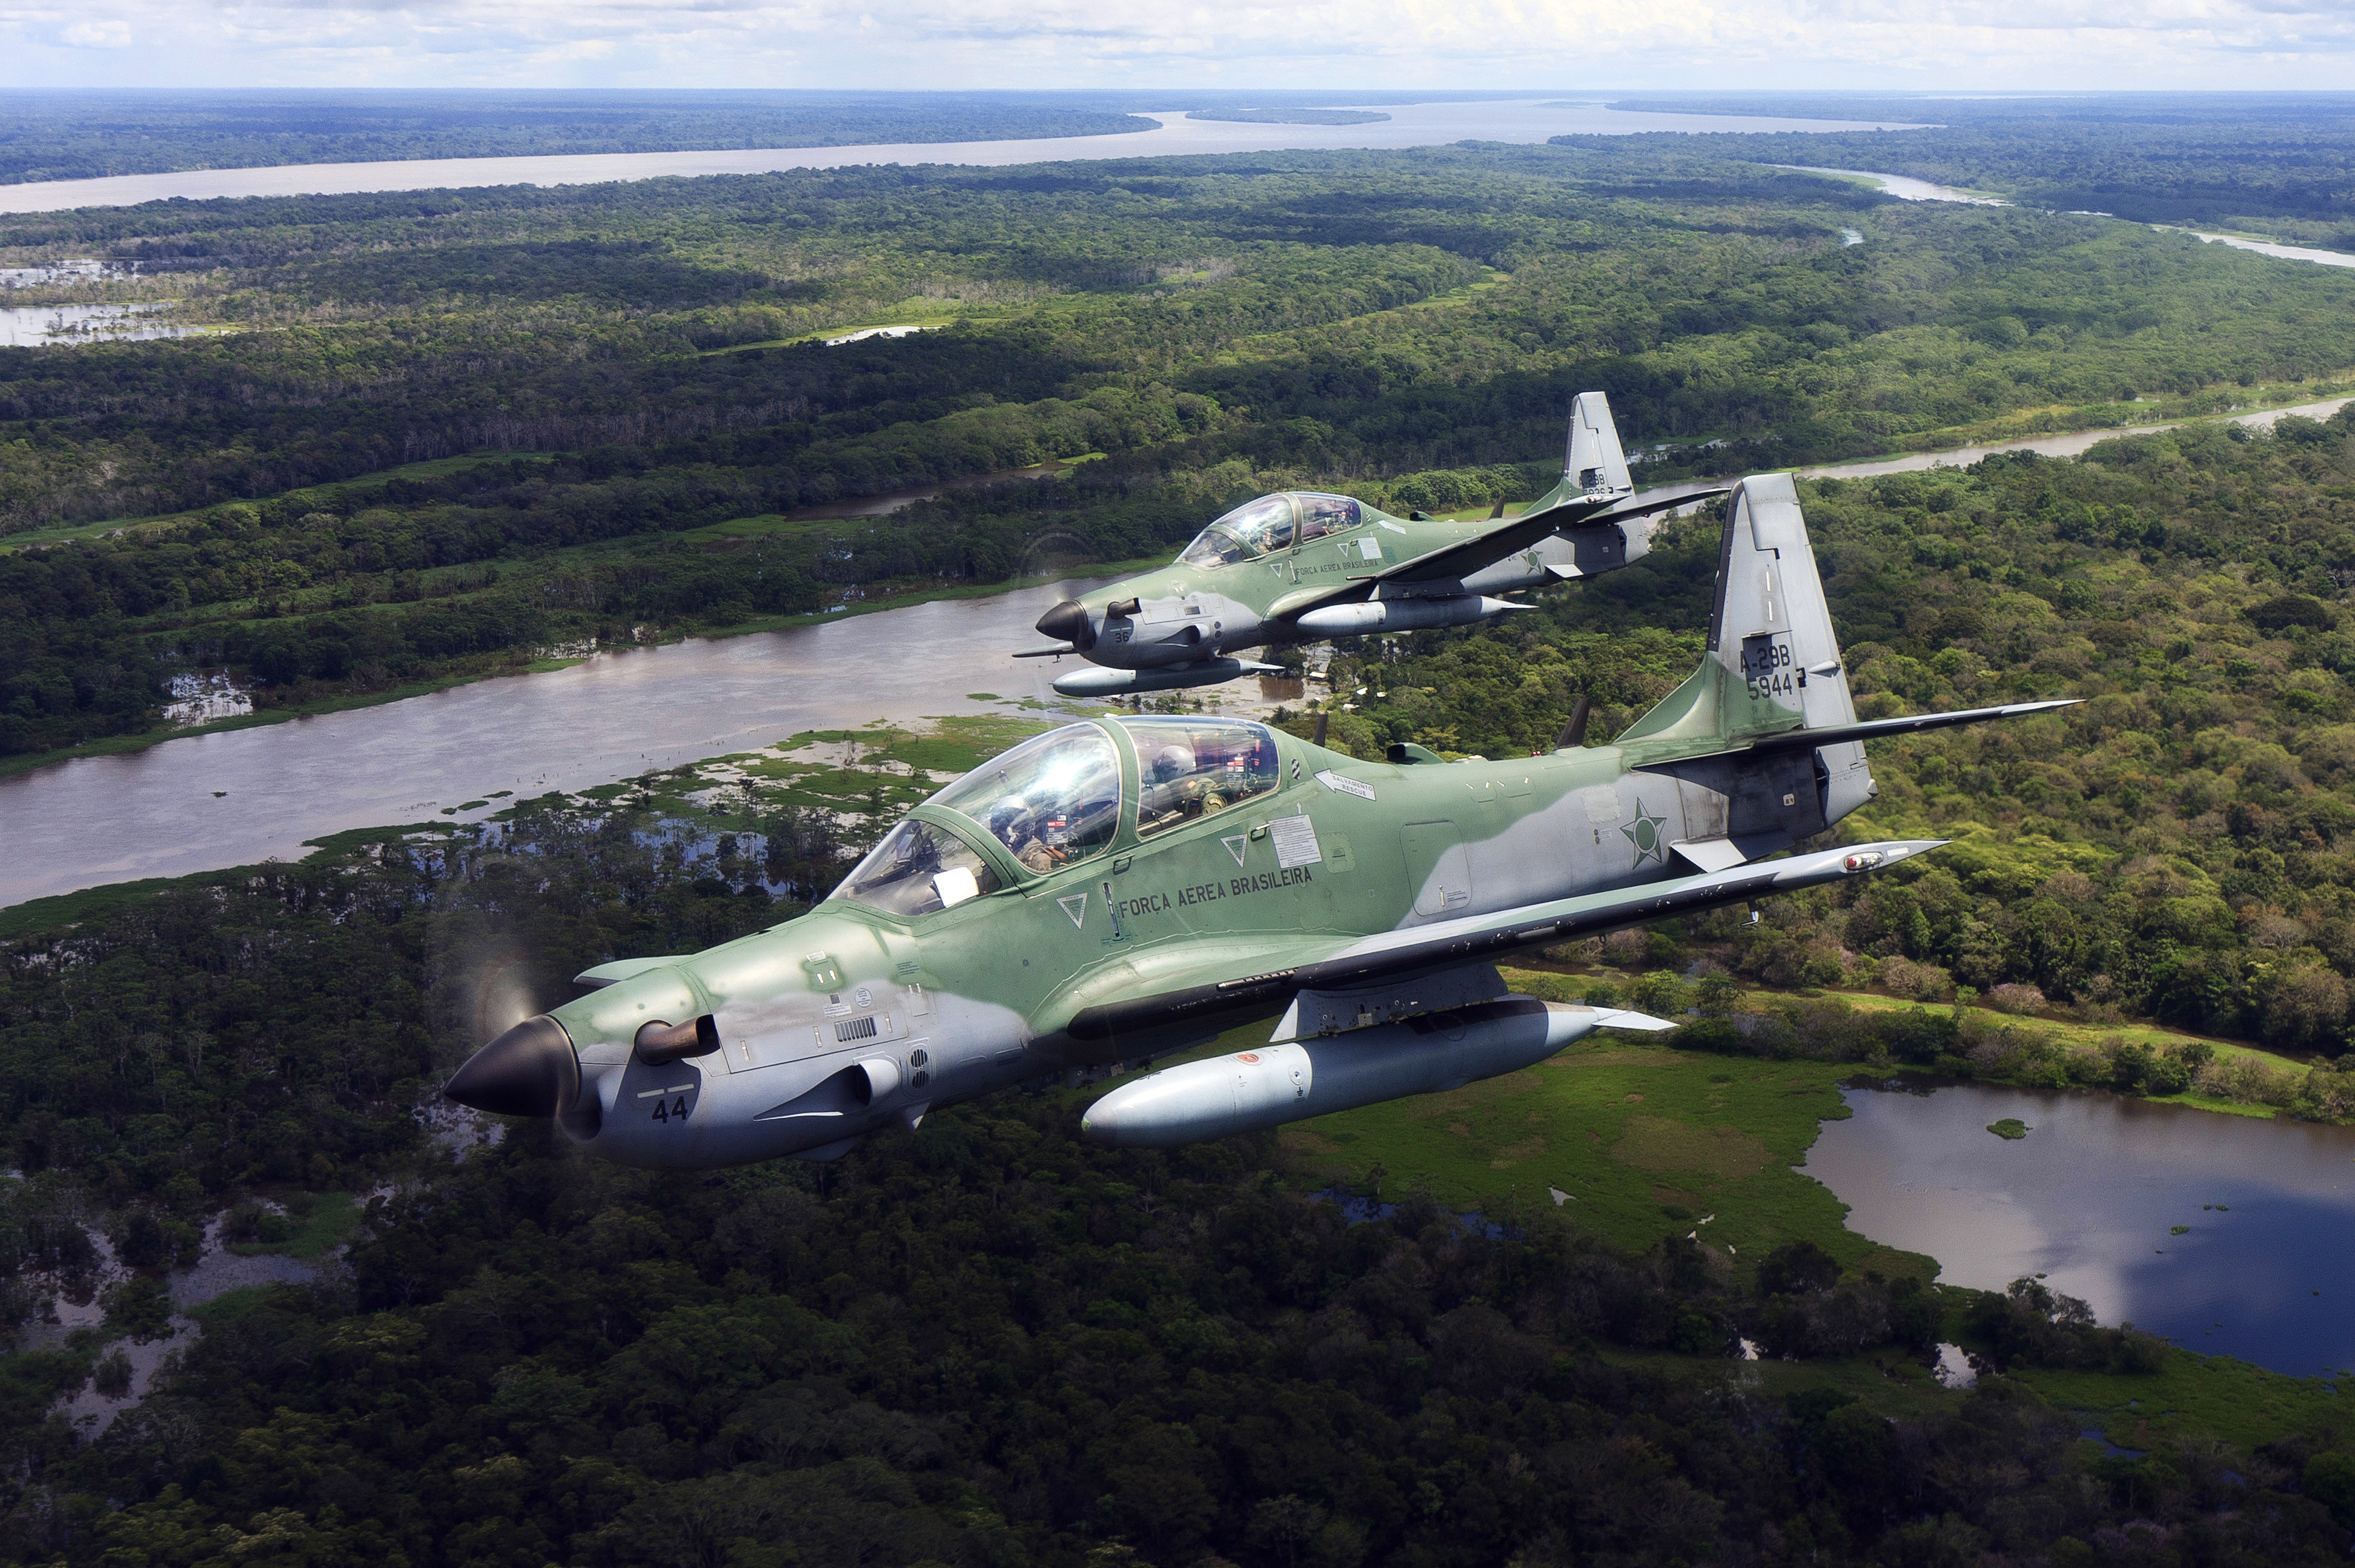
\includegraphics[trim=0 50 0 50, clip, width=0.8\linewidth] {figs/supertucano}
\end{minipage}}\\
\subfigure[][]{%
\label{fig:ejets}%
\begin{minipage}{0.9\textwidth}
\centering
\includegraphics[trim=100 0 100 0, clip, width=0.8\linewidth]{figs/embraerE}
\end{minipage}}%
\end{center}
\vspace{1.5em}
\FONTE{(a) \href{https://es.wikipedia.org/wiki/Embraer_Legacy_600}{Wikipedia: Embraer Legacy 600} (b) \href{https://es.wikipedia.org/wiki/Embraer_EMB_314_Super_Tucano}{Wikipedia: Embraer EMB 314 Super Tucano} (c) \href{http://www.embraercommercialaviation.com}{Embraer Commercial Aviation}}
\end{figure}

Another institution that works with aerospace structures is the National Institute for Space Research (in portuguese \textit{Instituto Nacional de Pesquisas Espaciais} (INPE)). INPE develops satellites for Earth observation, in projects together with other countries such as China, India, and Russia. Examples of satellites developed by INPE are the Data Collection Satellite (SCD-1 \cite{SCD1} and SCD-2, see \autoref{fig:scd}), the China-Brazil Earth Resources Satellite Program (CBERS-1, CBERS-2, CBERS-2B, CBERS-3, CBERS-4, \cite{CBERS}, see \autoref{fig:cbers}) and the Amaz\^onia project (Amaz\^onia-1, \cite{AMAZONIA}, see \autoref{fig:amazonia}).

\begin{figure}[H]%
\centering
\caption[INPE satellites]{INPE satellites:
\subref{fig:scd} SCD-1;
\subref{fig:cbers} CBERS-3;
\subref{fig:amazonia} Amaz\^onia-1}%
\label{fig:satellites}%
\subfigure[]{%
\label{fig:scd}%
\begin{minipage}{0.45\textwidth}
\centering
\includegraphics[trim=5 5 5 5, clip, width=0.4\textwidth]{figs/scd1_2}
\end{minipage}}
%
\subfigure[]{%
\label{fig:cbers}%
\begin{minipage}{0.45\textwidth}
\centering
\includegraphics[width=0.7\textwidth]{figs/CBERS4}
\end{minipage}}\\
\subfigure[]{%
\centering
\label{fig:amazonia}%
\begin{minipage}{\textwidth}
\centering
\includegraphics[width=0.7\textwidth]{figs/amazonia}
\end{minipage}}%
\vspace{1.5em}
\FONTE{(a) \href{http://www.inpe.br/scd1/site_scd/scd1/osatelite.htm}{INPE: \textit{Satélite SCD-1}} (b) \href{http://www.cbers.inpe.br/sobre_satelite/lancamento_cbers4.php}{INPE: \textit{Lançamento CBERS-4}} (c) \href{http://www.inpe.br/amazonia-1/sobre_satelite/}{INPE: \textit{Miss\~ao Amazonia-1}}}
\end{figure}

The design of an adequate computer model for the structural analysis is fundamental in the development and construction process of engineering structures.  Computer-Aided Engineering (CAE) is the extensive use of computer software to assist in engineering analysis tasks, including Finite Element Analysis (FEA), Computational Fluid Dynamics, Multibody Dynamics, and optimization of products or processes. Some examples of computer software for solving problems by the FEA are Algor, Abaqus, ANSYS, COSMOS/M, T-STRUDL, MARC, MSC/NASTRAN, NISA, Pro/MECHANICA, SAP2000, and STARDYNE \cite{logan2011first}. Those programs are widely used in the designing and analysis processes of structures in aerospace industry \cite{Birtles1983}. For example, Embraer and INPE adopted the NASTRAN, which performs different engineering analysis, such as static, dynamic, and thermal analysis.

Aerospace structures are critical systems. Failures in structures would cause catastrophic consequences, with human and material losses. Hence, it is essential to have the capability of detecting damages in an early stage, with accuracy, and safely. This detection should help to repair or rehabilitate a structure before it has major damages.

Structural health monitoring (SHM) is an important application of the field of System Identification that combines the advances of sensing technologies with theories and techniques for nondestructive damage detection (NDD). One relevant capability of SHM is its ability to monitor a structure during its operation. 

In Brazil, efforts are being made to develop a Brazilian technology in the solution of practical problems of great interest to the aerospace industry, such as Structural Damage Identification.

\section{Damages}

Damages can be defined as changes to the material or geometric properties of a structure, including changes in the boundary conditions and the system connectivity, which affect its current or future performance. The damage identification is linked to a comparison of two different states of a structure, one of which is the initial state, named undamaged, and the other is the current structural response under a forcing term. The existence of damage does not imply that the system/structure losses all its functionality, but rather that it does not operate in its standard manner.

Examples of damages are, among others, cracks, local plasticity, delamination and debonding in composite materials.

A damage can be categorized in accidental damage, fatigue damage, or environmental damage \cite{baaran2009, venterink2017frequency}. Damages associated with fatigue or corrosion in metals can accumulate incrementally over periods of time. For composites, inspection of fatigue and environmental damages are often not required, if proper design precautions were taken.

In short time-scales, accidental damages can be the result of scheduled discrete events such as aircraft landings, or unscheduled events, such as bird-strikes in aircraft or natural phenomena hazards.

As damages increase, the system/structure operation will be no longer acceptable to the user, i.e., a failure will occur. An unpredicted structural failure can cause catastrophic loss of economic value and human life.

Damages in aerospace structures can be categorized according to their severity \apud{ilcewicz2006composite}{baaran2009}:

\begin{enumerate}
    \item Allowable damage that may go undetected by scheduled or direct field inspection, for example, allowable manufacturing defects, but also non-allowable damage: Barely Visible Impact Damage (BVID), e.g., damage caused by debris or hailstones.
    \item Damage detected by scheduled or direct field inspection at specified intervals, e.g. exterior skin damage, or interior stringer blade damage.
    \item Obvious damage detected within a few flights by operations, e.g. accidental damage to the lower fuselage, or lost bonded repair patch.
    \item Discrete source damage immediately known by the pilot limiting flight maneuvers, e.g. rotor disk cut through the fuselage or severe rudder lightning damage.
    \item Severe damage created by anomalous ground or flight events, e.g. bird-strike, maintenance jacking incident, propeller mishap.
\end{enumerate}

\section{Structural damage identification}
The Structural Damage Identification (SDI) process involves the conjunction of five disciplines \cite{farrar2010introduction, Farrar2007c}:

\begin{description}[style=sameline]
\item[Structural Health Monitoring] SHM performs a global damage identification for aerospace, civil and mechanical engineering infrastructure, and it can be performed off-line as well as on-line.  On-line refers to the monitoring during operation of the system or structure, while off-line refers to the monitoring during maintenance;
\item[Condition Monitoring] Condition Monitoring is analogous to SHM, but in rotating and reciprocating machinery;
\item[Non-Destructive Evaluation] Non-Destructive Evaluation carried out off-line in a local manner after the damage has been located;
\item[Statistical Process Control] Statistical Process Control is based on process and uses a variety of sensors to monitor changes in a process;
\item[Damage Prognosis] Damage Prognosis evaluates the damage evolution and predicts the remaining useful life of a system.
\end{description}

All these processes involve the observation of a structure or a mechanical system for a period, by mean of periodically spaced measurements; the extraction of damage-sensitive features from the measurements; and the analysis of these features to determine the current state of the structural health.

The process of damage identification involves four steps:

\begin{description}[style=sameline]
\item[Operational Evaluation] Gives details of the implementation of the process, such as possible failure modes, operational and environmental conditions, and limitations related to data acquisition.
\item[Data Acquisition] Defines the quantities to be measured, the amount of data to be saved, and how the data will be acquired (which and how many sensors will be used, and where the sensors will be placed). Also, defines the data fusion and cleansing, that determine which data is necessary and useful in the feature extraction process.
\item[Feature Extraction] Identifies damage sensitive parameters from measured data.
\item[Classification] Performs the comparison between the damaged and undamaged states and quantifies the damage.
\end{description}

An ideal robust damage identification scheme should be able to detect a damage at a very early stage, locate the damage within the sensor resolution, provide an estimate of the extent or severity of the damage, and predict the remaining useful life of the structural component when the damage is identified. The identification should be independent of changes in the operational and environmental conditions. The method should also be well suited to automation and should be independent of human judgment and ability \cite{Doebling1996}.

\subsection{Classification of the Structural Damage Identification methods}
Damage identification methods can be classified in different ways: according to their performance, and to whether they are local or global, model or non-model based, and whether they use a baseline or not. 

\textbf{Performance}
The damage identification process for a system of a structure can by classified attending five levels of performance \cite{Rytter1993,Sohn2004, Worden2004, Worden2007}:

\begin{description}[style=sameline]
\item[Level 1: Detection] Verification of the presence of damage in a structure
\item[Level 2: Location] Determination of the location of the damage
\item[Level 3: Type] Determination of the type of the damage
\item[Level 4: Extension] Estimation of the extent and severity of the damage
\item[Level 5: Prognosis] Prediction of the remaining service life of the structure
\end{description}

The first four levels (Detection, Location, Type, and Extension) are related to the damage diagnosis, while the fifth step is related to the damage prognosis. Increasing the level implies a higher degree of complexity and a greater necessity of mathematical models.

\textbf{Local or global methods}

This classification is related to the inspection domain concerning the structure \cite{Fritzen2009}:

\begin{description}[style=sameline]
\item[Local] Concentrated on a specific part of the structure.
\item[Global] The whole structure is analyzed.
\end{description}

Local methods are usually considered to be more sensitive than global methods. Local methods are capable of detecting small damages, while global ones can identify only relatively severe damages. However, local methods are applicable with a prior knowledge of the location of a damaged area of the structure.

\textbf{Model or non-model based approach}

Methods can also be classified on model and non-model based:

\begin{description}[style=sameline]
\item[Non-model based] The response of the structure in service is compared with results of a reference measurement previously acquired. Deviations in damage sensitive parameters are used to identify damage.
\item[Model based] The response is compared with the results obtained from an analytical or numerical model.
\end{description}

Advantages of model based over the non-model based techniques include the possibility of the former to be easily extended to provide information about the severity of the detected damage and can be used to account for environmental or operational variations (e.g. temperature, boundary conditions, etc.). Disadvantages include the difficulty in obtaining an accurate model representation of complex structures, and its limited applicability for \textit{in situ} monitoring, due to their computational cost.

\textbf{Baseline or non-baseline}

The process of identifying a damage requires the comparison of two states, one of them being the undamaged reference. Therefore, methods can also be classified according to whether  a baseline is used or not \cite{Worden2007}:

\begin{description}[style=sameline]
\item[Baseline] The response of the structure, measured at an earlier stage, is usually utilized as a baseline to distinguish between the damaged and undamaged states.
\item[Non-baseline] The response is compared with a state of the structure assumed to have a normal behavior (e.g. a smooth pattern or linear-elastic response). The system is in this case classified as damaged when the response deviates from the expected behavior.
\end{description}

SDI can be treated as two complementary approaches \cite{Montanari2014}:
\begin{description}[style=sameline]
\item[Inverse problem] This approach typically uses a model of the structure and tries to relate changes in measured data from the structure to changes in the model \cite{friswell2007damage}. Locally linearized models are sometimes used to make the analysis simpler. The behavior of the real structure is compared to the corresponding model, through optimization algorithms.
\item[Pattern recognition problem] This approach follows the concepts of the Pattern Recognition (PR) problem \apud{schalkoff1992pattern}{Montanari2014}
\end{description}

\section{Literature overview of techniques for Structural Damage Identification}
\label{chap:state}

A high amount of Non-Destructive Evaluation (NDE) techniques can be used for damage identification. Most of them can only be applied off-line. Thus, only a minor quantity of these techniques can be used in an SHM system.

\autoref{fig:methods} shows a scheme of these techniques (first three lines), that include the Structural Vibration (SV) and Electromechanical Impedance (EMI) techniques which primarily rely on standing wave patterns. Another group, including the higher frequency Acoustic Emission (AE), Acousto-Ultrasonic (AU), and Ultrasonic Testing (UT), employ traveling wave characteristics.

SV and EMI provide results that are relatively easy to interpret. More complex structures can be analyzed with these methods, allowing to explore outright a relatively large area. However, in these methods the limited frequency range causes a limited resolution, and only relatively severe damage, such as delaminations, can be identified.

AE, AU and UT can all detect small damages, such as cracks. For this reason, these wave based technologies are more frequently used for aircraft applications \cite{Staszewski2009,Diamanti2010}. However, the interpretation of the data is more complicated than with SV and EMI, especially in the case of non-flat or composite structures \cite{Dalton2001}.

\begin{sidewaysfigure}
\caption{Overview of damage identification methods. The branch of vibration-based methods is detailed with different features and classifiers used in the literature}
\label{fig:methods}
\centering
\vspace{1em}
\resizebox{\textwidth}{!}
{
\includegraphics{images/chapter1_methods.tikz}
}
\vspace{1em}
{\footnotesize SOURCE: Adapted from \cite{Ooijevaar2014}}
\end{sidewaysfigure}

\begin{table}[H]
    \caption{Dynamics based NDE technologies}
    \label{tab:my_label}
    \centering
    \footnotesize
    \begin{tabular}{cccccc}
        \toprule
        Technology & \specialcell{Frequency\\range [Hz]} & \specialcell{Actuation\\approach} & \specialcell{Sensitivity\\to damage} & \specialcell{Ease of data\\interpretation} & \specialcell{Applicability\\for SHM} \\
        \midrule
         SV & $10^0 - 10^4$ & Active / passive & ++ & +++ & ++++ \\
         EMI & $10^3 - 10^5$ & Active & +++ & +++ & ++++ \\
         AE & $10^4 - 10^6$ & Passive & ++++ & ++ & +++ \\
         AU & $10^4 - 10^6$ & Active & ++++ & + & ++++ \\
         UT & $10^5 - 10^7$ & Active & +++++ & ++ & + \\
         \bottomrule
    \end{tabular}
    \FONTE{Adapted from \cite{Ooijevaar2014}}
\end{table}

Vibration-based SHM and damage detection techniques receive a great attention in the aeronautic engineering field \cite{Liu2012}. A good system for SHM can increase the efficiency of structural maintenance, reducing the cost and enhancing the reliability of the structures \cite{de2016shm}.

\subsection{Methods based on structural vibration for structural damage identification}
\label{sec:methods}

The literature dealing with SV methods is vast. Different methods are classified depending on their approach, e.g., frequency changes, mode shape changes, dynamically measured flexibility, matrix update methods, nonlinear methods, Neural Networks-based methods, and other methods. These kind of methods are the subject of books \cite{Balageas2006,Boller2009}, doctoral theses \cite{Ooijevaar2014,de2016shm}, and review papers, some of them on specific topics (composite materials, strain based methods, nonlinear methods) \cite{Doebling1996,Doebling1998,Zou2000,Sohn2004,Carden2004,Montalvao2006,Fassois2007,Worden2008,Jhang2009,Fritzen2009,Li2010,Fan2011}. \autoref{fig:methods} summarizes the principal damage sensitive features and classifiers found in the literature on the Vibration-based Damage Identification methods category. These methods can be divided into three principal areas: time, frequency and modal domains. \autoref{tab:features} shows an overview of these features, while \autoref{tab:alldomains} in \autoref{app:A} shows a more detailed list of classifiers associated with the features.

\citeonline{Doebling1998} affirmed that sufficient evidence exists to promote the use of measured vibration data for damage identification in structures, using forced-response tests and long-term monitoring of ambient signals.

\begin{table}[H]
    \caption{Overview of the vibration based damage features}
    \label{tab:features}
    \centering
    \scriptsize
    \begin{tabular}{L{0.2\textwidth}L{0.2\textwidth}L{0.2\textwidth}L{0.2\textwidth}}
        \toprule
         Time & Time-frequency & Frequency & Modal \\
         \midrule
         Time response / waveform & Wavelet transform & Fourier / power spectra & Natural frequencies \\
         Statistical time series analysis & Hilbert transform & Frequency response function & Mode shape \\
         & Hilbert-Huang transform & Frequency response function curvature & Mode shape curvatures \\
         & & Mechanical impedance & Modal damping \\
         & & Transmissibility function & Dynamic stiffness \\
         & & Anti-resonances & Dynamic flexibility \\
         & & Higher harmonics (nonlinear) & Updating methods \\
         & & Modulation (nonlinear)\\
         \bottomrule
    \end{tabular}
    \FONTE{Adapted from \cite{Ooijevaar2014}}
\end{table}

\subsection{Metaheuristics applied to structural damage identification}

\autoref{tab:intelligence} shows a compilation of papers where the SDI problem is approached using different Computational Intelligence techniques. They can be divided into five groups: neural network techniques, support vector machine, fuzzy inference, metaheuristic algorithms, and hybrid techniques. Among them, the formulation of the SDI problem as a constrained optimization problem is typically considered the most effective strategy \cite{Yu2011}.

Some authors have used the classic Genetic Algorithm (GA) for solving the Damage Identification problem. For instance, \citeonline{Mares1996} located and quantified damages in truss and beam structures; \citeonline{Borges2007} identified damages in a framed structure; and recently, \citeonline{Boonlong2014} used Cooperative Coevolutionary Genetic Algorithm as the optimizer for the vibration-based damage detection in beams.

Other classical metaheuristics have also been used for this purpose. A continuous variant of Ant Colony Optimization (ACO) was used by \citeonline{Yu2011} to detect single and multiple damages on 2 and 3-storey building models; they suggested the use of hybrid approaches of ACO to improve the results. In \citeonline{Braun2015}, different versions of ACO, as well as hybrid variants using HJ, were used to detect damages on a damped spring-mass system.

A combination of a self-configurable Particle Swarm Optimization (PSO) with the Nelder-Mead (NM) algorithm has also been used for optimal localization of sensors for health monitoring \cite{rao2007optimal}. In \citeonline{abdalla2009particle}, PSO was also applied in the solution of the inverse problem of structural damage identification using a cantilever beam model. The hybrid PSO-simplex (PSOS) was used in two structural damage identification problems with noisy and incomplete data, in the frequency domain. \citeonline{begambre2009hybrid} used Latin hypercube sampling and PSO for an experimental verification of the structural damage detection process. \citeonline{kang2012damage} proposed an immunity enhanced particle swarm optimization (IEPSO) algorithm for damage detection, which was used for a simply supported beam, and on a plane truss structure. Also, \citeonline{VakilBaghmisheh20122217} hybridized PSO with NM for crack detection in cantilever beams.

Recently, the novel Bird Mating Optimizer (BMO) was used in \citeonline{Zhu2017} for identifying structural damages using the minimization of the differences between the measured and calculated natural frequencies and correlation function acceleration vector of damaged and undamaged structures. This method was used for identifying damages on a planar frame structure, and a three connected shear building.

This topic has served to present new metaheuristics. For example, the Big Bang-Big Crunch (BBC), in \citeonline{Tabrizian2013}, is used to identify damages in beam bridges, a Belgian truss, and a two-story two-bay frame. In their work, this algorithm minimizes an objective function using complete and incomplete modal data, with and without noise. In \citeonline{Yu2014}, single and multiple damage cases are detected in a simulated 4-storey benchmark frame structure, and in a 2-storey rigid frame, using the global Artificial Fish Swarm Algorithm (GAFSA). Also, an experimental laboratory study on damage detection was performed in a 3-storey building model, with four damage patterns. \citeonline{Ding20161} presented the quick ABC (QABC), an artificial bee colony (ABC) algorithm with hybrid search strategy based on modal data. QABC is applied in the damage identification of a truss and a plate.

{
\scriptsize
\centering
\renewcommand{\arraystretch}{0.9}
\begin{longtable}{L{8.2cm}L{5.8cm}}
\caption{Literature overview of Computational Intelligence methods used for SDI}
\label{tab:intelligence}
\endfirsthead
\multicolumn{2}{c}%
{\tablename\ \thetable\ -- \textit{Continued from previous page}} \\
\toprule
\endhead
\midrule \multicolumn{2}{r}{\textit{Continued on next page}} \\
\endfoot
\midrule
\endlastfoot
\toprule
\multicolumn{2}{l}{\textbf{Neural networks}}\\
\midrule
Iterative Neural Network (INN) & \cite{Chang2000}\\
Backpropagation NN (BP-NN) & \cite{Zang2001}\newline \cite{Yam2003a}\newline \cite{Pawar2006}\newline \cite{Mehrjoo2008} \newline \cite{Chiwiacowsky2008}\\
Multilayer Neural Network (MNN) & \cite{Huang2001}\\
Extended Kalman Filter Trained Neural Network (EKFNN) & \cite{Jin2016}\\
\midrule
\multicolumn{2}{l}{\textbf{Support Vector Machine (SVM)}}\\
\midrule
Hyper-Solution SVM (HSVM) & \cite{Candelieri2014}\\
\midrule
\multicolumn{2}{l}{\textbf{Fuzzy}}\\
\midrule
Fuzzy Clustering (FC) & \cite{Silva2008}\\
Fuzzy Logic System (FLS) & \cite{Chandrashekhar2009}\\
\midrule
\multicolumn{2}{l}{\textbf{Metaheuristics}}\\
\midrule
Genetic Algorithm (GA) & \cite{Boonlong2014} \newline \cite{Borges2007} \newline \cite{Chou2001} \newline \cite{Gomes2008} \newline \cite{Mares1996}\\
Improved PSO (IPSO) & \cite{Yu2008}\\
Tabu Search (TS) & \cite{Arafa2010}\\
Continuous ACO (CnACO) & \cite{Yu2011}\\
Ant Colony Optimization (ACO) & \cite{Majumdar2012} \newline \cite{Yu2011}\\
Swarm Intelligence (SI) & \cite{Yu2012} \\
Particle Swarm Optimization (PSO) & \cite{Mohan2013} \newline \cite{Seyedpoor2012}\\
Big Bang-Big Crunch (BB-BC) & \cite{Tabrizian2013}\\
Simulated Annealing (SA) & \cite{Kourehli2013}\\
Differential Evolution (DE) & \cite{Fu2014} \newline \cite{Seyedpoor2015} \newline \cite{Seyedpoor2015a}\\
Charged System Search (CSS) & \cite{kaveh2015improved}\\
 Multi-Swarm Fruit Fly Optimization Algorithm (MFOA) & \cite{li2015multi} \\
Global Artificial Fish Swarm Algorithm (GAFSA) & \cite{Yu2014} \\
Rank-based Ant System (RAS) & \cite{Braun2015}\\
Ant System with Heuristic Information (ASH) & \cite{Braun2015}\\
Elitist Ant System (EAS) & \cite{Braun2015}\\
Firefly Algorithm (FA) & \cite{Pan2015} \\
Cyclical parthenogenesis algorithm (CPA) &
\cite{Kaveh2017} \\
\midrule
\multicolumn{2}{l}{\textbf{Hybrid algorithms}}\\
\midrule
Genetic Algorithm + Conjugated Gradient Method (GA-CGM) & \cite{Chiwiacowsky2006} \newline \cite{Chiwiacowsky2006b}\\
Genetic Algorithm + Levenberg-Maquardt (GA-LM) &\cite{He2006} \\
Genetic Fuzzy System (GFS) & \cite{Pawar2007}\\
Simulated Annealing Genetic Algorithm (SAGA) & \cite{Kokot2009} \\
Genetic Algorithm and Particle Swarm Optimization (GA-PSO) & \cite{Sandesh2010}\\
Ant System with Heuristic Information + Hooke-Jeeves (ASH-HJ) & \cite{Braun2015}\\
PSO with Nelder-Mead (PSO-NM) & \cite{Chen2015}\\
Multi-Particle Collision Algorithm with Hooke-Jeeves (MPCA-HJ) & \cite{HernandezTorres2015b}\\
$q$-Gradient with Hooke-Jeeves ($q$G-HJ) & \cite{HernandezTorres2015} \\
Firefly Algorithm / Genetic Algorithm & \cite{khatir2016multiple}\\
Quick Artificial Bee Colony algorithm (QABC) & \cite{Ding20161}\\
Particle Swarm Inspired
Multi-Elitist Artificial Bee Colony (PS-MEABC) & 
\cite{Fatahi2017}\\
\bottomrule
\end{longtable}
}

\subsection{Gaps found in the literature}

As discussed in \autoref{sec:methods}, many damage identification techniques have been proposed in the literature. However, their practical application can be difficult \cite{Doebling1998,Ooijevaar2014}.

There are uncertainties in damage identification \cite{xu2017smart}, mainly caused by:
%Smart Civil Structures
\begin{itemize}
    \item Methodology errors:
    \vspace{0.5em}
    \begin{itemize}
    \item Limitations of the damage identification methods;
    \end{itemize}
    \vspace{-0.5em}
    \item Modeling errors:
    \vspace{0.5em}
    \begin{itemize}
    \item Inaccuracy in the discretization of the FE model;    
    \item Uncertainties in the geometry and boundary conditions;
    \item Variations in material properties;
    \item Operational and environmental variability;
    \end{itemize}
    \vspace{-0.5em}
    \item Measurement errors:
    \vspace{0.5em}
    \begin{itemize}
    \item Errors in the measured signals, caused by noise, or by procedures in the measurements;    
    \item Errors in the post-processing techniques;
    \end{itemize}
\end{itemize}

Some issues that need to be solved to enable the actual practice of these methods are summarized below:

\begin{description}[style=sameline]
\item[Lack of robustness] None of the methods solves all problems for all structures.

\item[Occurrence of False alarms] One of the main challenges in damage identification is the development of methods that provide a high detection probability, without false alarms. There are two types of false damage identification: \textit{false-positive}, when a intact element is identified as damaged, and a \textit{false-negative}, that is a failure in identifying damaged elements. A false-negative can cause serious life and safety consequences, while a false-positive causes a decrease in the reliability of the method.

\item[Low-performance level] Most of the methods attends the first two levels of performance (detecting and locating damage), but they are limited in their capability to achieve a prognosis, as well as in classifying the type and severity of the damage \cite{Ooijevaar2014}. The prognosis is the prediction of the remaining lifetime of the structure through the analysis of the damage evolution. It represents an important step for the development of autonomous systems for monitoring the structural health.

\item[Low complexity structures] Most of the methods deals with relatively low complexity structures (simple concrete or metallic structures, or relatively simple composite beams and plates structures). These structures are typically well-defined, or the damage scenario is created artificially. It is necessary to focus on more specific applications, such as real life and industrial structures like air-frames, bridges, and other long design life structures with life-safety or economic implications.

\item[No integration with engineering software] CAE software help in the task of modeling and analyzing structures. Among the papers revised, the use of these computer programs is scarcely mentioned.

\item[No operational and environmental variability] In real applications, the operational and environmental conditions, such as temperature and wind, could mask or modify the effects of the damages. Good approaches should have the capability of to separate their effects.

\item[Integrated sensor and network] Another problem is related to the optimal quantity and location of the sensors because they are expensive. Also, obtaining many signals increases the computational cost, and could add errors due to the inherent noise of the sensors and some possible external noises.

\item[Cooperation] Due to the magnitude of the projects, more cooperation is required between academia and industry.
 
\end{description}

More detailed discussions on these problems are provided by \citeonline{farrar2007introduction} and \citeonline{boller2013structural}.

In this thesis, the SDI will be defined as an inverse problem and solved as an optimization problem.

\section{Research objective}

The main objective of this thesis is:

\begin{quote}
To develop hybrid metaheuristics for identifying damages on structures modeled in FORTRAN and NASTRAN, using a hierarchical approach.
\end{quote}

This work will contribute to the improvement of the Multi-Particle Collision Algorithm and the $q$-gradient method, to the creation of hybrid algorithms, and to their application in the development of a tool to assist the implementation of structural health monitoring technology in aerospace structures.

\subsection{Tasks}

Specific tasks and sub-tasks were also defined to accomplish the main objective:

\begin{enumerate}
\item Perform a literature review on methods for Damage Identification;
\item Perform modifications in the Multi-Particle Collision Algorithm, for performance improvement;
\vspace{0.5em}
\begin{enumerate}
\item Modificate functions for improving the exploration and the exploitation of the algorithm;
\end{enumerate}
\item Develop hybrid algorithms based on MPCA and $q$-gradient, using concepts derived from the Opposition Based Learning, and the direct-search method Hooke-Jeeves;
\item Identify damages on structures with different complexities implemented in FORTRAN;
\vspace{0.5em}
\begin{enumerate}
\item Model structures with different types and complexities in FORTRAN;
\item Identify damages on structures implemented using finite elements on FORTRAN using hybrid algorithms;
\end{enumerate}
\item Identify damages on structures with different complexities modeled on NASTRAN;
\vspace{0.5em}
\begin{enumerate}
\item Model structures with different types and complexities in NASTRAN;
\item Identify damages on structures modeled on NASTRAN using hybrid algorithms;
\end{enumerate}
\item Identify damages on structures modeled on NASTRAN using a hierarchical approach;
\vspace{0.5em}
\begin{enumerate}
\item Identify damages on structures with medium complexity, through the hierarchical approach, using hybrid algorithms.
\end{enumerate}
\end{enumerate}

\section{Outline}

This thesis is structured into ten chapters, including introduction and conclusions, and three appendixes, organized as follow:

\begin{description}[style=sameline,labelindent=1cm]
\item [\fullref{chp:1} (this chapter)] In this chapter, the research objective and main tasks are defined.
\item [\fullref{chp:3}] 
\item [\fullref{chp:4}] In this chapter, the transient response analysis of structures is presented as the forward model. The mathematical definition and the numerical solution of direct and modal methods is summarized. Then, the Finite Element Method is introduced and presented the explanation of how it is applied in computing the model of systems with springs, and structures with bars and beams.
\item [\fullref{chp:5}]
\item [\fullref{chp:6}]
\item [\fullref{chp:7}]
\item [\fullref{chp:8}]
% \item [\fullref{chp:9}]
\item [\fullref{chp:10}]
\item [References]
\item [\fullref{app:A}] This appendix presents the main features and classification approaches found in the literature, with an exhaustive bibliographic revision.
\item [\fullref{vita}] This annex presents the vita of the author of this thesis, including full papers on journals, national and international congresses, that directly or indirectly contributed to the doctoral thesis.

\end{description}

%\include{docs/chapter2}
\chapter{Vibration-based Damage Identification solved as optimization problem}
\label{chp:3}
\epigraph{A problem well-stated is a problem half-solved.}{John Dewey}

\tikzstyle{spring}=[thick,decorate,decoration={zigzag,pre length=0.5cm,post length=0.5cm,segment length=15,amplitude=1em}]

In the first chapter, the main concepts on the SDI were introduced. A literature review was done on the different methods for SDI, and the classification of those methods was presented.

In this chapter, the Vibration-based Damage Identification (VDI) will be defined as an optimization problem.

First, the main concepts about inverse problems in engineering will be presented. Then, the VDI will be defined as an optimization problem, and the damage parameters and the objective function will be defined.

\section{Basic concepts of optimization}

Optimization is the area of the Applied Mathematics that studies the theory and techniques to find the best available values to optimize (minimize or maximize) some objective function, also called error function or cost function. Typical applications of optimization are to find the minimal cost, maximal profit, minimal error, optimal design and optimal management. Many books handle the concepts of the optimization area, such as \citeonline{rothlauf2011design}.

\begin{definition} 
An \textbf{optimization problem} is the problem of finding the best solution from all feasible solutions. 
\end{definition}

A solution is \textbf{feasible} if it satisfies all constraints.

\begin{definition}
A \textbf{candidate solution} $s$ is an element of the search space $\mathcal{S}$ of a certain optimization problem.
\end{definition}

\begin{definition}
The \textbf{search space} $\mathcal{S}$ of an optimization problem is the set containing all element $s$ which could be its solution.
\end{definition}

An optimization problem can be classified depending on the existence of constraints. In an \textbf{unconstrained} optimization problem, the objective function depends on variables with no restrictions, and in a \textbf{constrained} optimization problem, the objective function is subject to constraints on the variables.

\begin{definition}
The standard form of a unconstrained optimization problem is:
%
\begin{align}
\begin{split}
    \underset{s}{\text{minimize}} \quad & J_i(s) \; i = 1, \cdots, n_j \\
    \text{subject to} \quad & s \in \mathcal{S}
\end{split}
\end{align}
%
where $s = \left( s_1, s_2, \cdots s_D \right)$ is a vector of $D$ \textbf{decision variables}, and $J_i: \R^D \to \R$ are the \textbf{objective functions} (also known as error functions, or cost functions depending on the problem to be solved) to be minimized over the variable $s$, and $\mathcal{S} = \R^D$.

\end{definition}

\begin{definition}
The \textbf{globally optimal solution} $s^* \in \mathcal{S}$ of a objective function $J$ is defined as:
%
\begin{equation}
    J(s^*) \leq J(s) \quad \forall s \in \mathcal{S}
\end{equation}
%

\end{definition}

\begin{definition}
A \textbf{locally optimal solution} $s^\prime \in \mathcal{S}$ of a objective function $J$ with respect to a neighborhood function $\mathcal{N}$ is defined as: 
%
\begin{equation}
    J(s^\prime) \leq J(s) \quad \forall s \in \mathcal{N}(s^\prime)
\end{equation}

If $\mathcal{S} \subseteq \R^D$:

\begin{equation}
    \forall s^\prime  \exists \varepsilon > 0 : J(s^\prime) \leq J(s) \forall s \in \mathcal{S}, \mid s - s^\prime \mid < \varepsilon
\end{equation}

\end{definition}

\autoref{fig:minima} shows a graphical representation of local and global minima.

\begin{figure}[H]
\caption{Local and global minima}
\label{fig:minima}
\centering
\begin{tikzpicture}
\begin{axis}[
ymin=26,
ymax=52,
xmax=64,
xmin=0,
xticklabel=\empty,
yticklabel=\empty,
axis lines = left,
xlabel=$s$,
ylabel=$J(s)$,
label style = {at={(ticklabel cs:1)}},
y label style = {rotate=-90}
]
\addplot[smooth] coordinates {
(0,45)
(10,35)
(20,40)
(30,30)
(40,47)
(50,40)
(60,50)
};
\fill[blue] (10,35) circle (2pt) node[below] {$s^\prime$};
\fill[red] (30,30) circle (2pt) node[below] {$s^*$};
\fill[blue] (50,40) circle (2pt) node[below] {$s^\prime$};
\end{axis}
\end{tikzpicture}
\end{figure}

There are many ways for classifying the optimization problems. They can be divided into \textbf{continuous} when the variables are allowed to get any value within a range; or \textbf{discrete}, when the variables are required to belong to a discrete set. This set could be a subset of integers (called \textit{integer programming}) or a set of objects or combinatorial structures (called \textit{combinatorial optimization}). Also, exist some problems where the domain is \textbf{mixed}.

The nature of the variables divides the optimization problems into two groups: \textbf{deterministic} when the data for the given problem are known accurately, and \textbf{stochastic} or non-deterministic when some or all the design variables are probabilistic.

The optimization problems can also be classified according to the number of objective functions. A \textbf{mono-objective} problem is when there is only an objective function, while a \textbf{multi-objective} problem have more than one objective function that can be minimized or maximized simultaneously.

The standard form of a constrained mono-objective optimization problem is:
%
\begin{align}
\begin{split}
    \underset{s}{\text{minimize}} \quad &J(s) \\
    \text{subject to} \quad &g_j(s) \leq 0, \; j = 1, \cdots, n_g \\
    & h_k(s) = 0, \; k = 1, \cdots, n_h
\end{split}
\end{align}
%
where $g_j$ are called inequality constraints, and $h_k$ are called equality constraints.

\section{Inverse problems in engineering}

A model can be simply described as the relationship between the parameters and the data, that is useful for simulating and predicting aspects of the behavior of a system. A model represents a real system as symbols and using the language of other sciences. For instance, an engineering process may be modeled using mathematical symbols and computer sciences \cite{alavala2008finite}.

The process of finding data based on a model using a set of parameters as input is called as \textbf{forward problem} while estimating a set of parameters of a model based on a set of data is known as \textbf{inverse problem} \cite{CamposVelho2001problemas,silvaneto2005problemas,camposvelho2008}. A schematic representation of these processes is shown in \autoref{fig:problems}.

\begin{figure}[H]
    \caption{Schematic representation of the forward and inverse problems}
    \label{fig:problems}
    \centering
    \includegraphics{images/chapter1_forwardinverse.tikz}
\end{figure}

In an inverse problem, the \textbf{parameters} are the numerical values to be estimated, and the \textbf{data} are the observations or measurements made on the system of interest.

Inverse problems are found in almost every field of science and mathematics, such as optics, radar, acoustics, communication theory, signal processing, medical imaging, computer vision, geophysics, oceanography, astronomy, remote sensing, natural language processing, machine learning, nondestructive testing, among others.

The following three conditions were suggested by Jacques Hadamard for a well-posed problem:

\begin{enumerate}
    \item Existence: A solution of the problem exists;
    \item Uniqueness: The solution is unique;
    \item Stability: The solution depends continuously on the data.
\end{enumerate}

Usually, inverse problems violate all the three conditions, being therefore ill-posed. For handling this issue, some special methods are used, called regularization methods (e.g., Lavrentiev Regularization, Tikhonov Regularization, and Asymptotic Regularization). These methods transform an ill-posed problem into a well-posed problem, closer to the original problem. With the using of soft or regular solutions, these techniques can control the influence of the noise, and prevent over-fitting.

Some other methods for solving inverse problems are Variational method, Least squares method, filtering methods, neural networks, and Monte Carlo methods.
    
\section{Vibration-based Damage Identification as an Inverse Problem}

Dynamic processes modeling in mechanical vibration is characterized by knowing initial and boundary conditions, the geometry of the structure, material properties, and forcing terms. The system output response is the measurement of displacement, accelerations, strains, stresses, natural frequencies, and modes shapes. In vibration systems, modal parameters are a function of the physical properties of the structure (such as mass, damping, and stiffness). Therefore, a change in the physical properties (caused by cracks, loosening of connections or another possible damage) will cause detectable variations in the modal properties.

The inverse problem of damage evaluation consists in detecting, localizing and quantifying the damage severity. In this thesis, the damage severity is obtained by estimating the stiffness values from structural displacements and modal properties measurements.

The inverse problem can be formulated as an optimization problem.  \autoref{fig:opt} shows a graphical representation of the inverse solution for a generic structure. Parameter $\Theta^e$ represents the influence of environmental and operational conditions (e.g. temperature, and humidity), and $\Theta^d$ are the damage parameters (e.g. crack length, loss of stiffness, and loss of mass) \cite{Fritzen2009}. The displacements ${u}^{{mod}}$ are obtained running the structural model with a stiffness vector $k^d$, and the measured displacements ${u}^{{obs}}$ are acquired from the sensors in the vibration experiments.

\begin{figure}[H]
    \caption{Vibration-Based Damage Identification as optimization problem}
    \label{fig:opt}
    \centering
    \vspace{1em}
    \resizebox{0.8\textwidth}{!}{\includegraphics{images/chapter3_inversesolution.tikz}}
\end{figure}

\subsection{Damage parameters}
The damage parameters $\Theta^d$ are defined as the percentage of loss of stiffness at each element to be monitored:
%
\begin{equation}
\label{eq:thetad}
\Theta^d = \left( 1 - \frac{k^d}{k^i} \right) \times 100\%\,,
\end{equation}
%
where $k^d = \left(k^d_1, k^d_2, \cdots, k^d_n\right)$ and $k^i = \left(k^i_1, k^i_2, \cdots, k^i_n\right)$ are the estimated stiffness vector for the damaged system, and the stiffness vector of the undamaged system, respectively.

\subsection{Objective function}

The optimization problem can be stated as follows:
%
\begin{align}
\begin{split}
    \underset{\Theta^d}{\text{minimize}} \quad & J\left(\Theta^d\right) = \sum_{m=1}^{n_m} e_m^2\left(\Theta^d\right) \\
    \text{subject to} \quad & \Theta^{\rm d^{l}} \leq \Theta^d \leq \Theta^{\rm d^{u}}
\end{split}
\end{align}
%
where $n_m$ is the number of measured displacements, and $\Theta^{\rm d^{l}}$ and $\Theta^{\rm d^{u}}$ are the lower and upper bounds for the damage parameters, respectively.

The residuals $e_m$ are computed as:

\begin{equation}
    e_m = \sum_{t=0}^{t_f} {u}_m^{{obs}}(t) - {u}_m^{{mod}}(\Theta^d, t)
\end{equation}

in which $t$ represents the time, and $t_f$ is the final time.

\section{Hierarchical Approach}

The hierarchical search applied to the SDI follows the idea of the Latin concept \textit{Divite et impera}

Following the ``Divide et impera'' lemma appears the hierarchical approach to solve the structural damage identification problem. The idea is to reduce the computational cost in the process. The hierarchical approach for damage detection consists in three steps \cite{Santos2014}:

\begin{description}[style=sameline]
\item[First step] Define the whole structure to be analyzed, with its physical and geometric properties (length, Young module, and material density)
\item[Second step] Perform the vibration test obtaining the displacement measures in all possible points
\item[Third step] The structure is modeled in finite elements, coarsely with a low number of degrees of freedom (DOF), and the optimization problem is solved. As well as damaged areas are being detected, an iterative process of refining is performed, remodeling the area where the damage is found.
\end{description}

The third step will execute the hierarchical search, looking for damages in a sequence of refinement steps of the model. For each iteration, involving the second and the third steps, the structure will be refined, resulting with more DOF than the previous model.

\autoref{fig:hierarchical} presents a didactic example (not at all real) of damage identification on a aircraft, through the hierarchical search. The whole structure of the aircraft is represented as $\Omega$ in the \autoref{fig:aircraft1}.

\begin{figure}[H]%
\centering
\caption[Hierarchical search]{Hierarchical search:
\subref{fig:aircraft1} the whole structure;
\subref{fig:aircraft1} first stage: the aircraft is divided into six main parts;
\subref{fig:aircraft1} second stage: the tail of the aircraft is divided into more three parts \subref{fig:aircraft1} third stage: the left wing of the tail is divided into more six parts}%
\label{fig:hierarchical}%
\subfigure[]{%
\label{fig:aircraft1}%
\begin{minipage}{0.49\textwidth}
\centering
\includegraphics{images/chapter3_aircraft1.tikz}
\end{minipage}}
%
\subfigure[]{%
\label{fig:aircraft2}%
\begin{minipage}{0.49\textwidth}
\centering
\includegraphics{images/chapter3_aircraft2.tikz}
\end{minipage}}\\
\subfigure[]{%
\centering
\label{fig:aircraft3}%
\begin{minipage}{0.49\textwidth}
\centering
\includegraphics{images/chapter3_aircraft3.tikz}
\end{minipage}}
%
\subfigure[]{%
\label{fig:aircraft4}%
\begin{minipage}{0.49\textwidth}
\centering
\includegraphics{images/chapter3_aircraft4.tikz}
\end{minipage}}
\end{figure}

The first step for performing the identification process is to divide the aircraft into its six main parts, as shown in \autoref{fig:aircraft2}. Those parts are: $\Omega_{_1}$ front part of the plane body; $\Omega_{_2}$ medium part of the plane body; $\Omega_{_3}$ right wing; $\Omega_{_4}$ left wings; $\Omega_{_5}$ rear part of the plane body, and $\Omega_{_6}$ vertical and horizontal stabilizer, rudder and elevator, as a whole.

Suppose that, from the vibration test with these six elements, damage was found in $\Omega_{_6}$. The damage is identified in the \autoref{fig:aircraft2} with a small red circle. The next step is to refine this part in simpler parts. In this case, $\Omega_{_6}$ is divided in three parts , as shown in \autoref{fig:aircraft3}: right horizontal stabilizer and elevator ($\Omega_{_{6,1}}$), vertical stabilizer and rudder ($\Omega_{_{6,2}}$), and left horizontal stabilizer and elevator ($\Omega_{_{6,3}}$). Now, the forward model is run with eight gross elements.

Suppose again that in the last identification process, the damage was located in the left horizontal stabilizer ($\Omega_{_{6,3}}$). This damaged element is split into six more parts, now identified as $\Omega_{_{6,3,1}}$, $\Omega_{_{6,3,2}}$, $\Omega_{_{6,3,3}}$, $\Omega_{_{6,3,4}}$, $\Omega_{_{6,3,5}}$, and $\Omega_{_{6,3,6}}$ in the \autoref{fig:aircraft4}. Now, the identification problem is run with 13 elements. The damage should be now identified in the element $\Omega_{_{6,3,3}}$.

In this iterative process, the structure will be refined until the accuracy of the design model is reached.

\section{Chapter Conclusions}

In this chapter, the VDI was presented as an IP, more specifically as an optimization problem. The damage parameters will be used as the solution vector of the problem. The objective function to be minimized was defined as the square error between the measured data and the data obtained running the computational model of the structure. Some common models will be further discussed in the next chapter.
\chapter{Transient response analysis of structures as direct model}
\label{chp:4}
\epigraph{All models are wrong, but some are useful.}{George E. P. Box}

In the previous chapter, it was presented that the VDI will be solved as an optimization problem that uses data obtained through structural models.

In this chapter, is presented the direct model used to obtain the transient response analysis of structures. First, the transient response of a structure will be defined, and classified into the direct and the modal categories. The mathematical definition, and the numerical solution of both methods will be summarized. Then, the Finite Element Method will be introduced, and how it is applied in computing the model of systems with springs, and structures with bars and beams.

\section{Transient response analysis}

In the transient analysis, a response to a time-varying input is computed. The excitation is defined in the time domain, and the responses, such as nodal displacements and accelerations, are a function of time.

There are two categories of transient response analysis:

\begin{description}[style=sameline]
    \item [Direct transient response] carries out a numerical integration on the complete equation of motion, and
    \item[Modal transient response] uses some mode shapes, reducing the problem size. Uncouple the equations when no damping or only modal damping is used on the model.
\end{description}

Both methods will be detailed in the next sections.

\subsection{Direct transient response}
\label{sec:str}

The dynamic response of motion under kinematic excitation is shown in \autoref{eq:dynamic}:

\begin{equation}
\label{eq:dynamic}
{M}\ddot{u}(t) + {C}\dot{u}(t) + {K} {u}(t) = {F}(t)\,.
\end{equation}

In the equation, $M$, $C$ and $K$ represent the mass, viscous damping and stiffness matrices, respectively. $F$ and $u$ are the external force and the displacement vectors, respectively. The initial conditions for the model are given by \Autoref{eq:ic1,eq:ic2}.
%
\begin{eqnarray}
\label{eq:ic1}
u(0) &=& u_{_0};\\
\label{eq:ic2}
\dot{u}(0) &=& \dot{u}_{_0}.
\end{eqnarray}

The term ${M}\ddot{u}(t)$ is the inertia force, proportional to the acceleration and the mass.

The energy dissipation mechanism induces a force, called viscous damping force, proportional to the dissipation constant and the velocity (${C}\dot{u}(t)$). The kinetic energy is transformed into other forms of energy, reducing the vibration.

The elastic force (${K} {u}(t)$) is induced due to the elastic resistance of the system, and is proportional to the stiffness and the displacement of the system.

The numerical solution for this model is obtained using the Newmark method \cite{newmark1959method} since no analytical solution exists for any arbitrary functions of $M$, $C$, $K$ and $F$.

The equation of motion is approximated by a central finite difference representation. The velocity and the acceleration for the $k$-th time step are given by:
%
\begin{align}
    \dot{u}_k &= \dfrac{1}{2\Delta t} \left( u_{k+1} - u_{k-1} \right) \\
    \ddot{u}_k &= \dfrac{1}{\Delta t^2} \left( u_{k+1} - 2 u_n + u_{k-1} \right)
\end{align}
%
respectively.

The equation of motion over three adjacent time points can be reformulated as follow:
%
\begin{multline}
    \dfrac{M}{\Delta t^2} \left( u_{k+1} - 2 u_k + u_{k-1} \right) + \dfrac{B}{2\Delta t} \left( u_{k+1} - u_{k-1} \right)  + \dfrac{K}{3} \left( u_{k+1} + u_k + u_{k-1} \right) \\
    = \dfrac{1}{3} \left( F_{k+1} + F_k + F_{k-1} \right)
\end{multline}

Regrouping the terms, the following equation is obtained:
%
\begin{equation}
    A_1 u_{k+1} = A_2 + A_3 u_k + A_4 u_{k-1}
\end{equation}
%
in which
%
\begin{align}
    A_1 &= \dfrac{M}{\Delta t^2} + \dfrac{B}{2\Delta t} + \dfrac{K}{3} \\
    A_2 &= \dfrac{1}{3} \left( F_{k+1} + F_k + F_{k-1} \right)\\
    A_3 &= \dfrac{2M}{\Delta t^2} - \dfrac{K}{3} \\
    A_4 &= -\dfrac{M}{\Delta t^2} + \dfrac{B}{2\Delta t} - \dfrac{K}{3}
\end{align}

By decomposition of $A_1$ and transfer on the right side, the transient solution displacement is obtained. It is recommended to keep $\Delta t$ fixed, to avoid additional decomposition of $A_1$.

\subsection{Modal transient response}

For obtaining the modal transient response, first the variables are transformed from physical coordinates to modal coordinates:
%
\begin{equation}
\label{eq:transformation}
u(t) = \Phi \xi(t)
\end{equation}

Substituting \autoref{eq:transformation} into \autoref{eq:dynamicsubs}.
%
\begin{equation}
\label{eq:dynamicsubs}
{M}\Phi \ddot{\mathbf{\xi}}(t) + {C}\Phi \dot{\mathbf{\xi}}(t) + {K} \Phi{\mathbf{\xi}}(t) = {F}(t)\,.
\end{equation}
%
and multiplying the equation by $\Phi^\intercal$, is obtained:
%
\begin{equation}
\label{eq:dynamicpre}
\Phi^\intercal{M}\Phi \ddot{\mathbf{\xi}}(t) + \Phi^\intercal{C}\Phi \dot{\mathbf{\xi}}(t) + \Phi^\intercal{K} \Phi{\mathbf{\xi}}(t) = \Phi^\intercal{F}(t)\,.
\end{equation}
%
where $\Phi^\intercal{M}\Phi$ is the modal mass matrix, $\Phi^\intercal{C}\Phi$ is the modal damping matrix, $\Phi^\intercal{K}\Phi$ is the modal stiffness matrix, and $\Phi^\intercal{F}(t)$ is the modal force vector.

Writing the dynamic equation as a decoupled system, is obtained:
%
\begin{equation}
\ddot{\mathbf{\xi}}_k(t) + 2 \zeta_k \omega_k \dot{\mathbf{\xi}}_k(t) + \omega_k^2 {\mathbf{\xi}}_k(t) = N_k(t)
\end{equation}
%
where ${\mathbf{\xi}}_k$ is the $k$-th modal coordinate, $\omega_k$ is the $k$-th modal frequency, $\zeta_k$ is the $k$-th modal damping ratio, and $N_k$ is the $k$-th modal force.

The coupled equations are then solved by the same method used in the \autoref{sec:str}, obtaining:
%
\begin{equation}
    A_1 \xi_{k+1} = A_2 + A_3 \xi_k + A_4 \xi_{k-1}
\end{equation}
%
in which
%
\begin{align}
    A_1 &= \Phi^\intercal \left[ \dfrac{M}{\Delta t^2} + \dfrac{B}{2\Delta t} + \dfrac{K}{3} \right] \Phi \\
    A_2 &= \dfrac{1}{3} \Phi^\intercal \left( F_{n+1} + F_n + F_{n-1} \right)\\
    A_3 &= \Phi^\intercal \left[ \dfrac{2M}{\Delta t^2} - \dfrac{K}{3} \right] \Phi\\
    A_4 &= \Phi^\intercal \left[ -\dfrac{M}{\Delta t^2} + \dfrac{B}{2\Delta t} - \dfrac{K}{3} \right] \Phi
\end{align}

For the recovery of the physical response, the summation of the modal response is done:
%
\begin{align}
 u = \Phi \xi \\
 \dot{u} = \Phi \dot{\xi} \\
 w = \phi_w u
\end{align}
%
where $w$ is a vector of internal forces, and $\phi_w$ is a transformation matrix.

\subsection{Modal Versus Direct Transient Response}

For selecting modal versus transient response analysis, there are some guidelines to be used \cite{nastran2004basic}, that are summarized in \autoref{tab:modalvsdirect}.

\begin{table}[htbp]
    \caption{Modal versus direct transient response \cite{nastran2004basic}}
    \label{tab:modalvsdirect}
    \centering
    \begin{tabular}{lcc}
        \hline
        & Modal & Direct\\
        \hline
        Small Model & & \checkmark\\
        Large Model & \checkmark &\\
        Few Time Steps & & \checkmark \\
        Many Time Steps & \checkmark &\\
        High Frequency Excitation & & \checkmark\\
        Normal Damping & & \checkmark\\
        Higher Accuracy & & \checkmark\\
        Nonlinearities & & \checkmark\\
        Initial conditions & \checkmark & \checkmark\\
        \hline
    \end{tabular}
\end{table}

Large models are commonly solved more efficiently when using modal transient response. In this type of analysis, the problem is typically reduced in modal space. In addition, a modal transient response analysis is recommended when no damping or only modal damping is used. In these cases, the main computational effort is to calculate the modes. If the model is larger, it will require the calculation of a large number of modes, and the analysis could be as intensive as a direct transient response analysis, computationally speaking. In model with a fewer number of time steps, the direct transient response should be the most efficient because the equations are solved without computing the modes. Finally, the direct method is more accurate than the modal method, since is not concerned with mode truncation \cite{nastran2004basic}.

\section{Finite Element Method}

The Finite Element Method (FEM) or Finite Element Analysis (FEA) is a numerical method for investigating the behaviour of structures. The principal concepts in FEM  \cite{logan2011first,felippa2004introduction} will be introduced below.

FEM breaks the structures into smaller simpler pieces called elements. The finite elements are connected to each other at nodes. The finite element model is the assembly of all elements and nodes in the structure.

FEM consists of three main steps \cite{moaveni2008finite}, shown in \autoref{fig:fem}, and detailed as follow:

\textbf{Preprocessing}
\vspace{0.5em}
\begin{enumerate}[label=(\roman*)]
\item create the solution domain and discretize into finite elements, creating nodes and elements;
\item represent the physical behaviour using a shape function;
\item develop equations for the elements;
\item assemble the elements equations to create the global stiffness matrix;
\item apply boundary conditions, initial conditions, and loading;
\end{enumerate}
\textbf{Finite Element Solution}
\vspace{0.5em}
\begin{enumerate}[label=(\roman*)]
\setcounter{enumi}{5}
\item solve the equations system to obtain the results for each node;
\end{enumerate}
\textbf{Postprocessing}
\vspace{0.5em}
\begin{enumerate}[label=(\roman*)]
\setcounter{enumi}{6}
\item obtain other information using the results from the analysis.
\end{enumerate}

\begin{figure}[H]
    \caption{Finite Element Method (FEM)}
    \label{fig:fem}
    \centering
    \vspace{1em}
    \includegraphics{images/chapter3_nastranprepos.tikz}
\end{figure}

Elements can have have different shapes, with intrinsic dimensionality of one (1D), two (2D), or three dimensions (3D). There are also special elements with zero dimensions (0D). Some basic types of finite elements are shown in \autoref{tab:types}.

The intrinsic dimensionality can be expanded as well. For example, a 1D element, such as a bar, can be used to build a model in 2D or 3D.

\begin{table}[htbp]
    \caption{Types of elements}
    \label{tab:types}
    \centering
    \footnotesize
    \begin{tabular}{cccc}
        \hline
        Dimension & Element type & Use & Example \\
        \hline
        \multirow{2}{*}{0D} & Point masses & \multirow{2}{*}{Concentrated mass or weights} & \multirow{2}{*}{Brackets, pins or screws}\\
        & Lumped springs & & \\
        \multirow{2}{*}{1D} & Bars & \multirow{2}{*}{\makecell{Long and slender \\ structural members}} & \multirow{2}{*}{Communication towers} \\
        & Beams & & \\
        2D & Plates & Thin structural members & Aircraft fuselage skin \\
        3D & Solids & Thick components & Piston head \\
        \hline
    \end{tabular}
\end{table}

Each element has points called \textbf{nodal points} or \textbf{nodes}. The nodes are used for defining the element geometry, and for placing of \textbf{degrees of freedom} (DOF). The geometry of an element is defined by the placement of the geometric nodes. DOFs are the values of a primary field variable, or independent directions, at connection nodes.

Each node can move in six DOF, as shown in \autoref{fig:dof}. The displacement vector $u = \begin{bmatrix} u_x & \phi_x & u_y & \phi_y & u_z & \phi_z         \end{bmatrix}^\intercal$, where $u_x$, $u_y$, and $u_z$ are translations, and $\phi_x$, $\phi_y$, and $\phi_z$ are rotations.

\begin{figure}[!htbp]
    \caption{Degrees of freedom}
    \label{fig:dof}
    \centering
    \vspace{1em}
    \includegraphics{images/chapter3_dof.tikz}
\end{figure}

\subsection{Stiffness matrix}

The elemental stiffness matrix $K^{(e)}$ is a matrix such that:
%
\begin{equation}
    f^{(e)} = K^{(e)} u^{(e)}
\end{equation}

in which $f^{(e)}$ are the nodal forces and $u^{(e)}$ are the nodal displacements of a single element, like a spring.

\section{Spring element}

The spring elements, like that is show in the \autoref{fig:spring}, are commonly used to model connectors and interfaces. In a single spring element, there are two nodes, with one single DOF per node, resulting in two DOFs. The element have two nodal displacements ($u_1, u_2$), and two nodal forces ($f_{1x}, f_{2x}$).

\begin{figure}[!htbp]
    \caption{Spring element}
    \label{fig:spring}
    \centering
    \vspace{1em}
    \includegraphics{images/chapter3_spring.tikz}
\end{figure}

% \begin{equation}
%     \begin{Bmatrix} f_{1x} \\ f_{2x} \end{Bmatrix} = \begin{bmatrix} k_{11} & k_{12} \\ k_{21} & k_{22} \end{bmatrix} \begin{Bmatrix} u_1 \\ u_2 \end{Bmatrix}
% \end{equation}

Since there are two degrees of freedom associated with the spring element, a linear displacement function $u$ along the $x$-axis is assumed:
%
\begin{equation}
\label{eq:u}
    u = a_1 + a_2 x
\end{equation}
%
where $a_1$ and $a_2$ are integration constants. Evaluating $u$ at each node, and solving for $a_1$ and $a_2$:
%
\begin{align}
\label{eq:a1}
    u(0) &= u_1 = a_1 \\
    u(\ell) &= u_2 = a_2 \ell + u_1
\end{align}
%
and
%
\begin{equation}
\label{eq:a2}
    a_2 = \dfrac{u_2 - u_1}{\ell}
\end{equation}

Therefore, substituting \Autoref{eq:a1,eq:a2} in \autoref{eq:u}
%
\begin{align}
    u &= \left( \dfrac{u_2 - u_1}{\ell} \right)x + u_1 \\
    u &= \begin{bmatrix} 1 - \dfrac{x}{\ell} & \dfrac{x}{\ell}  \end{bmatrix} \begin{Bmatrix} u_1 \\ u_2 \end{Bmatrix} \\
    u &= \begin{bmatrix} N_1 & N_2 \end{bmatrix} \begin{Bmatrix} u_1 \\ u_2 \end{Bmatrix}
\end{align}
%
where $N_1 = 1 - \dfrac{x}{\ell}$ and $N_2 = \dfrac{x}{\ell}$ are called shape functions.

The tensile forces $T$ produce a deformation $\delta$ of the spring, represented by:
%
\begin{equation}
    \delta = u(L) - u(0) = u_2 - u_1
\end{equation}

The stress/strain relationship is expressed in terms of the force/deformation relationship:
%
\begin{equation}
    T = k \delta = k(u_2 - u_1)
\end{equation}

Using the sign convention for nodal forces and equilibrium:
%
\begin{align}
    f_{1x} &= -T \\
    f_{2x} &= T
\end{align}
%
and
%
\begin{align}
    f_{1x} &= k(u_1 - u_2) \\
    f_{2x} &= k(u_2 - u_1)
\end{align}

In matrix form:
%
\begin{equation}
    \begin{Bmatrix} f_{1x} \\ f_{2x} \end{Bmatrix} = \begin{bmatrix} k & -k \\ -k & k \end{bmatrix} \begin{Bmatrix} u_1 \\ u_2 \end{Bmatrix}
\end{equation}
%
The local stiffness matrix for the element $e$ is:
%
\begin{equation}
    K^{(e)} = \begin{bmatrix} k & -k \\ -k & k \end{bmatrix}
\end{equation}

For a continuous structure, the stiffness matrices $K^{(e)}$ and the force vectors $f^{(e)}$ of each element are assembled to form the global stiffness matrix $K$ and $f$: 
%
\begin{align}
    K &= \sum_{e=1}^n K^{(e)}\\
    f &= \sum_{e=1}^n f^{(e)} \;.
\end{align}
%

Then, the global stiffness matrix $K$ relates global-coordinate $(x,y,z)$ nodal displacements to global load vector $f$, as show in \autoref{eq:fKu}.
%
\begin{equation}
\label{eq:fKu}
    f = K u
\end{equation}

The finite element model can be constrained by means of the boundary conditions. In practice, those rows and columns that correspond to the constrained DOF in the global matrix are removed.

\section{Trusses}

A truss is a structure composed by slender members connected at their ends by means of bolts, rivets, pins or welding. Metal bars or wooden struts are member that can be found in trusses \cite{moaveni2008finite,hibbeler2010engineering}.

%https://books.google.com.br/books?hl=es&lr=&id=Lvr61msQz2oC&oi=fnd&pg=PR27&dq=+Engineering+Mechanics:+Statics+12&ots=9f_ZpJWQW3&sig=AaU6aZFUm9o9amkvVTN8RYdFQVo&redir_esc=y#v=onepage&q=Engineering%20Mechanics%3A%20Statics%2012&f=false

In particular, a \textbf{plane truss} is a truss whose members lie in a single plane. The forces act also in this single plane. In trusses, two-force members are considered. In two-force members force is applied to only two points, and the internal forces act in equal and opposite directions along the members.

\subsection{Bar element}

Bars are structural components characterized by having one preferred dimension, and by resisting an internal axial force along its longitudinal dimension. The \textbf{longitudinal dimension} or \textbf{axial dimension} is much larger than the other two dimensions, known as transverse dimensions, as shown in the \autoref{fig:bar}.

\begin{figure}[H]
    \centering
    \caption{Bar element}
    \label{fig:bar}
    \vspace{0.5em}
    \begin{tikzpicture}
        \node [cylinder, black, rotate=200, draw, minimum height=4cm, minimum width=0.5cm, aspect=1.5] (c) {};
    \end{tikzpicture}
\end{figure}

The model of a bar element shown in \autoref{fig:barelement}. It is considered linear-elastic, and constant cross-sectional area (prismatic). The bar element has a constant cross-section $A$, length $\ell$, and a modulus of elasticity $E$ (also known as Young's modulus). The nodal degrees of freedom are the local axial displacements $u_1$ and $u_2$ at the ends of the bar. $T$ is the tensile force directed along the axis at nodes 1 and 2, and $x$ is the local coordinate system directed along the length of the bar.

\begin{figure}[H]
    \caption{Representation of a bar element}
    \label{fig:barelement}
    \centering
    \vspace{1em}
    \includegraphics{images/chapter3_bar.tikz}
\end{figure}

Assuming that the material of the bar is linearly elastic and obeys the Hooke's law, and that the strain/displacement are infinitesimal, their relationship can be expressed as:
%
\begin{align}
    \sigma_x &= E \epsilon_x \\
    \epsilon_x &= \dfrac{du}{dx}
\end{align}

where $\sigma_x$ is the axial stress, and $\epsilon_x$ is the axial strain.

From force equilibrium, $A \sigma_x = T = constant$.

Combining the equations above, and differentiating with respect to $x$, the following differential equation governing the linear-static bar behaviour can be obtained:

\begin{equation}
    \dfrac{d}{dx} \left(AE \dfrac{du}{dx}\right) = 0
\end{equation}

The bar element stiffness matrix can be derived considering the following assumptions:

\begin{enumerate}
    \item The bar can not sustain shear force: $f_{1y} = f_{2y} = 0$.
    \item Any effect of transverse displacement is ignored.
    \item Hooke’s law applies; stress is related to strain: $\sigma_x = E \epsilon_x$
\end{enumerate}

There are two degrees of freedom associated with the bar element. Thus, a linear displacement function $u$ is assumed: $u = a_1 + a_2 x$.

Applying the boundary conditions and solving for the unknown coefficients, is obtained that:
%
\begin{equation}
    u = \dfrac{u_2 - u_1}{\ell} x + u_1
\end{equation}

Or, in a matrix representation:
%
\begin{align}
    u &= \begin{bmatrix} 1 - \dfrac{x}{\ell} & \dfrac{x}{\ell}  \end{bmatrix} \begin{Bmatrix} u_1 \\ u_2 \end{Bmatrix} \\
    u &= \begin{bmatrix} N_1 & N_2 \end{bmatrix} \begin{Bmatrix} u_1 \\ u_2 \end{Bmatrix}
\end{align}

The stress-displacement relationship is:
%
\begin{equation}
    \epsilon_x = \dfrac{du}{dx} = \dfrac{u_2 - u_1}{\ell}
\end{equation}

The stiffness matrix of the bar element can be derived as follows:
%
\begin{equation}
    T = A \sigma_x = AE\dfrac{u_2 - u_1}{\ell}
\end{equation}

The nodal force sign convention defined is:
%
\begin{align}
    f_{1x} &= -T \\
    f_{2x} &= T
\end{align}

therefore,
%
\begin{align}
    f_{1x} &= AE\dfrac{u_1 - u_2}{\ell} \\
    f_{2x} &= AE\dfrac{u_2 - u_1}{\ell}
\end{align}

In matrix form:
%
\begin{equation}
    \begin{Bmatrix} f_{1x} \\ f_{2x} \end{Bmatrix} = \dfrac{AE}{\ell} \begin{bmatrix} 1 & -1 \\ -1 & 1 \end{bmatrix} \begin{Bmatrix} u_1 \\ u_2 \end{Bmatrix}
\end{equation}

The term $AE/\ell$ is analogous to the spring constant $k$ for a spring element.

The global stiffness matrix $K$ and the global force vector $f$ are assembled using the nodal force equilibrium equations, and force/deformation and compatibility equations:
%
\begin{align}
    K &= \sum_{e=1}^n K^{(e)}\\
    f &= \sum_{e=1}^n f^{(e)}
\end{align}
%

The elemental mass matrix is computed as:
%
\begin{equation}
    M^{(e)} = \dfrac{\rho A \ell}{6} \begin{bmatrix} 2 & 1 \\ 1 & 2\end{bmatrix}
\end{equation}
%
where $\rho$ is the density of the member.

\subsubsection{Transformation into global coordinates}

A planar/spatial truss structure can be modeled using bar elements with two or three degrees of freedom at each node.

The associated matrices can be transformed into global coordinates. using the following relations:
%
\begin{align}
    K &= T^\intercal K T\\
    M &= T^\intercal M T
\end{align}
%
where $T$ is the transformation matrix.

For a planar truss,
%
\begin{equation}
    T = \begin{bmatrix} c & -s & 0 & 0 \\ s & c & 0 & 0 \\ 0 & 0 & c & -s \\ 0 & 0 & s & c \end{bmatrix}
\end{equation}

in which $c = \cos \theta$ and $s = \sin \theta$, being $\theta$ the angle between the element and the global $x$-axis, as shown in \autoref{fig:coordinate}.

% For spatial truss,
% %
% \begin{equation}
%     T = \begin{bmatrix} \xi_1 & \xi_2 & \xi_3 & 0 & 0 & 0 \\ \eta_1 & \eta_2 & \eta_3 & 0 & 0 & 0 \\ \zeta_1 & \zeta_2 & \zeta_3 & 0 & 0 & 0 \\ 0 & 0 & 0 & \xi_1 & \xi_2 & \xi_3 \\ 0 & 0 & 0 & \eta_1 & \eta_2 & \eta_3 \\ 0 & 0 & 0 & \zeta_1 & \zeta_2 & \zeta_3 \end{bmatrix}
% \end{equation}
% %
% where $\left\{ \xi_1, \eta_1, \zeta_1 \right\}$, $\left\{ \xi_2, \eta_2, \zeta_2 \right\}$, $\left\{ \xi_3, \eta_3, \zeta_3 \right\}$ are the direction cosines of the global $x$, $y$ and $z$-axes with respect to local $xyz$ coordinate system, respectively.

The new coordinate $u'$ is represented in \autoref{fig:coordinate}, and calculated as:
%
\begin{equation}
    u' = cu + sv
\end{equation}

\begin{figure}[H]
    \caption{Global coordinates}
    \label{fig:coordinate}
    \centering
    \vspace{1em}
    \includegraphics{images/chapter3_global.tikz}
\end{figure}

The nodal forces are then calculated as:
%
\begin{equation}
    \begin{Bmatrix} f'_{1x} \\ f'_{2x} \end{Bmatrix} = \dfrac{AE}{\ell} \begin{bmatrix} 1 & -1 \\ -1 & 1 \end{bmatrix} \begin{Bmatrix} u'_1 \\ u'_2 \end{Bmatrix}
\end{equation}

The elemental stiffness matrix for a bar that is arbitrarily oriented in the $x-y$ plane, is expressed as follows:
%
\begin{equation}
    K^{(e)} = \dfrac{AE}{\ell} \begin{bmatrix} c^2 & cs & c^2 & cs \\ cs & s^2 & cs & s^2 \\ c^2 & cs & c^2 & cs \\ cs & s^2 & cs & s^2\\ \end{bmatrix}
\end{equation}

The elemental mass in the global reference system is defined as:

\begin{equation}
    M^{(e)} = \dfrac{\rho A \ell}{6} \begin{bmatrix} 2 & 0 & 1 & 0 \\ 0 & 2 & 0 & 1 \\ 1 & 0 & 2 & 0 \\ 0 & 1 & 0 & 2\\ \end{bmatrix}
\end{equation}

\subsection{Beam element}
\label{sec:beam}

Beams are a simple but common type of structural component. They are used mostly in Civil and Mechanical Engineering. These structural members have the main function of supporting transverse loading and carry it to the supports. Their shape is bar-like, being one dimension larger than the others, and they deform only in the directions perpendicular to the $x$-axis. \autoref{fig:examplesbeam} shows examples of different types of beams.

\begin{figure}[H]%
\centering
\caption[INPE satellites]{Examples of different types of beams:
\subref{fig:widebeam} American wide flange beam;
\subref{fig:rectangularbeam} Rectangular hollow section;
\subref{fig:circularbeam} Circular hollow section (pipe)}%
\label{fig:examplesbeam}%
\vspace{1em}
\subfigure[]{%
\label{fig:widebeam}%
\begin{minipage}{0.3\textwidth}
\centering
\includegraphics{images/chapter3.1_widebeam.tikz}
\end{minipage}}
%
\subfigure[]{%
\label{fig:rectangularbeam}%
\begin{minipage}{0.3\textwidth}
\centering
\includegraphics{images/chapter3.1_rectangularbeam.tikz}
\end{minipage}}
%
\subfigure[]{%
\centering
\label{fig:circularbeam}%
\begin{minipage}{0.3\textwidth}
\centering
\includegraphics{images/chapter3.1_circularbeam.tikz} 
\end{minipage}}%
\end{figure}
 
The experiments will be performed on a plane beam. This type of beam resists primarily transverse loading on a preferred longitudinal plane.

A planar beam finite element is obtained by subdividing beam members longitudinally. This type of element have two nodes (1 and 2), with two degrees of freedom at each node: deflection in the $y$ axis, $u$, and rotation in the $x-y$ plane $\phi = du(x)/dx$.  At the left node, the degrees of freedom are called $u_1$, $\phi_1$, and at the right node, are called $u_2, \phi_2$. At an arbitrary location $x$, the vertical displacement is called $u(x)$ and the rotation is called $\phi(x)$.

\begin{figure}[H]
    \caption{Beam element}
    \label{fig:beamelement}
    \centering
    \vspace{1em}
    \includegraphics{images/chapter3_beam.tikz}
\end{figure}

% The node displacement vector in the element is defined as:

% \begin{equation}
%     u^{\textit{e}}= \begin{bmatrix} u_1 & \phi_1 & u_2 & \phi_2 \end{bmatrix}
% \end{equation}

There are four shape functions, one of each DOF for a beam element. In order to obtain them, the transverse displacement function $u$ is assumed:
%
\begin{equation}
    u = a_1x^3 + a_2x^2 + a_3x + a_4
\end{equation}

where $a_1$, $a_2$, $a_3$ and $a_4$ are integration constants.

There are four coefficients in the displacement function, corresponding to the total number of DOF associated to the beam element.

% http://www.ce.memphis.edu/7117/notes/presentations/chapter_04a.pdf
% http://12000.org/my_notes/stiffness_matrix/stiffness_matrix_report.htm

The boundary conditions are:
%
\begin{align}
u(x = 0) &= u_1\\
u(x = \ell) &= u_2\\
\frac{du}{dx}\Big|_{x=0} &= \phi_1\\
\frac{du}{dx}\Big|_{x=\ell} &= \phi_2
\end{align}

Applying the boundary conditions and solving for the unknown coefficients:
%
\begin{align}
u(x = 0) &= u_1 = a_4\\
u(x = \ell) &= u_2 = a_1\ell^3 + a_2\ell^2 + a_3\ell + a_4\\
\frac{du}{dx}\Big|_{x=0} &= \phi_1 = a_3\\
\frac{du}{dx}\Big|_{x=\ell} &= \phi_2 = 3a_1\ell^2 + 2a_2\ell + a_3
\end{align}

Then, solving the equations for $a_1$, $a_2$, $a_3$ and $a_4$, is obtained:
%
\begin{equation}
    u = \underbrace{
\left[ \frac{2}{\ell^3}(u_1 - u_2) + \frac{1}{\ell^2}(\phi_1 + \phi_2)\right]}_{a_1} x^3 + 
    \underbrace{\left[ -\frac{3}{\ell^2}(u_1 - u_2) - \frac{1}{\ell}(2\phi_1 + \phi_2)\right]}_{a_2} x^2 + \underbrace{\phi_1}_{a_3}x  + \underbrace{u_1}_{a_4}
\end{equation}

In matrix form, this equation is expressed as:
%
\begin{equation}
    u = N u
\end{equation}
%
where $N = \begin{bmatrix} N_1 & N_2 & N_3 & N_4 \end{bmatrix}$ and $u = \begin{bmatrix} u_1 & \phi_1 & u_2 & \phi_2 \end{bmatrix}^\intercal$
%
\begin{align}
 N_1 &= \frac{1}{\ell^3}\left( 2x^3 - 3x^2\ell + \ell^3\right)\\
 N_2 &= \frac{1}{\ell^3}\left( x^3\ell - 
2x^2\ell^2 + x\ell^3\right)\\
 N_3 &= \frac{1}{\ell^3}\left( -2x^3 + 3 x^2\ell\right)\\
 N_4 &= \frac{1}{\ell^3}\left( x^3\ell - 
x^2\ell^2\right)
\end{align}

In a beam, forces and displacements are positive in the positive $y$ direction, while moments and rotations are positive in the counter-clockwise direction. The nodal end forces vector $p$ is found as:
%
\begin{equation}
    p = \begin{bmatrix} f_{1y} & m_1 & f_{2y} & m_2 \end{bmatrix}^\intercal
\end{equation}
%
where, $m_1$ and $m_2$ are the moments at the left and the right nodes, respectively, and $f_{1y}$ and $f_{2y}$ are the vertical forces at the left and the right nodes, respectively. 

\begin{align}
 f_{1y} & = EI\frac{d^3u}{dx^3}\Big|_{x=0} = \frac{EI}{\ell^3}
 \left( 12u_1 + 6\ell\phi_1 - 12u_2 + 6 \ell\phi_2\right)\\
 f_{2y} & = -EI\frac{d^3u}{dx^3}\Big|_{x=\ell} = \frac{EI}{\ell^3}
 \left( -12u_1 - 6\ell\phi_1 + 12u_2 - 6 \ell\phi_2\right)\\
 m_1 &= -EI\frac{d^2u}{dx^2}\Big|_{x=0} = \frac{EI}{\ell^3}
 \left( 6\ell u_1 + 4 \ell^2\phi_1 - 6\ell u_2 + 2 \ell^2\phi_2\right)\\
 m_2 &= EI\frac{d^2u}{dx^2}\Big|_{x=\ell} = \frac{EI}{\ell^3}
 \left( 6\ell u_1 + 2 \ell^2\phi_1 - 6\ell u_2 + 4 \ell^2\phi_2\right)
\end{align}

In matrix form, these equations are expressed as:
%
\begin{equation}
    \begin{pmatrix} f_{1y} \\ m_1 \\ f_{2y} \\ m_2 \end{pmatrix} = \frac{EI}{\ell^3} \begin{bmatrix}
    12 & 6\ell & -12 & 6\ell \\
    6\ell & 4\ell^2 & -6\ell & 2\ell^2 \\
    -12 & -6\ell & 12 & -6\ell \\
    6\ell & 2\ell^2 & -6\ell & 4\ell^2
\end{bmatrix}\begin{pmatrix} u_1 \\ \phi_1 \\ u_2 \\ \phi_2 \end{pmatrix}
\end{equation}
%
in which
%
\begin{equation}
    I = \frac{A h^2}{12}
\end{equation}

Then, the stiffness matrix $K^{(e)}$ of a beam element is defined as:
%
\begin{align}
    K^{(e)} &= \frac{EI}{\ell^3} \begin{bmatrix}
    12 & 6\ell & -12 & 6\ell \\
    6\ell & 4\ell^2 & -6\ell & 2\ell^2 \\
    -12 & -6\ell & 12 & -6\ell \\
    6\ell & 2\ell^2 & -6\ell & 4\ell^2
\end{bmatrix}
\end{align}

The mass matrix $M^{(e)}$ of a beam element is defined as:

\begin{align}
M^{(e)} &= \frac{\rho A \ell}{420} \begin{bmatrix}
    156 & 22l & 54 & -13l \\
    22l & 4l^2 & 13l & -3l^2 \\
    54 & 13l & 156 & -22l \\
    -13l & -3l^2 & -22l & 4l^2
\end{bmatrix}
\end{align}

Both $K^{(e)}$ and $M^{(e)}$ are symmetric and positive semi-definite matrices.

\section{Damping matrix}

For transient response analysis the damping matrix is evaluated according to the Rayleigh damping, as a linear combination of the mass and stiffness matrices,

\begin{equation}
    C = \alpha_M M + \beta_K K
\end{equation}

where $\alpha_M$ and $\beta_K$ are constants with units $s^{-1}$ and $s$, respectively.

\section{Chapter conclusions}

In this chapter, the main differences between the direct and the modal transient response of a structure were shown. Then, the FEM was presented, and the mathematical model of springs, bars, and beams were summarized.

These concepts are used in the core of the software used for CAE, such as NASTRAN. In the next chapter, it will be explained how to use NASTRAN for the analysis of the Transient Response in structures.

\chapter{Using NASTRAN for Transient Response Analysis}
\label{chp:5}
\epigraph{Imagination is more important than knowledge. Knowledge is limited. Imagination encircles the world.}{Albert Einstein}

In the last chapter, the FEM method was briefly presented. Also, were shown some 0D and 1D elements that are used for modeling structures. The way for calculating their stiffness was summarized.

This chapter presents the software NASTRAN, which is used for performing CAE. This NASTRAN used the FEM to do the structural analysis.

First, a brief presentation of the NASTRAN will be done. Then, the main input and output NASTRAN files will be described. The main entries for defining structures will be indicated. Finally, will be explained the way to perform the transient response analysis.

\lstset{language=NASTRAN}
\lstset{keywords={GRID,MAT1,CONM2,TSTEP,TLOAD1,TLOAD2,TABLED1,DAREA,SPC,TIC,TABDMP1}, keywordstyle={\color{blue!80!black}}}
\lstset{basicstyle=\scriptsize\ttfamily,breaklines=true}

\section{NASTRAN}

NASTRAN (NASA Structural Analysis System) is a potent general purpose finite element analysis program for use in computer-aided engineering \cite{Nastran2001, Nastran2014}.

Originally, NASTRAN was developed by National Aeronautics and Space Administration (NASA) in the mid-1960. The MacNeal-Schendler Corporation (MSC) was one of the principal developers of the public domain code.

NASTRAN is used by engineers to perform static, dynamic, and thermal analysis in linear and nonlinear systems, complemented with automated structural optimization and award winning embedded fatigue analysis technologies, all enabled by high-performance computing. It is used to ensure that structural systems have the necessary strength, stiffness, and lifetime to preclude failure that may compromise structural function and safety.

Over the years, NASA has actively maintained and improved NASTRAN such that it remains a state-of-the-art structural analysis system. NASTRAN source code is integrated into some different software packages, which are distributed by a range of companies. The software is written primarily in FORTRAN and contains over one million lines of code. Also, NASTRAN is compatible with a large variety of computers and operating systems ranging from small workstations to the largest supercomputers.

\section{NASTRAN files}

The most important interface files in NASTRAN are the input and output files. Default extensions for the input file are: \texttt{dat}, \texttt{nas}, or \texttt{bdf}. When the structural analysis is performed, additional files are created. Most common output files extensions are: \cite{Nastran2001, Nastran2014}

\begin{description}
    \item[\texttt{dball}] Contains permanent data for database runs for restart analyses
    \item[\texttt{master}] Contains permanent data for database runs for restart analyses
    \item[\texttt{f04}] Contains the start and stop time for each module executed as well as the size of the database file
    \item[\texttt{f06}] Contains the results of the analysis, such as the displacements, stresses, etc., as well as any diagnostic messages
    \item[\texttt{log}] Contains system information, such as the name of the computer in which the program is running on, and any system error encountered
\end{description}

\subsection{Input file}

The NASTRAN input file contains a complete description of the finite element model, including the type of analysis to be performed, the model geometry, the definition of the type and material of the finite elements, and the boundary conditions.

The input file is comprised of five distinct sections (NASTRAN Statement (optional), File Management Section (optional), Executive Control Section, Case Control Section and Bulk Data Section), and three required one-line delimiter (\texttt{CEND}, \texttt{BEGIN BULK} and \texttt{ENDDATA}), as shown in \autoref{fig:input}. The three obligatory sections are briefly described below:

\begin{figure}[H]
    \caption{Structure of the NASTRAN Input file. The required sections are represented in bold.}
    \label{fig:input}
    \centering
    \vspace{1em}
    \includegraphics{images/chapter3_nastraninput.tikz}
\end{figure}

\begin{description}[style=sameline]
\item[Executive Control Section] This section provides the overall control for the solution. In this section, the following options can be specified: an optional \texttt{ID} statement to identify a job, the type of analysis to be performed, an optional \texttt{TIME} statement to set limits on the maximum allowable CPU time for the run, and various diagnostics requested. The \texttt{CEND} delimiter ends this section.
\item[Case Control Section] This section follows the Executive Control section and precedes the Bulk Data section, separated by the \texttt{BEGIN BULK} delimiter. It contains commands that allow to:
\vspace{1em}
\begin{itemize}[leftmargin=\parindent]
    \item[--] define/select analysis sub-cases (multiple loadings in a single job execution);
    \item[--] define \texttt{SETS} to specify and control the type of analysis output produced (e.g., forces, stresses, and displacements);
    \item[--] select output requests for printing, punching and plotting;
    \item[--] define titles, subtitles and labels for documenting the analysis.
\end{itemize}

\item[Bulk Data Section] This section starts just after the \texttt{BEGIN BULK} delimiter. The Bulk Data Section section constitutes the majority of the content of the input file and contains all the information necessary to define the finite element model, such as geometry, coordinate systems, finite elements, element properties, loads, boundary conditions, material properties and so on.
\end{description}

\subsection{Output files}

The most common output file is the \texttt{f06} file. NASTRAN writes this file to the unit 6 of FORTRAN. The \texttt{f06} file contains all the requested results from the analysis, such as displacements, stresses and element forces, as well as any diagnostic messages. This file can be used in the process of model checkout and debugging. Also, NASTRAN can create a punch file (\texttt{pch}) that contains the analysis results in a fixed-length text table format.

The output from data recovery and plot modules is optional and controlled by commands in the Case Control section.

\section{Using NASTRAN for defining structures}

NASTRAN bulk data entries may have different formats: a fixed field format with ten fields per line and eight characters per field, or a free field format, with periods separating the fields.

\begin{table}[H]
    \caption{Some commonly used elastic element in NASTRAN}
    \label{tab:elements}
    \centering
    \footnotesize
    \begin{tabular}{ccc}
        \hline
        Dimensionality & Entry & Use\\
        \hline
        \multirow{3}{*}{0D} & \texttt{CELAS} & Simple spring connecting 2-DOF \\
        & \texttt{CBUSH} & \makecell{Frequency-dependent spring/damper\\connecting up to 6-DOF} \\
        \hline
        \multirow{4}{*}{1D} & \texttt{ROD} & Pin-ended rod  \\
        & \texttt{BAR} & Prismatic beam \\
        & \texttt{BEAM} & Straight beam with warping \\
        & \texttt{BEND} & Curved beam, pipe or elbow \\
        \hline
        \multirow{3}{*}{2D} & \texttt{TRIA3} / \texttt{TRIAR} & Triangular plate \\
        & \texttt{QUAD4} / \texttt{QUADR} & Quadrilateral plate \\
        & \texttt{SHEAR} & Four sided shear panel \\
        \hline
    \end{tabular}
\end{table}


\subsection{Setting the structures geometry}

The \texttt{GRID} bulk data entry is used to define a grid point. 

\begin{lstlisting}
$-------2-------3-------4-------5-------6-------7-------8-------9-------
GRID    ID      CP      X1      X2      X3      CD      PS      SEID
\end{lstlisting}

in which \texttt{ID} is the grid point identification number; \texttt{CP} is the identification number of coordinate system in which the location of the grid point is defined; \texttt{Xi} specify the location of the grid point in coordinate system, \texttt{CD} is the identification number of coordinate system in which the displacements, degrees of freedom, constraints, and solution vectors are defined at the grid point; \texttt{PS} is the permanent single-point constraints associated with the grid point, and \texttt{SEID} is the super-element identification number.

The \texttt{GRDSET} entry is useful, for example, in the case of such problems as trusses where is needed to remove all the rotational DOF.

\subsection{Defining material properties}

There are different ways of doing the mass input: using the \texttt{MATi} entries, which define the material density, using the scalar mass entries \texttt{CMASSi} and \texttt{PMASS}, or by using the grid point mass definition \texttt{CONM1} and \texttt{CONM2}.

For example, \texttt{MAT1} entry defines a homogeneous\footnote{Homogeneous: The material is the same nature, regardless of location within the material.}, isotropic\footnote{Isotropic: The material properties do not change with the direction of the material.} material using the following format:

\begin{lstlisting}
$-------2-------3-------4-------5-------6-------7-------8-------9-------
MAT1    MID     E       G       NU      RHO     A       TREF    GE
\end{lstlisting}

where \texttt{MID}, \texttt{E} is the Young's modulus, \texttt{G} is the Shear modulus, \texttt{NU} is the Poisson's ratio, \texttt{RHO} is the Mass density, \texttt{A} is the coefficient of thermal expansion, \texttt{TREF} is reference temperature for the calculation of thermal loads, and \texttt{GE} is the structural element damping coefficient.

Other entry used in NASTRAN is the \texttt{CONM2} entry:

\begin{lstlisting}
$-------2-------3-------4-------5-------6-------7-------8-------9-------
CONM2   EID     G       CID     M       X1      X2      X3 
        I11     I21     I22     I31     I32     I33
\end{lstlisting}

where \texttt{EID} is the element identification number, \texttt{G} is the grid point identification number, \texttt{CID} is the coordinate system identification number, \texttt{M} is the mass value, \texttt{X1}, \texttt{X2}, \texttt{X3} are the offset distances from the grid point to the center of gravity of the mass in the basic coordinate system, and \texttt{Iij} is the mass moment of inertia measured at the mass center of gravity in the coordinate system defined by field CID.

\section{Using NASTRAN for transient response analysis}

In NASTRAN, the \texttt{SOL 109} is used to perform direct transient response analysis. The \texttt{SOL 112} performs modal transient response analysis \cite{nastran2004basic}.

\subsection{Integration time step}

The integration time step is defined by the \texttt{TSTEP} entry card. The time step must be small enough to represent both the variation in the loading and the maximum frequency of interest.

\begin{lstlisting}
$-------2-------3-------4-------5-------6-------7-------8-------
TSTEP   SID     N1      DT1     NO1
                N2      DT2     NO2
                -etc-
\end{lstlisting}

In the card \texttt{TSTEP}, \texttt{SID} represents the number, \texttt{Ni} are the number of time steps, \texttt{DTi} is the integration time step $\Delta t$, and \texttt{NOi} control the output rates, with output at every NOi time step.

\subsection{Time-dependent loads}

For defining force as a function of time, NASTRAN has two methods: \texttt{TLOAD1} and \texttt{TLOAD2}

\texttt{TLOAD1} is a brute force method, that uses ordered time, load pairs in a table input $f(t)$, as follows:
%
\begin{equation}
    F(t) = A \cdot f\left( t - \tau \right) \,.
\end{equation}

\texttt{TLOAD1} entry is defined as follows:

\begin{lstlisting}
$-------2-------3-------4-------5-------6-------7-------8-------
TLOAD1  SID   EXCITEDID DELAY  TYPE    TID     US0     VS0
\end{lstlisting}

In the card \texttt{TLOAD1}, \texttt{SID} represents the set identification number, \texttt{EXCITEDID} is the identification number of \texttt{DAREA} or \texttt{SPCD} entry set, \texttt{DELAY} is the time delay $\tau$, \texttt{TYPE} defines the type of the dynamic excitation, \texttt{TID} is the identification number of \texttt{TABLEDi} entry that defines $f(t)$, and \texttt{US0} and \texttt{VS0} is the factor for initial displacements and velocities of the enforced DOF, respectively.

\texttt{TLOAD2} is an analytical-type load with time, defined a dynamic loading of the form:

\begin{equation}
    P(t) =
    \begin{cases} 
    0 & x < (T1 + \tau) \\
    A\tilde{t}^{-B}e^{C\tilde{t}} \cos(2 \pi F t + P) & (T1 + \tau) \leq t\leq (T2 + \tau) \\
    0 & x > (T2 + \tau)
    \end{cases}
\end{equation}
%    
in which $\tilde{t} =  t - T1 - \tau$, $T1$ and $T2$ are time constants ($T2 > T1$), $F$ is the frequency in cycles per unit time, $P$ us the phase angle in degrees, $C$ is the exponential coefficient, and $B$ is the growth coefficient.

\texttt{TLOAD2} entry is formated as follows:

\begin{lstlisting}
$-------2-------3-------4-------5-------6-------7-------8-------9-------
TLOAD2  SID     EXCITEDIDDELAY  TYPE    T1      T2      F       P
        C       B       US0     VS0
\end{lstlisting}

In the card \texttt{TLOAD2}, \texttt{SID}, \texttt{EXCITEDID}, \texttt{DELAY}, \texttt{TYPE}, \texttt{US0} and \texttt{VS0} have the same definition that in \texttt{TLOAD1}.

\subsection{Dynamic Load Tabular Function}

It exists four types of \texttt{TABLEDi} entries, which define a tabular function for generating time-dependent dynamic loads.

The \texttt{TABLED1} entry can perform linear or logarithmic interpolations between points. The format for this entry has the following form:

\begin{lstlisting}
$-------2-------3-------4-------5-------6-------7-------8-------9-------
TABLED1 TID     XAXIS   YAXIS
        X1      Y1      X2      Y2      -etc-   ENDT
\end{lstlisting}

where \texttt{TID} is the identification number of the table; \texttt{XAXIS} and \texttt{YAXIS} specify a linear or logarithmic interpolation for the $x$-axis and the $y$-axis, respectively; and \texttt{xi} and \texttt{yi} are the tabular values, in which the values of $x$ are frequency in cycles per unit time. The term \texttt{ENDT} ends the table input.

\subsection{Spatial distribution of loading}

The \texttt{DAREA} card defines the spacial distribution of a dynamic loading, using the following format:

\begin{lstlisting}
$-------2-------3-------4-------5-------6-------7-------8-------9-------
DAREA   SID     P1      C1      A1      P2      C2      A2
\end{lstlisting}

in which \texttt{SID} is the identification number, \texttt{Pi} is the ID of the grid, extra, or scalar point, \texttt{Ci} is the component number, and \texttt{Ai} is the scale factor.

\subsection{Initial conditions}

For imposing the initial conditions of displacement and velocity, the \texttt{TIC} bulk data entry is used, and selected by the \texttt{IC} case control command.

\begin{lstlisting}
$-------2-------3-------4-------5-------6-------7-------8-------9-------
TIC     SID     
\end{lstlisting}

\subsection{Single-point constraints}

A single point constraint applies a fixed value to a translational or rotational component at an individual grid point or to a scalar point. This restriction is used for fixing a structure to the ground, or for removing some DOF that are not utilized in the structural analysis, for example.

The \texttt{SPC} entry format is defined as follows:

\begin{lstlisting}
$-------2-------3-------4-------5-------6-------7-------8-------9-------
SPC     SID     G1      C1      D1      G2      C2      D2
\end{lstlisting}

where \texttt{SID} is the identification number of the single-point constraint set, \texttt{Gi} is the grid or scalar point identification number, \texttt{Ci} is the component number, and \texttt{Di} is the value of enforced displacement for all degrees of freedom that were designated.

\subsection{Damping}

The damping in NASTRAN can be modeled using different entries. For viscous damping, the cards \texttt{CVISC}, \texttt{CDAMPi} and \texttt{CBUSH} are used. The way for defining structural damping varies from element to element, and it is uniform for the entire model.

For establishing damping versus frequency in modal transient response, the \texttt{TABDMP1} entry is used. In the case control, the \texttt{SDAMPING} command will set the damping.

\begin{lstlisting}
$-------2-------3-------4-------5-------6-------7-------8-------9-------
TABDMP1 ID      TYPE
        F1      G1      F2      G2      F3      G3      -etc-   ENDT
\end{lstlisting}

\section{Chapter conclusions}

In this chapter, was 
\chapter{Hybrid Algorithms for solving the Damage Identification problem}
\label{chp:6}
\epigraph{\textit{Veni, vidi, vici}}{Gaius Julius Caesar}

In the last chapters was presented the forward model that will be used in the inverse problem. 

This chapter will present the hybrid algorithms that will be used for solving the optimization problem. First, will be presented a classification of the optimization algorithms, as well as the concepts of metaheuristic and hybrid algorithms, and the classification of these methods. Then, all the algorithms used in the solution of the problem will be introduced: Multi-Particle Collision Algorithm, $q$-gradient, Opposition-based Optimization, and Hooke-Jeeve direct search method.

\section{Optimization algorithms}

The choice of an appropriate optimization algorithm depends on the optimization problem. 

\autoref{fig:mono} shows a classification for the mono-objective optimization algorithms \cite{Siarry2016}. Following this classification, optimization algorithms can be distinguish in two main branches: \textbf{combinatorial} or \textbf{continuous}. For combinatorial optimization, exist specialized heuristics that are completely dedicated to the problem, and metaheuristics. For continuous optimization, exists a \textbf{linear} approach (with linear programming), distinguished from the \textbf{nonlinear} case. If there is a low number of local minima, a \textbf{local} method should be used, which may or may not use the gradient for searching the objective function. If a high number of local minima exists, a \textbf{global} method should be used, in which are included the traditional methods and the metaheuristics.

\begin{figure}[H]
    \caption{Classification of mono-objective optimization algorithms}
    \label{fig:mono}
    \centering
    \includegraphics{images/chapter4_mono.tikz}
    {\footnotesize SOURCE: Adapted from \cite{Siarry2016}}
\end{figure}

\subsection{Metaheuristic algorithms}

Stochastic optimization has become an important tool to solve multi-modal optimization problems. Sometimes is hard to compute the gradient of the objective function, or even there is no derivative of such function. Most of the stochastic methods do not need the gradient information, or other internal information of the process/system, to be applied. Stochastic methods use random processes to generate new solutions, and facilitate the \textbf{exploration} (global search) in the search space, at the same time that \textbf{exploitation} (local search) is made by some methods. The entire search space can be visited by generating new randomly candidate solutions, while an intense search is done in the neighborhood of this candidate solution -- this searching can be applied to some selected candidates.

With recent advances in the computer science area, many techniques have been developed in the sub-area of stochastic optimization methods. Those algorithms are called to improve the exploration of the search space, making it more efficient, expectedly converging more quickly to the global optimum.

In \citeonline{wolpert1997no}, with their \textit{No Free Lunch} Theorem, established that \say{for any algorithm, any elevated performance over one class of problems is offset by performance over another class}.

Metaheuristic algorithms are powerful tools within the approximated methods that can solve hard optimization problems that could not be solved by deterministic optimization algorithms in a reasonable time \cite{yang2010nature, lin2012review}.

The term metaheuristic was first used by \citeonline{glover1986future}, and comes from the composition of two Greek words: meta and \textit{heuriskein} . A good definition of metaheuristic is given by \citeonline{osman1996metaheuristics}:

\begin{quote}
\say{A metaheuristic is formally defined as an iterative generation process which guides a subordinate heuristic by combining intelligently different concepts for exploring and exploiting the search space, learning strategies are used to structure information in order to find efficiently near-optimal solutions.}
\end{quote}

A huge number of metaheuristics can be found in the literature \cite{du2016search, FisterYFBF13, sorensen2017history}.

The two main features of the metaheuristic algorithms are the \textbf{intensification}, also called exploitation, and the \textbf{diversification}, also called exploration. The exploration phase is responsible for efficiently exploring the search space, while the exploitation phase searches within the current best solutions neighborhood, and selects the best solutions \cite{blum2003metaheuristics,gandomi2013metaheuristic,Yang2014}.

\citeonline{blum2003metaheuristics} summarize some fundamental properties which characterize metaheuristics:

%\begin{quotation}
\begin{itemize}
\item \say{Metaheuristics are strategies that \say{guide} the search process.}
\item \say{The goal is to efficiently explore the search space in order to find (near-) optimal solutions.}
\item \say{Techniques which constitute metaheuristic algorithms range from simple local search procedures to complex learning processes.}
\item \say{Metaheuristic algorithms are approximate and usually non-deterministic.}
\item \say{They may incorporate mechanisms to avoid getting trapped in confined areas of the search space.}
\item \say{The basic concepts of metaheuristics permit an abstract level description.}
\item \say{Metaheuristics are not problem-specific.}
\item \say{Metaheuristics may make use of domain-specific knowledge in the form of heuristics that are controlled by the upper level strategy.}
\item \say{Todays more advanced metaheuristics use search experience (embodied in some form of memory) to guide the search.}
\end{itemize}
%\end{quotation}

Meta-heuristics can be classified in different ways. Among these methods, there are two main categories:

\begin{description}[style=sameline]
    \item[Single-solution] does the search by using only one solution at time; and
    \item[Population-based] uses a set of solutions for exploiting the search space.
\end{description}

Other classification attends their inspiration:

\begin{description}[style=sameline]
    \item[Evolution] Evolutionary Programming (EP) \cite{Fogel:1999:ITS:317034}, Evolution Strategies (ES) \cite{beyer2013theory}, Genetic Algorithms (GA) \cite{Holland:1992:ANA:129194}, Genetic Programming (GP) \cite{langdon:2010:GPEM}, Differential Evolution (DE) \cite{das2011differential}, Cultural Algorithms (CA) \cite{reynolds1994introduction}, and Biogeography-Based Optimization (BBO) \cite{simon2008biogeography};
    \item[Swarm intelligence] Particle Swarm Optimization (PSO) \cite{eberhart1995new,kennedy2010particle}, Ant Colony Optimization (ACO) \cite{dorigo2010ant,dorigo2006ant}, Artificial Bee Optimization (ABC) \cite{karaboga2007powerful}, Bacterial foraging optimization (BFO) \cite{das2009bacterial}, Intelligent Water Drops (IWS) \cite{shah2009intelligent}, and Artificial Immune Systems (AIS) \cite{de2002artificial};
    \item[Human-based] Memetic Algorithms (MA) \cite{Moscato89onevolution}, and Harmony search (HS) \cite{geem2001new}.
    \item[Sciences-based] Simulated Annealing (SA) \cite{kirkpatrick1983optimization}, Particle Collision Algorithm (PCA) \cite{sacco2005new} and Multi-Particle Collision Algorithm (MPCA) \cite{da2008new}.
    \item[Not inspired in nature] Local Search (LS), Greedy Heuristic (GH), Simulated Annealing (SA), Tabu Search (TS), and Iterated Local Search (ILS).
\end{description}

\subsection{Hybrid algorithms}

Hybrid metaheuristics are methods that combine a metaheuristic with other optimization approaches, such as exact methods \cite{jourdan2009hybridizing}, algorithms from mathematical programming, constraint programming, machine learning, or even artificial intelligence \cite{raidl2006unified, raidl2010metaheuristic}.

This cooperation can be in an easy way, where the local method refines the solution obtained from the metaheuristic. Also, a more complex way of hybrid algorithms can be found, in which the single methods are intermingled.

Hybridizing different algorithmic concepts allows obtaining a better performance, exploiting and combining the advantages of single strategies \cite{Blum2010}.

Hybrid algorithms can be classified into two main types \cite{talbi2002taxonomy, jourdan2009hybridizing}: \textbf{low-level}, with a functional composition, where a given function of a metaheuristic is replaced by another method or \textbf{high-level}: there are no composition of the  different algorithms, retaining their own identities; and working as a \textbf{relay}, where one algorithm takes as its inputs the output of the previous algorithms, working in series, like a pipeline, or a \textbf{teamwork}, using cooperative optimization models.

Another classification was presented by \citeonline{talbi2002taxonomy}, where divided the hybrid algorithm in \textbf{homogeneous}, when all the combined algorithms use the same metaheuristic, or \textbf{heterogeneous}, in which different metaheuristics are used; and \textbf{global}, with all the algorithms searching in the whole search space, or \textbf{partial}, when the problem is divided into sub-spaces, and the algorithms perform the search in its search space; and \textbf{general}, when all the algorithms solve the same optimization problem, or \textbf{specialist}, when each algorithm solve a different problem.

A new classification was made by \citeonline{ting2015}, separating the hybrid algorithms into two groups according to their taxonomy:
\vspace{1em}
%
\begin{itemize}
    \item Collaborative hybrids combine two or more algorithms that could work in three ways:
    \vspace{1em}
    \begin{itemize}
        \item Multi-stage, combining two stages: a global search followed by a local search;
        \item Sequential, running both algorithms alternatively until a stopping criterion is met; or,
        \item Parallel, where the algorithms run simultaneously over the same population.
    \end{itemize}
    \item Integrative hybrids, where a master algorithm has other algorithm embedded working in two possible ways:
    \vspace{1em}
    %
    \begin{itemize}
        \item with a full manipulation of the population at every iteration, or
        \item with the manipulation of a portion of the population.
    \end{itemize}
\end{itemize}

\section{Multi-Particle Collision Algorithm}
\label{sec:mpca}

Multi-Particle Collision Algorithm (MPCA) is a metaheuristic inspired by the physics of nuclear particle collision reactions created by \citeonline{Luz2008} based on the Particle Collision Algorithm (PCA) from \citeonline{sacco2005new}. It is based on the scattering and absorption phenomena that occur inside the nuclear reactor. Scattering is when an incident particle is scattered by a target nucleus, while absorption is when an incident particle is absorbed by the target nucleus, as depicted in \autoref{fig:phenomena}.

\begin{figure}[H]%
\caption{Phenomena inside a nuclear reactor that inspire MPCA: \subref{fig:scattering} scattering; and \subref{fig:absorption} absorption.}%
\label{fig:phenomena}%
\vspace{1em}
\centering
\subfigure[][]{%
\label{fig:scattering}%
\begin{minipage}{0.45\textwidth}
\centering
\scalebox{0.6}{
\includegraphics{images/chapter4_scattering.tikz}}%
\end{minipage}}
\hspace{8pt}%
\subfigure[][]{%
\label{fig:absorption}%
\begin{minipage}{0.45\textwidth}
\centering
\scalebox{0.6}{
\includegraphics{images/chapter4_absorption.tikz}}
\end{minipage}}%
\end{figure}

In MPCA, a set of particles (i.e. candidate solutions), travels through the search space. There are three primary functions: perturbation, exploitation, and scattering. New solutions are created perturbing the particles. After the perturbation is applied, if the new position of the particle is better than the previous one, an intensification is made in its neighborhood, looking for improving, even more, the solution found. If the new particle position is worse than the previous one, two possible processes can be done, depending on predefined probability: a new random position is generated, or a local search is performed in the neighborhood of the particle. The flowchart of the MPCA is shown in \autoref{fig:mpca}, and the pseudo-code is presented in \autoref{alg:mpca}.

\begin{figure}[H]
\caption{Flowchart of the Multi-Particle Collision Algorithm}
\label{fig:mpca}
\centering
\vspace{1em}
\scalebox{0.8}{
\includegraphics{images/chapter4_mpca.tikz}
}
\end{figure}

\begin{algorithm}[H]
\caption{Multi-Particle Collision Algorithm}
\label{alg:mpca}
\footnotesize
\begin{algorithmic}[1]
\State Set MPCA control parameters ($N_{processors}$, $N_{particles}$, $N_{FE}^{mpca}$, $N_{FE}^{blackboard}$, $s^l$, $s^u$, $R^{inf}$, $R^{sup}$)
\For {$i \gets 1 \; \textbf{to} \; N_{processors}$} \Comment{Initial set of particles}
\State $N_{FE{_i}} = 0$, $N_{FE_i}^{lastUpdate} = 0$
\For {$j \gets 1 \; \textbf{to} \; N_{particles}$}
\State $s_{i,j} = $ \Call{RandomSolution}{}
\State $N_{FE{_i}} = N_{FE{_i}} + 1$
\EndFor
\State $s^b_i$ = \Call{UpdateBlackboard}{} \Comment{Initial blackboard}
\EndFor
\While{$N_{FE{_{total}}} < N_{FE}^{mpca}$} \Comment{Stopping criteria}
\State $N_{FE{_{total}}} = 0$
\For {$i \gets 1 \; \textbf{to} \; N_{processors}$}
\For {$j \gets 1 \; \textbf{to} \; N_{particles}$}
\State $s^\star_{i,j}$ = \Call{Perturbation}{$s_{i,j}$}
\If {$J(s^\star_{i,j}) < J(s_{i,j})$}
\State $s_{i,j}$ = $s^\star_{i,j}$
\State $s_{i,j}$ = \Call{Exploration}{$s_{i,j}$}
\Else
\State $s_{i,j}$ = \Call{Scattering}{$s_{i,j}$, $s^\star_{i,j}$, $s^b_i$}
\EndIf
\If {$J(s_{i,j})< J(s^b_i)$}
\State $s^b_i$ = $s_{i,j}$
\EndIf
\EndFor
\If {$N_{FE{_i}}$ - $N_{FE_i}^{lastUpdate} > N_{FE}^{blackboard}$}
\For {$i \gets 1 \; \textbf{to} \; N_{processors}$} \Comment{Blackboard}
\State $s^b_i$ = \Call{UpdateBlackboard}{}
\State $N_{FE_i}^{lastUpdate} = N_{FE{_i}}$
\EndFor
\EndIf
\State $N_{FE{_{total}}} = N_{FE{_{total}}} + N_{FE{_i}}$
\EndFor
\EndWhile
\For {$i \gets 1 \; \textbf{to} \; N_{processors}$} \Comment{Final blackboard}
\State $s^b_i$ = \Call{UpdateBlackboard}{} 
\EndFor
\State \Return $s^b_1$
\end{algorithmic}
\end{algorithm}

MPCA has been used in the solution of some optimization problems such as fault diagnosis \cite{echevarria2012aplicacion}, automatic configuration of neural networks applied to atmospheric temperature profile identification \cite{sambattiautomatic}, data assimilation \cite{anochiself} and climate prediction \cite{anochi2014optimization}, as well as in the solution of an inverse radiative problem \cite{hdez2015}, obtaining good results.

A parallel version of MPCA using OpenMPI\footnote{\url{https://www.open-mpi.org/}} was implemented in FORTRAN 90, in a multiprocessor architecture with distributed memory machine.

\subsection{Initial set of particles}

The initial set of particles is constituted by $N_{particles}$ particles. The generation of candidate solutions in the initial set of particles can be performed in two ways: using good solutions known so far, or creating the solution randomly within the search space.

For generating a random solution, each coordinate $d$ of a solution $s =  \left( s_{_1}, \cdots, s_{_n} \right) \in \R^n$ is found as:
%
\begin{equation}
    \label{eq:newrandom}
    s_{_d} = s^l_{_d} + (s^u_{_d} - s^l_{_d}) \times rand(0,1)
\end{equation}

\subsection{Perturbation function}

The \texttt{Perturbation} function performs a random variation of a particle within a defined range. A perturbed particle $s^\star$ is completely defined by its coordinates:
%
\begin{equation}
s_{_d}^\star = s_{_d} + \left(s^u_{_d} - s_{_d}\right) R - \left(s_{_d} - s^l_{_d}\right) \left(1 - R\right),
\end{equation}
%
where $s$ is the particle to be perturbed, $s^u_{_d}$ and $s^l_{_d}$ are the upper and the lower limits of the defined search space, respectively, and $R = rand(0,1)$.

The pseudo-code of this function is shown in \autoref{alg:mpcaPerturbation}.

\begin{algorithm}[H]
\caption{Perturbation function}
\label{alg:mpcaPerturbation}
\footnotesize
\begin{algorithmic}[1]
\Function{Perturbation}{$s$}
\For {$d \gets 1 \; \textbf{to} \; D$}
\State $R = rand(0,1)$
\State $s_{_d}^\star = s_{_d} + \left(s^u_{_d} - s_{_d}\right) R - \left(s_{_d} - s^l_{_d}\right) \left(1 - R\right)$
\If {{$s_{_d}^\star > s^u_{_d}$}}
\State $s_{_d}^\star = s^u_{_d}$
\ElsIf {{$s_{_d}^\star < s^l_{_d}$}}
\State $s_{_d}^\star = s^l_{_d}$
\EndIf
\EndFor
\State $N_{FE} = N_{FE} + 1$
\State \Return $s^\star$
\EndFunction
\end{algorithmic}
\end{algorithm}

If $J(s^\star) < J(s)$, then the particle $s$ is replaced with $s^\star$, and the \textsc{Exploitation} function (see \autoref{sec:exploitation}) is activated, performing an exploitation in the neighborhood of the particle. If the new perturbed particle $s^\star$ is worse than the current particle $s$, the \textsc{Scattering} function (see \autoref{sec:scattering}) is launched.

\subsection{Exploitation function}
\label{sec:exploitation}

In this stage, the algorithm performs a series of $N_{FE}^{exploitation}$ small perturbations, computing a new particle $s^\S$ each time, using the following equation for each coordinate:
%
\begin{equation}
s_{_d}^\S = s_{_d} + \left(u - s_{_d}\right) R- \left(s_{_d} - l\right)\left(1 - R\right),
\end{equation}
%
where $u = s_{_d} \times rand(1,R^{sup})$ is the small upper limit, and $l = s_{_d} \times rand(R^{inf},1)$ is the small lower limit, with a superior value $R^{sup}$ and a inferior value $R^{inf}$ for the generation of the random number.

The pseudo-code of this function is shown in \autoref{alg:mpcaExploitation} and \autoref{alg:mpcaSmallPerturbation}.

\begin{algorithm}[H]
\caption{Exploitation function}
\label{alg:mpcaExploitation}
\footnotesize
\begin{algorithmic}[1]
\Function{Exploitation}{$s$}
\For {$n \gets 1 \; \textbf{to} \; N_{FE}^{exploitation}$}
\State $s^\star$ = \Call{SmallPerturbation}{$s$}
\State $N_{FE} = N_{FE} + 1$
\If {$J(s^\star) < J(s)$}
\State $s = s^\star$
\EndIf
\EndFor
\State \Return $s$
\EndFunction
\end{algorithmic}
\end{algorithm}

\begin{algorithm}[H]
\caption{Small Perturbation function}
\label{alg:mpcaSmallPerturbation}
\footnotesize
\begin{algorithmic}[1]
\Function{SmallPerturbation}{$s$}
\For {$d \gets 1 \; \textbf{to} \; D$}
\State $u = s_{_d} \cdot rand(1,R^{sup})$
\State $l = s_{_d} \cdot rand(R^{inf},1)$
\State $R = rand(0,1)$
\If {{$u > s^u_{_d}$}}
\State $u = s^u_{_d}$
\EndIf
\If {{$l < s^l_{_d}$}}
\State $l = s^l_{_d}$
\EndIf
\State $s_{_d}^\S = s_{_d} + \left(u - s_{_d}\right) R- \left(s_{_d} - l\right)\left(1 - R\right)$
\EndFor
\State \Return $s^\S$
\EndFunction
\end{algorithmic}
\end{algorithm}

\subsubsection{Exploitation in a single random dimension each time}

The exploitation function is modified, performing a small perturbation in only one dimension chosen randomly, as shown in \autoref{alg:mpcaSmallPerturbationModified}.

\begin{algorithm}[H]
\caption{Small Perturbation in a single random dimension function}
\label{alg:mpcaSmallPerturbationModified}
\footnotesize
\begin{algorithmic}[1]
\Function{SmallPerturbation}{$s$}
\State $d = rand(0,1) \times (D - 1) + 1;$
\State $u = s_{_d} \cdot rand(1,R^{sup})$
\State $l = s_{_d} \cdot rand(R^{inf},1)$
\State $R = rand(0,1)$
\If {{$u > s^u_{_d}$}}
\State $u = s^u_{_d}$
\EndIf
\If {{$l < s^l_{_d}$}}
\State $l = s^l_{_d}$
\EndIf
\State $s_{_d}^\S = s_{_d} + \left(u - s_{_d}\right) R- \left(s_{_d} - l\right)\left(1 - R\right)$
\State \Return $s^\S$
\EndFunction
\end{algorithmic}
\end{algorithm}

\subsection{Scattering function}
\label{sec:scattering}

The \textsc{Scattering} function works as a Metropolis scheme. The pseudo-code is presented in \autoref{alg:mpcaScattering}.

\begin{algorithm}[H]
\caption{Scattering function}
\label{alg:mpcaScattering}
\footnotesize
\begin{algorithmic}[1]
\Function{Scattering}{$s$, $s^\star$, $s^b$}
\State Find $p^s$
\If {{$p^s > rand(0,1)$}}
\State $s^n$ = \Call{RandomSolution}{}
\State $N_{FE} = N_{FE} + 1$
\Else
\State $s$ = \Call{Exploration}{$s$}
\EndIf
\State \Return $s$
\EndFunction
\end{algorithmic}
\end{algorithm}

The particle $s$ is replaced by a new random solution $s^n$ using \autoref{eq:newrandom}, or the exploitation is made, with a given probability.

The scattering probability can be found in some different ways, such as:

\begin{itemize}
    \item Truncated exponential distribution:
    \begin{equation}
    p^s =1-\dfrac{J(s^b)}{J(s)}
    \end{equation}
    \item Cauchy distribution:
    \begin{equation}
    p^s = \frac{1}{\pi \gamma \left(1 + \left(\dfrac{J(s) - J(s^b)}{\gamma}\right)^2\right)},\quad \gamma = 1
    \end{equation}
\end{itemize}

\subsection{Blackboard updating function}

A mechanism called \textit{blackboard updating} allows sending the best solution overall reached in certain moments of the algorithm to the other particles. That moment is determined by the number of function evaluations. Each $N_{FE}^{blackboard}$ evaluations, an update of the best particle will be done.

Each $N_{FE}^{blackboard}$ function evaluations, the best particle overall $s^{\Diamond}$ is elected and sent to all the particles, updating the reference $s^b$.

\begin{algorithm}[H]
\caption{UpdateBlackboard function using MPI}
\label{alg:mpcaBlackboard}
\footnotesize
\begin{algorithmic}[1]
\Function{UpdateBlackboard}{$s^b$}
\If {is master processor}
\State $s^{\Diamond} = s^b$
\For {$i \gets 1 \; \textbf{to} \; N_{processors}$}
\State $s$ = \Call{MPI\_RECEIVE}{$i$} \Comment{\parbox[t]{.55\linewidth}{Receive best particle from each processor}}
\If {{$J(s) < J(s^{\Diamond})$}}
\State $s^{\Diamond} = P$ \Comment{\parbox[t]{.55\linewidth}{Update the best particle overall}}
\EndIf
\EndFor
\State \Call{MPI\_BROADCAST}{$s^{\Diamond}$} \Comment{\parbox[t]{.55\linewidth}{Send best particle overall to the other processors}}
\Else \Comment{\parbox[t]{.55\linewidth}{Other processors}}
\State \Call{MPI\_SEND}{$s^b$} \Comment{\parbox[t]{.55\linewidth}{Send the self best particle to the master processor}}
\State \Call{MPI\_BROADCAST}{$s^{\Diamond}$} \Comment\parbox[t]{.55\linewidth}{{Wait for the best particle overall}}
\EndIf

\State \Return $s^{\Diamond}$
\EndFunction
\end{algorithmic}
\end{algorithm}

\subsection{Stopping criteria}

As for stopping criterion, a maximum number of function evaluations ($N_{FE}^{mpca}$) is defined. 

\section{Opposition-Based Optimization and some mechanisms derived}
\label{sec:obl}

The Opposition-based Learning (OBL) mechanism was created by \citeonline{Tizhoosh2005} in 2005. The idea of OBL is to consider the opposite of a candidate solution, which has a certain probability of being closer to the global optimum.

Some mechanisms derived from OBL have been developed, such as \textbf{Quasi-opposition} (QO), \textbf{Quasi-reflection} (QR), \textbf{Center-based} sampling (CB), and Rotation-based Learning (RBL) \cite{ergezer2009oppositional,rahnamayan2007quasi,tizhoosh2008oppositional}. QO reflects a point to a random point between the center of the domain and the opposite point. QR projects the point to a random point between the center of the domain and itself. CB creates a point between itself and its opposite.

In a short amount of time, these mechanisms have been utilized in different soft computing areas, improving the performance of various techniques of Computational Intelligence, such as metaheuristics, artificial neural networks, fuzzy logic, and other applications \cite{xu2014review}.

For better understanding the mechanism, it is necessary to define the concept of some specific numbers.

\begin{definition}
Let $s \in \left[s^l, s^u\right]$ be a real number, and $c = (s^l + s^u) / 2$. The opposite number $s_o$, the quasi-opposite number $s_{qo}$, the quasi-reflected number $s_{qr}$, and the center-based sampled number $s_{cb}$ are defined as:
%
\begin{align}
s_o =& s^l + s^u - s;\\
s_{qo} =& rand(s_o,c);\\
s_{qr} =& rand(c,s);\\
s_{cb} =& rand(s_o,s).
\end{align}

\end{definition}

\autoref{fig:number} shows a graphical representation of these numbers.

\begin{figure}[H]
\caption{Graphical representation of the opposition number ($s_o$), quasi-opposite number ($s_{qo}$), quasi-reflected number ($s_{qr}$) and center-based sampled number ($s_{cb}$) from the original number $s$}
\label{fig:number}
\centering
\vspace{1em}
\includegraphics{images/chapter4_opposition.tikz}
\end{figure}

\begin{definition}
\label{def:obl}
Let $s=(s_{_1}, \cdots, s_{_D}) \in \R^D$ be a point, $s_{_d} \in \left[s^l_{_d}, s^u_{_d}\right], \forall d \in \left(1, \dots, n\right)$. The opposite point $s_o$, the quasi-opposite point $s_{qo}$, the quasi-reflected point $s_{qr}$, and the center-based sampled point $s_{cb}$ are completely defined by their coordinates:
%
\begin{align}
s_{o_d} =& s^l_{_d} + s^u_{_d} - s_{_d};\\
s_{qo_d} =& rand(s_{o_d},c_{_d});\\
s_{qr_d} =& rand(c_{_d},s_{_d});\\
s_{cb_d} =& rand(s_{o_d},s_{_d}).
\end{align}

\end{definition}

The Rotation-Based Learning (RB) mechanism is another extension of the OBL \cite{Liu2014}, and the Rotation-Based Sampling (RBS) is a combination of the Center-Based Sampling and RBL mechanisms.

\begin{definition}
Let $s \in \left[s^l, s^u\right]$ be a real number, and $c = (s^l + s^u) / 2$ be the center. Draw a circle with center $c$ and radius $c-s^l$. The point $(s, 0)$ is projected on the circle. Defining the quantity from the original number to the center $u = s - c$, the lenght from the original number to the corresponding intersection point $l$ on the circle $v = \sqrt{ \left(s - s^l \right)\left( s^u - s \right)}$, and the deflection angle $\beta = \beta_0 \, \mathcal{N}(1, \delta)$, with mean $\beta_0$ and standard deviation $\delta$. The rotation number $s_r$ is defined as:
%
\begin{equation}
s_{r} = c + u \times \cos \beta - v \times \sin \beta
\end{equation}

\end{definition}

\begin{definition}
The rotation-based sampling number $s_{rbs}$ is defined as:
\begin{equation}
s_{rbs} = rand(s_r,s)
\end{equation}

\end{definition}

The geometric representation in a 2D-space of the Rotation and the Rotation-Based Sampling numbers is shown in Figure~\ref{fig:rbl}.

\begin{figure}[H]
\caption{Geometric interpretation of the Rotation ($s_r$) and the Rotation-based Sampling ($s_{rbs}$) numbers in 2D space}
\label{fig:rbl}
\centering
\vspace{1em}
\begin{tikzpicture}

\draw[-latex,thick] (-2.5,0)--(2.5,0) node[right]{$x$};
\draw[-latex,thick] (-2.2,-2.0)--(-2.2,2.0) node[above]{$y$};

\coordinate (O) at (0,0);

\draw[dotted] (O) node[
label={[xshift=-2.0cm, yshift=-0.7cm]\footnotesize $s^l$},
label={[xshift=2.0cm, yshift=-0.7cm]\footnotesize $s^u$},
label={[xshift=0.0cm, yshift=-0.7cm]\footnotesize $c$},
label={[xshift=1.7cm, yshift=-0.7cm]\footnotesize $s$},
label={[xshift=1.9cm, yshift=0.7cm]\footnotesize $l$},
label={[xshift=-1.7cm, yshift=-0.75cm]\footnotesize $s_r$}] {} circle [radius=\myrad,dotted];

\draw[-,semithick] (0,-0.1) -- (0,0.1);
\draw[-,semithick] (-2,-0.1) -- (-2,0.1);
\draw[-,semithick] (2,-0.1) -- (2,0.1);

\draw[-,semithick] (\myang:\myrad)+(0,-1.1cm) -- (\myang:\myrad);
\draw[-,semithick] (\myang+130:\myrad)+(0,-0.8cm) -- (\myang+130:\myrad);

\coordinate (a) at (-1.85,-0.5);
\coordinate (d) at (1.7,-0.5);
\draw[decorate,decoration={brace,amplitude=5pt,raise=0.5pt},color=black,rotate=90] (d) -- (a) node [midway,yshift=-11pt] {\footnotesize $s_{rbs}$};

\draw 
  (\myrad,0) coordinate (xcoord) -- 
  node[midway,below] {} (O) -- 
  (\myang:\myrad) coordinate (slcoord)
  pic [draw,-latex,angle radius=1cm] {angle = xcoord--O--slcoord};

\draw 
  (\myrad,0) coordinate (xcoord) -- 
  node[midway,below] {} (O) -- 
  (\myang+130:\myrad) coordinate (slcoord)
  pic [draw,-latex,angle radius=0.8cm] {angle = xcoord--O--slcoord};

\node at ($(O)+(15:12mm)$) {\footnotesize $\theta$};
\node at ($(O)+(85:10mm)$) {\footnotesize $\theta + \beta$};

\end{tikzpicture}
\end{figure}

Similarly to \autoref{def:obl}, the concepts of rotation and rotation-based sampling points are enunciated:

\begin{definition}
Let $s = (s_{_1}, \cdots, s_{_D}) \in \R^D$ be a point, and $s_{_d} \in \left[s^l_{_d}, s^u_{_d}\right], \forall d \in \left(1, \cdots, D \right)$. The rotation point $s_r$, is completely defined by their coordinates:
%
\begin{equation}
s_{r_{d}} = c_{_d} + u_{_d} \times \cos \beta - v_{_d} \times \sin \beta
\end{equation}

\end{definition}

\begin{definition}
Let $s = (s_{_1}, \cdots, s_{_D}) \in \R^D$ be a point, and $s_{_d} \in \left[s^l_{_d}, s^u_{_d}\right], \forall d \in \left(1, \cdots, D \right)$. The rotation-based sampling number $s_{rbs}$ is completely defined by their coordinates:
%
\begin{equation}
s_{rbs_d} = rand(s_{r_d},s_{_d})
\end{equation}

\end{definition}

\begin{definition} \textbf{Opposition-based Optimization --}
Let $s \in \R^D$ be a point (\textit{i.e.}, candidate solution), and $s_o$ a opposite point of $s$ (i.e., opposite candidate solution). If $J(s_o) \leq J(s)$, then the point $s$ can be replaced with $s_o$, which is better, otherwise it will maintain its current value.
\end{definition}

The solution and the opposite solution are evaluated simultaneously, and the optimization process will continue with the better one.

The same idea of the Opposition-based Optimization is applicable for the other mechanisms. To abbreviate, when the text refers to all these mechanisms, will be used without distinction OBO or Opposition. \autoref{alg:3} shows a pseudo-code of a possible computational implementation of the Opposition.

\begin{algorithm}[H]
\centering
\caption{Opposition function}
\label{alg:3}
\footnotesize
\begin{algorithmic}[1]
\Function{Opposition}{$s$}
\For {$d \gets 1 \; \textbf{to} \; D$}
\State Obtain $ s^l_{_d} $, $ s^u_{_d} $
\State $ c_{_d} = \dfrac{\left( s^l_{_d} + s^u_{_d} \right)}{2} $ \Comment{Calculate center of the search space}
\State $ s_{o_d}  = s^l_{_d} + s^u_{_d} - s_{_d} $
\Comment{Calculate opposite point}
\State $ R = rand(0,1) $
\Switch{type}
\Case{quasi-opposition}
\If{$ s_{_d} < c_{_d} $}
\State $ s_{o_d} = c_{_d} + R \left(s_{o_d} - c_{_d} \right) $
\Else
\State $ s_{o_d} = s_{o_d} + R \left(c_{_d} - s_{o_d} \right) $
\EndIf
\EndCase
\Case{quasi-reflected}
\If{$ s_{_d} < c_{_d} $}
\State $ s_{o_d} = s_{_d} + R \left(c_{_d} - s_{_d} \right) $
\Else
\State $ s_{o_d} = c_{_d} + R \left(s_{_d} - c_{_d} \right) $
\EndIf
\EndCase
\Case{center-based sampling}
\If{$ s_{_d} < c_{_d} $}
\State $ s_{o_d} = s_{_d} + R \left(s_{o_d} - s_{_d} \right) $
\Else
\State $ s_{o_d} = s_{o_d} + R \left(s_{_d} - s_{o_d} \right) $
\EndIf
\EndCase
\Case{rotation-based sampling}
\State $ u_{_d} = s_{_d} - c_{_d} $
\State $ v_{_d} = \sqrt{\left(s_{_d} - s^l_{_d} \right)\left( s^u_{_d} - s_{_d} \right)} $
\State $ s_{r_d} = c_{_d} + u_{_d} \times \cos \beta - v_{_d} \times \sin \beta$

\If{$ s_{_d} < c_{_d} $}
\State $ s_{o_d} = s_{_d} + R \left(s_{r_d} - s_{_d} \right) $
\Else
\State $ s_{o_d} = s_{r_d} + R \left(s_{_d} - s_{r_d} \right) $
\EndIf
\EndCase
\Default \Comment{Opposition}
\State $ s_{o_d} =  s_{o_d} $
\EndDefault
\EndSwitch
\EndFor
\State $N_{FE} = N_{FE} + 1$
\If {$J(s_o) < J(s)$}
\State \Return $s_o$
\Else
\State \Return $s$
\EndIf
\EndFunction
\end{algorithmic}
\end{algorithm}

\section{Multi-Particle Collision Algorithm with Opposition-Based Optimization derived mechanisms}
\setcounter{equation}{0}
\label{sec:4}

The hybrid of MPCA with Opposition is defined as follows. The pseudo-code of the computational implementation of the generic algorithm is shown in \autoref{alg:ompca}.

\begin{algorithm}[H]
\caption{Multi-Particle Collision Algorithm with Opposition}
\label{alg:ompca}
\footnotesize
\begin{algorithmic}[1]
\State Set MPCA control parameters ($N_{processors}$, $N_{particles}$, $N_{FE}^{mpca}$, $N_{FE}^{blackboard}$, $s^l$, $s^u$, $R^{inf}$, $R^{sup}$)
\For {$i \gets 1 \; \textbf{to} \; N_{processors}$} \Comment{Initial set of particles}
\State $N_{FE_i} = 0$, $N_{FE_i}^{lastUpdate} = 0$
\For {$j \gets 1 \; \textbf{to} \; N_{particles}$}
\State $s^\star_{i,j} = $ \Call{RandomSolution}{}
\State $N_{FE_i} = N_{FE_i} + 1$
\State $s^\star_{i,j} = $ \Call{Opposition}{$s^\star_{i,j}$} \label{alg:line:ompca6}
\EndFor
\EndFor
\For {$i \gets 1 \; \textbf{to} \; N_{processors}$} \Comment{Initial blackboard}
\State $s^b_i$ = \Call{UpdateBlackboard}{} 
\EndFor
\While{$N_{FE_i} < N_{FE}^{mpca}$} \Comment{Stopping criteria}
\For {$i \gets 1 \; \textbf{to} \; N_{processors}$}
\For {$j \gets 1 \; \textbf{to} \; N_{particles}$}
\State $s_{i,j}$ = \Call{Perturbation}{$s^\star_{i,j}$}
\If {$J(s_{i,j}) < J(s^\star_{i,j})$}
\State $s^\star_{i,j}$ = $s_{i,j}$
\State $s^\star_{i,j}$ = \Call{Exploration}{$s^\star_{i,j}$}
\Else
\State $s^\star_{i,j}$ = \Call{Scattering}{$s^\star_{i,j}$, $s_{i,j}$, $s^b_i$}
\EndIf
\If {$J(s^\star_{i,j})< J(s^b_i)$}
\State $s^b_i$ = $s^\star_{i,j}$
\EndIf
\State $s^b_i = $ \Call{Opposition}{$s^b_i$} \label{alg:line:ompca20}
\EndFor
\EndFor
\If {$N_{FE_i}$ - $N_{FE_i}^{lastUpdate} > N_{FE}^{blackboard}$}
\For {$i \gets 1 \; \textbf{to} \; N_{processors}$} \Comment{Final blackboard}
\State $s^b_i$ = \Call{UpdateBlackboard}{}
\State $N_{FE_i}^{lastUpdate} = N_{FE_i}$
\EndFor
\EndIf
\EndWhile
\For {$i \gets 1 \; \textbf{to} \; N_{processors}$} \Comment{Final blackboard}
\State $s^b_i$ = \Call{UpdateBlackboard}{} 
\EndFor
\State \Return $s^b_1$
\end{algorithmic}
\end{algorithm}

\subsection{Initialization using Opposition}

Random number generation is commonly the most used choice to create an initial population. The use of opposition working together with randomness permits to obtain better-starting candidates even when there is no \textit{a priori} knowledge about the solution.

In the proposed hybrid versions, the first step is to create the initial solution for each particle as usual. Next, the opposite solution is calculated within the search space $\left[ s^l_{_d}, s^u_{_d} \right]$. The original solution is substituted by the opposite if the latter has a better fitness (see \autoref{alg:ompca}, line~\ref{alg:line:ompca6}).

\subsection{Traveling in the search space using Opposition}

The application of Opposition on the traveling of the particles in the search space is dependent on the MPCA function being called.

When the \texttt{Perturbation} function is applied on a particle, the opposite particle is calculated at the same time. The best particle among them will be maintained as the new particle (see \autoref{alg:mpcaPerturbationOpposition}, line~\ref{alg:line:mpcaPerturbationOpposition10}). The bounds to create the opposite particle is dynamically reduced to $\left[ s^l_{_d}, s^u_{_d} \right]$, where $s^l_{_d}$ and $s^u_{_d}$ are the minimum and maximum values for each dimension in all the population of particles.

\begin{algorithm}[H]
\caption{Perturbation function with Opposition}
\label{alg:mpcaPerturbationOpposition}
\footnotesize
\begin{algorithmic}[1]
\Function{Perturbation}{$s$}
\For {$d \gets 1 \; \textbf{to} \; D$}
\State $R = rand(0,1)$
\State $s_{_d}^\star = s_{_d} + \left(s^u_{_d} - s_{_d}\right) R - \left(s_{_d} - s^l_{_d}\right) \left(1 - R\right)$
\If {{$s_{_d}^\star > s^u_{_d}$}}
\State $s_{_d}^\star = s^u_{_d}$
\ElsIf {{$s_{_d}^\star < s^l_{_d}$}}
\State $s_{_d}^\star = s^l_{_d}$
\EndIf
\EndFor
\State $N_{FE} = N_{FE} + 1$
\State $s^\star$ = \Call{Opposition}{$s^\star$} \label{alg:line:mpcaPerturbationOpposition10}
\State \Return $s^\star$
\EndFunction
\end{algorithmic}
\end{algorithm}

When the \texttt{Exploration} is performed, an opposite particle is also calculated, with a jumping rate $J_r$ (see \autoref{alg:mpcaExploitationOpposition}, lines~\ref{alg:line:mpcaExploitationOpposition6}). The bounds to create the opposite particle is dynamically reduced to $\left[ s^l_{_d}, s^u_{_d} \right]$, as was done in the \texttt{Perturbation} function.

\begin{algorithm}[H]
\caption{Exploitation function with Opposition}
\label{alg:mpcaExploitationOpposition}
\footnotesize
\begin{algorithmic}[1]
\Function{Exploitation}{$s$}
\For {$n \gets 1 \; \textbf{to} \; N_{FE_{exploitation}}$}
\State $s^\star$ = \Call{SmallPerturbation}{$s$}
\State $N_{FE} = N_{FE} + 1$
\If {$rand(0,1) < J_r$}
\State $s^\star$ = \Call{Opposition}{$s^\star$} \label{alg:line:mpcaExploitationOpposition6}
\EndIf
\If {$J(s^\star) < J(s)$}
\State $s = s^\star$
\EndIf
\EndFor
\State \Return $s$
\EndFunction
\end{algorithmic}
\end{algorithm}

In the \texttt{Scattering} function, if a random particle is created, then the opposite particle is also created using the original bounds $\left[ s^l_{_d}, s^u_{_d} \right]$. The best particle among then will be maintained (see \autoref{alg:mpcaScatteringOpposition}, line~\ref{alg:mpcaScatteringOpposition6}).

\begin{algorithm}[H]
\caption{Scattering function with Opposition}
\label{alg:mpcaScatteringOpposition}
\footnotesize
\begin{algorithmic}[1]
\Function{Scattering}{$s$, $s^\star$, $s^b$}
\State Find $p^s$
\If {{$p^s > rand(0,1)$}}
\State $s^n$ = \Call{RandomSolution}{}
\State $N_{FE} = N_{FE} + 1$
\State $s$ = \Call{Opposition}{$s^n$} \label{alg:mpcaScatteringOpposition6}
\Else
\State $s$ = \Call{Exploration}{$s$}
\EndIf
\State \Return $s$
\EndFunction
\end{algorithmic}
\end{algorithm}

After applying \texttt{Perturbation}, \texttt{Exploration}, and \texttt{Scattering} functions to generate the new solution, the opposite of the best particle heretofore is calculated using the computed limits $\left[ s^l_{_d}, s^u_{_d} \right]$ (see \autoref{alg:ompca}, line~\ref{alg:line:ompca20}).

\section{\texorpdfstring{$q$}{q}-Gradient Method}
\label{sec:qg}

The first concepts of the $q$-calculus were developed by \citeonline{jackson08,jackson10a,jackson10b}. At the beginning of the 20th century appeared the $q$-analogs of functions, series, special numbers, and the $q$-derivative concepts, including the $q$-gradient vector.

The $q$-gradient ($q$G) method can be described as a $q$-analog of the \textit{steepest descent} method that reduces to its classical version whenever the parameter $q=1$. For $q \neq 1$, the search direction is likely to be either descent or not descent, and the method performs a global search.

In the $q$G method, the search process gradually shifts from global in the beginning to almost local search in the end \cite{soterroni12a}.

\begin{definition}
Let $J$ be a differentiable (objective) function of $n$ variables, the $n$ first-order partial $q$-derivatives of $J$ with respect to the variable $s_d$ are given by \autoref{eq:dq} \cite{soterroni2011,soterroni12a,soterroni13}.
%
\begin{equation}
\label{eq:dq}
D_{q_{_d},s_{_d}} J(s) =
\begin{dcases}
\dfrac{J(s_{_1}, \cdots,q_{_d} s_{_d}, \cdots, s_{_n}) - J(s_{_1}, \cdots, s_{_n}) }{q_{_d} s_{_d} -  s_{_d}},  & \text{if} \, s_{_d}  \neq 0 \; \textrm{and} \; q_{_d} \neq 1, \\
\dfrac{\partial J(s)}{\partial s_{_d}}, & \text{otherwise},
\end{dcases}
\end{equation}
%
where $ q =  \left( q_{_1}, \cdots, q_{_n} \right) \in \R^n $.
\end{definition}

When $s_{_d} = 0$ or $q_{_d} = 1$, $\forall d$, the first-order partial $q$-derivative is the classical first-order partial derivative.

\begin{definition}
The $q$-gradient is the vector of the $n$ first-order partial $q$-derivatives of $f$ \cite{soterroni2011,soterroni12a,soterroni13}
%
\begin{equation}
\label{eq:qgradient}
\nabla_{q}J(s) = \left[D_{q_{_1},s_{_1}} J(s) \cdots D_{q_{_d},s_{_d}} J(s) \cdots D_{q_{_n},s_{_n}} J(s)\right]. 
\end{equation}
\end{definition}

The $q$G method uses an iterative procedure that, starting from an initial point $s$, generates a sequence $s$ given by:
%
\begin{equation}
s =  s + \alpha v,
\end{equation}
%
where $v$ is the search direction, and $\alpha$ is the step length or the distance moved along $v$. Thus, the search direction $v$ in the $q$G method is the negative of the $q$-gradient of the objective function $- \nabla_q J(s)$ (\autoref{eq:qgradient}).

The parameters $q_{_d}$ are generated drawing their values from a Gaussian probability distribution, such that $q_{_d} s_{_d}$ has a standard deviation $\sigma$ that decreases as the iterative search proceeds \cite{soterroni12a,soterroni13}. The process starts from a given $\sigma$, that is decreased by the reduction factor $\beta: 0 <\beta < 1$. When $\sigma$ goes to $0$, $q_{_d}$ tend to unity. The $q$G method starts as a global search method, and gradually becomes a local search, with a similar behavior to the \textit{steepest descent} method \cite{soterroni13}

The step length $\alpha$ is computed by the geometric recursion $\alpha = \beta \cdot \alpha$, where $\beta$ is the same for updating $\sigma$ \cite{soterroni12a,soterroni13}.

The algorithm for the $q$G method is summarized in the \autoref{alg:qg}.

\begin{algorithm}[H]
\caption{$q$-gradient method}
\label{alg:qg}
\footnotesize
\begin{algorithmic}[1]
\State Given initial point $s$, $\sigma>0$, $\alpha>0$ and $0< \beta < 1$
\State $s^b = s$
\While{$N_{FE} < N_{FE}^{qG}$} \Comment{Stopping criterion}
\State Generate $qs$ by a Gaussian distribution with $\sigma$, and $\mu=s$
\State Calculate the $q$-gradient $\nabla_q J(s)$
\State $d = - \nabla_q J(s) / \| \nabla_q J(s) \|$
\State $s = s + \alpha \cdot v$
\If {$J(s) < J(s^b)$}
\State $s^b = s$
\EndIf
\State $\sigma = \beta \cdot \sigma$
\State $\alpha = \beta \cdot \alpha$
\EndWhile
\State \Return $s^b$
\end{algorithmic}
\end{algorithm}

The values of $\sigma$ and $\alpha$ are normalized by the largest distance within the search space $L$, calculated by:
%
\begin{equation}
L=\sqrt{\sum_{d=1}^{D}(s^u_{_d}-s^l_{_d})^2}
\end{equation}

\subsection{Stopping criteria}

The stopping criterion is the maximum number of the function evaluations ($N_{FE}^{qG}$).

\begin{figure}[H]
\caption{Flowchart of the $q$-gradient}
\label{fig:qg}
\centering
\vspace{1em}
\scalebox{.8}{
\includegraphics{images/chapter4_qg.tikz}}
\end{figure}

\section{Hooke-Jeeves Pattern Search Method}
\label{sec:hj}

The direct search method proposed by \citeonline{hooke1961direct} consists of the repeated application of exploratory moves around a base point $s$ defined in a $n$-dimensional space. If these steps are successful, they are followed by pattern moves.

Hooke-Jeeves (HJ) method has been used in some hybrid algorithms, such as HJPCA \cite{RiosCoelho2010843}, HJMA \cite{Moser2009AHB}, PSO/HJ \cite{kampf2010comparison}, GAHJ \cite{long2014hybrid}, AS+HJ \cite{Braun2015}, qG-HJ \cite{HernandezTorres2015}, and MPCA-HJ \cite{HernandezTorres2015b}.

\Autoref{fig:hj,fig:hje}, and \Autoref{alg:hj, alg:hjexploratory} show the flowchart and the pseudo-code of the HJ method, respectively.

\begin{figure}[H]
\caption{Flowchart of the Hooke-Jeeves direct search method}
\label{fig:hj}
\centering
\vspace{1em}
\scalebox{.8}{
\includegraphics{images/chapter4_hjmain.tikz}}
\end{figure}

\begin{figure}[H]
\caption{Flowchart of the Exploratory function in the Hooke-Jeeves direct search method}
\label{fig:hje}
\centering
\vspace{1em}
\scalebox{.8}{
\includegraphics{images/chapter4_hjexp.tikz}}
\end{figure}

\begin{algorithm}[H]
\caption{Hooke-Jeeves pattern search method}
\label{alg:hj}
\begin{algorithmic}[1]
\footnotesize     
\State Choose $s^c, \rho, h_{\mathrm{min}}$
\While{$N_{FE} < N_{FE}^{hj}$ \textbf{and} $h > h_{\mathrm{min}}$}  \Comment{Stopping criteria}
\State $s =$ \Call{Exploratory}{$s^c,h$}
\If{$J(s) < J(s^c)$}
\State $s^{\circ} = s + (s - s^c)$
\If{$J(s^{\circ}) < J(s)$}
\State $s^c = s^{\circ}$
\Else
\State $s^c = s$
\EndIf
\Else
\State $h = h \times \rho$
\EndIf
\EndWhile
\State \Return $s^c$
\end{algorithmic}
\end{algorithm}

\begin{algorithm}[H]
\caption{Exploratory function}
\label{alg:hjexploratory}
\begin{algorithmic}[1]
\footnotesize
\Function{Exploratory}{$s^c,h$}
\State $s = s^c$
\For {$d \gets 1$ to $D$}
\If{$J(s + h v_{_d}) < J(s)$}
\State $s = s + h v_{_d}$
\ElsIf{$J(s - h v_{_d}) < J(s)$}
\State $s = s - h v_{_d}$
\EndIf
\EndFor
\State \Return $s$
\EndFunction
\end{algorithmic}
\end{algorithm}

\subsection{Exploratory move}
In the exploratory move, the solution is changed adding and subtracting each time, a column $v_{_d}$ of the search direction matrix $V$, scaled by a step size $h$.

When $V$ is the identity matrix, the modification is performed on the $d$-th element of the solution $s$ each time. This process is done for all the dimensions of the problem. The original solution is compared with both solutions created, and the best among them will be returned.

\subsection{Pattern move}

A new pattern point $s^{\circ}$ is calculated as follows:
%
\begin{equation}
    s^{\circ} = s + \left(s - s^c \right).
\end{equation}
%
where $s$ is the solution obtained from the exploratory move, and $s^c$ is the current solution. If the pattern point $s^{\circ}$ is better than $s^c$, $s^c$ will be replaced with $s^{\circ}$. If there is no improvement, the step size $h$ is reduced in $\rho$ times.

\subsection{Stopping criteria}

A minimum step size $h_{min}$ and a maximum number of function evaluations $N_{FE}^{hj}$ are defined as stopping criteria.

\subsection{OMPCA-HJ and qG-HJ}

The hybrid algorithms Multi-Particle Collision Algorithm with Hooke-Jeeves (MPCA-HJ) and its variants use an integration scheme of the MPCA and Opposition (OMPCA-HJ), for improving the global search stage. The first phase of exploration is followed by an intensification stage performed by HJ.

Similarly, the $q$-gradient method with Hooke-Jeeves ($q$G-HJ) uses the same approach of the MPCA-HJ, with an exploration phase with $q$G and an exploitation phase with HJ.

\autoref{fig:hybrids} presents the operating flow of both hybrid algorithms.

\begin{figure}[H]%
\caption[Operating flow of the hybrid algorithms]{Operating flow of the hybrid algorithms: \subref{fig:mpcahj} OMPCA-HJ; \subref{fig:qghj} $q$G-HJ;}%
\label{fig:hybrids}%
\vspace{1em}
\centering
\subfigure[][]{%
\label{fig:mpcahj}%
\begin{minipage}{0.45\textwidth}
\centering
\scalebox{0.8}{
\includegraphics{images/chapter4_mpcahj.tikz}}%
\end{minipage}}
\hspace{8pt}%
\subfigure[][]{%
\label{fig:qghj}%
\begin{minipage}{0.45\textwidth}
\centering
\scalebox{0.8}{
\includegraphics{images/chapter4_qghj.tikz}}
\end{minipage}}%
\end{figure}

\section{Chapter conclusions}


\chapter{Vibration-based Damage Identification on system/structures modeled with FORTRAN, and using \textit{in silico} data}
\label{chp:7}
\epigraph{FORTRAN is not a flower but a weed -- it is hardy, occasionally blooms, and grows in every computer.}{Alan J. Perlis}

In the last chapters, all the methodology were defined for identifying damages in structures in the last chapters. In this chapter, will be presented some results obtained on structures whose models were implemented in FORTRAN.

First, it will be defined the steps of the experimental design. Next, some case studies will be presented: a damped spring-mass system with 10-DOF, the Kabe's problem, the Yang's problem, a truss system with 12-DOF, a truss model for the International Space Station, and a cantilevered beam.

\section{Experiment design}

The experimental design to identify damage in structures consists of the following steps:

\begin{enumerate}[label=(\arabic*)]
    \item Implement the solution of the model of the structure using FORTRAN.
    \item Create \textit{in silico} observed data $u^{obs}$ using the damage configuration as input of the model, \textit{i.e.} modifying the stiffness of each damaged element.
    \item Add some noise to the synthetic measurements.
    \item Set-up the hybrid algorithm depending on the characteristics of the structure (the dimension number, and the magnitude of the error).
    \item Run the hybrid algorithm at least 15 times and tabulate the output damage parameters.
    \item Obtain some statistics, depending on the analysis to be performed.
\end{enumerate}

The search space for these problems is defined between $50\%$ and $105\%$ of damage. These values were defined empirically.

\begin{figure}[H]
    \caption{Vibration-Based Damage Identification as optimization problem using a model implemented in Fortran}
    \label{fig:inversefortran}
    \centering
    \vspace{1em}
    \resizebox{0.8\textwidth}{!}{\includegraphics{images/chapter5_inversesolution.tikz}}
\end{figure}

The way to create in silico noisy data will be presented in the next section.

\subsection{Noise in data}

In real life, measurements are commonly corrupted by noise that affects the sensors. In another hand, the solution of an inverse problem can be affected by small perturbations or noise on the measurement caused by oscillations.

For testing the robustness of the algorithm in the solution of the inverse problem, some noise is added to the synthetic measured data \cite{nichols2016modeling}:
%
\begin{equation}
\label{eq:noise}
{\hat{u}}(t) = {u}(t) + \mathcal{N}(0,\sigma),
\end{equation}
%
where ${\hat{u}}(t)$ is the noisy data, and  $\mathcal{N}(0,\sigma)$ is the Gaussian distribution with mean $0$ and standard deviation $\sigma$.

\section{Case study 1: Damped spring-mass system with 10-DOF}
\label{sec:springmass}

The results in this section were presented at the 10th International Conference on Composite Science and Technology -- \cite{HernandezTorres2015b}.

\autoref{fig:springmass} shows a damped spring-mass system with 10-DOF. Parameters for all the elements of the system are assumed as $m = 10.0~kg$, the springs have a stiffness $k= 2\times 10^{5}~N/m$, and the damping matrix is assumed proportional to the stiffness matrix $C = 5.0 \times 10^{-3}~K$.

Constant external forces $F_i = 5~N$ are assumed over all the masses.

\begin{figure}[H]
\centering
\caption{Case study 1: Damped spring-mass system with 10-DOF}
\label{fig:springmass}
\resizebox{\columnwidth}{!}{\includegraphics{images/chapter5_smd.tikz}}
\end{figure}

For the experiments, the numerical integration was performed assuming $t_f = 5~s$, and a time step $\Delta t=5\times 10^{-3}~s$.

For this system, the following damage configuration was assumed: 10\% on the $1^{st}$ spring, 25\% on the $3^{rd}$, 15\% on the $4^{th}$, 5\% on the $5^{th}$, 30\% on the $7^{th}$, 20\% on the $8^{th}$, and 10\% on the $10^{th}$. All the others elements have been assumed as undamaged.

For this experiment, the hybrid algorithm MPCA-HJ was configured with the control parameters presented in \autoref{tab:param_sm}.

\begin{table}[H]
\caption{Control parameters for MPCA-HJ for case study 1}
\label{tab:param_sm}
\footnotesize
\centering
\begin{tabular}{ccc}
\hline
Algorithm & Parameter & Value \\
\hline
\multirow{5}{*}{MPCA} & $N_{particles}$ & $10$ \\
\\[-0.7em]
& $N_{FE}^{mpca}$ & $10000$ \\
\\[-0.7em]
 & $N_{FE}^{blackboard}$ & $1000$ \\
\\[-0.7em]
 & $R^{inf}$ & $0.7$ \\
 & $R^{sup}$ & $1.1$ \\
\hline
\multirow{3}{*}{HJ} & $h_{min}$ & $1 \times 10^{-10}$ \\
 & $\rho $ & $0.8$ \\
 & $N_{FE}^{hj}$ & $10000$ \\
\hline
\end{tabular}
\end{table}

\autoref{fig:resultsspringmass} shows the results for the estimated damage parameters. White bars indicate the exact damage values, and blue, green and gold bars represent the estimated damages for noiseless, noise with 2\% and 5\%, respectively. Almost perfect damage estimation was obtained for the case with noiseless data, while good results were obtained using 2\% and 5\% noisy experimental data.

\begin{figure}[H]
\caption{Results using MPCA-HJ on the case study 1}
\label{fig:resultsspringmass}
\begin{center}
\pgfplotstableread{
element real noiseless noisy2 noisy5
1 10 10 12 14.82
2 0 0 0.26 0.60
3 25 25 24.99 24.95
4 15 15 14.84 14.59
5 5 5 4.68 4.18
6 0 0 0 0
7 30 30 29.54 28.86
8 20 20 19.39 18.47
9 0 0 0 0
10 10 10 9.21 8.03
}\dataset

\begin{tikzpicture}
\begin{axis}[
        ybar,   
        width=\textwidth,
        height=0.3\textheight,
        bar width=5pt,
        enlargelimits=0.05,
        xmin = 1,
        xmax = 10,
        ymin = -1,
        ymax = 40,
        ymajorgrids,
        xminorgrids={true},
        minor x tick num=1,
        major grid style={line width=.2pt,draw=gray!50},
        minor grid style={line width=.2pt,draw=gray!50, dashed},
        ylabel={$\Theta^{\rm d}$},
        ylabel shift = 1 pt,
        xlabel={\footnotesize Element},
        xtick=data,
        ytick={0,10,20,30,40},
        restrict y to domain*=-5:40,
        nodes near coords align={horizontal},
        every node near coord/.append style={
            yshift=3pt,
            rotate=90,
            font=\tiny,
            xshift=-3pt,
            yshift=0pt,
            /pgf/number format/fixed
        },
        every axis y label/.style={
            at={(ticklabel* cs:1.05)},
            anchor=south,
        },
        every axis/.append style={
            font=\scriptsize
        },
        legend entries={Real,Noiseless, Noise 2\%, Noise 5\%},
        legend columns=5,
        legend style={draw=none,font=\scriptsize},
        legend style={fill=none},
        legend pos= {north west}
    ]
    
\addplot[draw=black,fill=white, nodes near coords] table[x index=0,y index=1] \dataset;
\addplot[draw=black,fill=yaleblue, nodes near coords] table[x index=0,y index=2] \dataset;
\addplot[draw=black,fill=armygreen, nodes near coords] table[x index=0,y index=3] \dataset;
\addplot[draw=black,fill=vegasgold, nodes near coords] table[x index=0,y index=4] \dataset;
\end{axis}
\end{tikzpicture}
\end{center}
\end{figure}

\section{Case Study 4: Truss system with 12-DOF}
\label{sec:truss}

The results presented in this section are the same presented in the 10th International Conference on Composite Science and Technology -- \cite{HernandezTorres2015b}, and in the XXXVI Iberian Latin-American Congress on Computational Methods in Engineering \cite{HernandezTorres2015}.

\autoref{fig:truss} shows a three-bay truss structure modeled with 12 bars and 12-DOF. Properties and dimensions are shown in \autoref{tab:properties}. The damping matrix is assumed proportional to the stiffness matrix ($C = 10^{-5}K$). External forces in the positive diagonal direction are imposed over the nodes $1$ and $2$. Initial conditions for displacement and velocity are equal to zero ($u(0) = 0, \dot u(0) = 0$). The final time for all the numerical simulations was assumed as $t_f = 5 \times 10^{-2}~s$, with a time step of $5 \times 10^{-4}~s$.

\begin{figure}[H]
\caption{Case study 4: Three-bay truss structure}
\label{fig:truss}
\centering
\resizebox{0.75\columnwidth}{!}{
\includegraphics{images/chapter5_t12.tikz}
}
\end{figure}

\begin{table}[H]
\centering
\footnotesize
\caption{Material properties for case study 4}
\label{tab:properties}
\begin{tabular}{ll}
\hline
Property & Value\\
\hline
Element type & Bars \\
Material & Aluminum\\
Young’s modulus ($E$) & $70~GPa$\\
Material density ($\rho$) & $2700~kg/m^3$\\
Square cross section area ($A$) & $2.5 \times 10^{-5}~m^2$ \\
Non-diagonal elements length ($l_{_{non-diagonal}}$) & $1.0~m$ \\
Diagonal elements length ($l_{_{diagonal}}$) & $1.414~m$ \\
\hline
\end{tabular}
\end{table}

A damage configuration of 15\% over the $2^{nd}$ element, 5\% over the $4^{th}$, 30\% over the $7^{th}$, 10\% over the $10^{th}$ and 20\% over the $12^{th}$ element was considered. All the others elements have been assumed as undamaged.

In this experiment, it is performed a comparison between $q$G-HJ, MPCA-HJ, CBMPCA-HJ, and RBSMPCA-HJ. \autoref{tab:param_t12} shows the stopping criteria and the control parameters for the algorithms.

\begin{table}[H]
\centering
\footnotesize
\caption{Search space, control parameters and stopping criteria for the hybrid algorithms in the case study 4}
\label{tab:param_t12}
\begin{tabular}{cll}
\hline
Algorithm & Parameter & Value \\
\hline
\multirow{5}{*}{MPCA} & $N_{particles}$ & $10$ \\
 & $R^{inf}$ & $0.7$ \\
 & $R^{sup}$ & $1.1$ \\
 \\[-0.7em]
 & $N_{FE}^{blackboard}$ & $1000$ \\
 \\[-0.7em]
 & $N_{FE}^{mpca}$ & $100000$ \\
 \\[-0.7em]
 \hline
\multirow{2}{*}{RBS} & $\beta_0$ & $3.14$~rad\\
 & $\delta$ & $0.25$\\
\hline
\multirow{4}{*}{$q$G} & $\sigma^0$ & $0.2 L$\\
 & $\alpha^0$ & $0.1 L$\\
 & $\beta$ & $0.999$\\
 & $N_{FE}^{qG}$ & $70000$ \\
\hline
\multirow{5}{*}{HJ} & $\rho $ & $0.8$ \\
 & \multirow{2}{*}{$h_{min}$} & $1 \times 10^{-7}$ (with MPCA) \\
 & & $1 \times 10^{-10}$ (with $q$G)\\
 & \multirow{2}{*}{$N_{FE}^{hj}$} & $100000$ (with MPCA) \\
 & & $30000$ (with $q$G) \\
\hline
\end{tabular}
\end{table}

\autoref{fig:resultstruss} shows the results for the estimated damage parameters for four cases: noiseless data, and noisy data with $\sigma = 0.02$, $\sigma = 0.05$, and $\sigma = 0.10$. White bars show the damage in the elements. In this experiments, all the algorithms obtained similar results. All the damages were identified. Almost perfect damage estimation was obtained for noiseless data. With the 2\% and 5\% noisy data the results were getting worse. Finally, for the noisy data with 10\%, some false positive appeared in the $1^{st}$ and $6^{th}$ elements. For the $4^{th}$ element and the $12^{th}$ elements, the damage was overestimated, with a difference of about 10\% of damage or more.

\pgfplotstableread{data/chapter5_resultsEngOpt.csv}{\loaddataEngOpt}
\pgfplotstableread{data/chapter5_truss12.csv}{\loaddataqgtruss}

\begin{figure}[H]
\caption{Results using MPCA-HJ, CBMPCA-HJ, RBSMPCA-HJ, and $q$G-HJ on the case study 4}
\label{fig:resultstruss}
\centering
\includegraphics{images/chapter5_truss12noise0_hj.tikz}
\includegraphics{images/chapter5_truss12_noise2.tikz}
\includegraphics{images/chapter5_truss12_noise5.tikz}
\includegraphics{images/chapter5_truss12_noise10.tikz}
\end{figure}

\section{Case Study 5: Damage identification in a model of the International Space Station}

The results in this section were presented at the 10th International Conference on Composite Science and Technology \cite{HernandezTorres2015b} \textit{and sent to the Applied Mathematics and Computation journal}.

\autoref{fig:iss} shows a truss structure with 72 bars, which has the simplified shape of the International Space Station (ISS). The inferior extreme is fixed for simulating the dynamic response, resulting in a total of 68-DOF.

\begin{figure}[H]
    \caption{Case study 5: Truss with 72 bars}
    \label{fig:iss}
    \centering    
    \resizebox{0.65\columnwidth}{!}{\includegraphics{images/chapter5_iss.tikz}}
\end{figure}

\autoref{tab:iss} presents the material properties of the structure. The damping matrix is assumed proportional to the mass matrix $C = 1.7\times 10^{-1}M$. External forces are applied to the nodes A and B, in the positive diagonal direction with components $F_x(1) = 10~N$, $F_y(1) = 5~N$, $F_x(2) = 10~N$ and $F_y(2) = 20~N$. For the numerical simulations, the time step $\Delta t = 5 \times 10^{-2}~s$ and the final time is \mbox{$t_f = 5.0~s$}.

Initial conditions for displacement and velocity are equal to zero ($u(0) = 0, \dot u(0) = 0$).

\begin{table}[H]
\caption{Material properties for case study 4}
\label{tab:iss}
\centering
\footnotesize
\begin{tabular}{ll}
\hline
Property & Value\\
\hline
Element type & Bars \\
Material &  Aluminium\\
Young’s modulus ($E$) & $70~GPa$ \\
Material density ($\rho$) & $2700~kg/m^3$\\
Square cross section area ($A$) & $8.0 \times 10^{-3}~m^2$ \\
Non-diagonal elements length ($l_{_{non-diagonal}}$) & $6.0~m$ \\
Diagonal elements length ($l_{_{diagonal}}$) & $8.485~m$ \\
\hline
\end{tabular}
\end{table}

\autoref{tab:param_iss} shows the stopping criteria and the control parameters of the $q$G, MPCA and HJ methods. The maximum number of function evaluations for each hybrid approach ($q$G-HJ or MPCA-HJ) is 1000000 with 900000 for the global optimization method ($q$G or MPCA), and 100000 for the local optimization method (HJ). For the HJ method, the iterative procedure stops if either the minimum step ($h_{min}$) or the maximum number of function evaluations ($N_{FE}^{hj}$) is reached.

In these experiments, the best solution known (the undamaged configuration) is injected to the initial population. One candidate solution is initialized with those integral values (\textit{i.e.} all values as 100\%), while the others solutions are initialized randomly.

\begin{table}[H]
\caption{Control parameters and stopping criteria for $q$G, MPCA and HJ methods}
\label{tab:param_iss}
\footnotesize
\centering
\begin{tabular}{ccc}
\hline
Algorithm & Parameter & Value \\
\hline
\multirow{4}{*}{$q$G} & $\sigma^0$ & $0.2 \cdot L$\\
 & $\alpha^0$ & $0.1 \cdot L$\\
 & $\beta$ & $0.999$\\
 & $N_{FE}^{qG}$ & $900000$ \\
 \hline
\multirow{5}{*}{MPCA} & $N_{particles}$ & $10$ \\
\\[-0.7em]
& $N_{FE}^{blackboard}$ & $1000$ \\
\\[-0.7em]
 & $R^{inf}$ & $0.7$ \\
 & $R^{sup}$ & $1.1$ \\
 & $N_{FE}^{mpca}$ & $900000$ \\
 \\[-0.7em]
\hline
\multirow{3}{*}{HJ} & $\rho $ & $0.8$ \\
 & $h_{min}$ & $1 \times 10^{-10}$ \\
 & $N_{FE}^{hj}$ & $100000$ \\
\hline
\end{tabular}
\end{table}

\begin{figure}[H]
\begin{center}

\pgfplotstableread{%
    element 1 2 3 4 5 6 7 8 9 10 11 12 13 14 15 16 17 18 19 20 21 22 23 24 25 26 27 28 29 30 31 32 33 34 35 36 37 38 39 40 41 42 43 44 45 46 47 48 49 50 51 52 53 54 55 56 57 58 59 60 61 62 63 64 65 66 67 68
    damage 0 0 0 10 0 0 0 0 0 0 0 0 0 0 0 0 0 0 0 0 0 0 0 0 0 0 0 0 0 0 0 0 0 0 0 0 0 0 0 0 0 0 0 0 0 0 20 0 0 0 0 0 0 0 0 0 0 0 0 0 0 0 0 0 0 0 0 0
    mpca 0.00    -0.57    0.26    9.63    1.40    -0.04    0.00    0.00    0.00    0.00    -0.01    -0.06    0.00    0.00    0.00    0.00    0.00    0.00    0.00    0.00    0.00    -0.01    0.00    0.08    0.04    0.00    0.00    0.00    0.00    0.09    -0.04    0.00    0.35    0.01    0.00    0.00    -0.04    0.00    0.03    0.00    0.44    0.00    -0.03    0.00    0.00    0.00    20.00    0.00    0.00    -0.02    0.00    0.15    0.00    0.00    0.00    0.00    -0.03    0.00    -0.01    -0.01    0.10    0.03    0.03    0.00    0.00    0.05    -1.04    -0.06
    qg 0.00    0.14    -1.34    9.05    3.76    -0.49    0.02    -0.03    0.00    0.56    -0.23    0.62    0.23    0.09    0.00    0.00    0.00    0.00    0.00    -0.10    0.00    0.26    -0.19    0.35    0.73    -0.01    0.04    -0.03    -0.03    1.42    -0.66    -0.80    1.05    -0.37    0.00    0.02    -0.12    -0.05    0.55    -0.13    -0.62    0.04    3.93    -0.04    0.12    0.02    19.97    0.01    -0.19    -0.21    -0.01    -0.28    -0.01    0.01    -0.05    -0.07    -0.33    -0.02    0.46    0.10    0.72    3.00    -0.16    -0.01    0.03    0.68    -0.61    -0.17
    }\datatable
    \pgfplotstabletranspose[colnames from=element]\dataset{\datatable}
      
\begin{tikzpicture}
\begin{axis}[
        ybar,   
        width=\textwidth,
        height=0.3\textheight,
        bar width=4pt,
        enlargelimits=0.01,
        xmin = 1,
        xmax = 68,
        ymin = -4,
        ymax = 22,
        ymajorgrids,
        xminorgrids={true},
        minor x tick num=1,
        major grid style={line width=.2pt,draw=gray!50},
        minor grid style={line width=.2pt,draw=gray!10},
        ylabel={$\Theta^{\rm d}$},
        ylabel shift = 1 pt,
        xlabel={\footnotesize Element},
        xtick={1,...,68},
        ytick={0,10,20,30,40},
        restrict y to domain*=-5:40,
        nodes near coords align={horizontal},
        every node near coord/.append style={
            yshift=3pt,
            rotate=90,
            font=\tiny,
            xshift=-3pt,
            yshift=0pt,
            /pgf/number format/fixed
        },
        every axis y label/.style={
            at={(ticklabel* cs:1.05)},
            anchor=south,
        },
        x tick label style={rotate=90,anchor=east},
        every axis/.append style={font=\tiny},
        legend entries={Real},
        legend columns=5,
        legend style={draw=none,font=\scriptsize},
        legend style={fill=none},
        legend pos= {north west}
    ]
        
\addplot[draw=black,fill=white,nodes near coords=\pgfmathprintnumber{\pgfplotspointmeta},
        /pgf/number format/precision=1]
table[x index=0,y index=1] \dataset;
\end{axis}
\end{tikzpicture}

\begin{tikzpicture}
\begin{axis}[
        ybar,   
        width=\textwidth,
        height=0.3\textheight,
        bar width=4pt,
        enlargelimits=0.01,
        xmin = 1,
        xmax = 68,
        ymin = -4,
        ymax = 22,
        ymajorgrids,
        xminorgrids={true},
        minor x tick num=1,
        major grid style={line width=.2pt,draw=gray!50},
        minor grid style={line width=.2pt,draw=gray!10},
        ylabel={$\Theta^{\rm d}$},
        ylabel shift = 1 pt,
        xlabel={\footnotesize Element},
        xtick={1,...,68},
        ytick={0,10,20,30,40},
        restrict y to domain*=-5:40,
        nodes near coords align={horizontal},
        every node near coord/.append style={
            yshift=3pt,
            rotate=90,
            font=\tiny,
            xshift=-3pt,
            yshift=0pt,
            /pgf/number format/fixed
        },
        every axis y label/.style={
            at={(ticklabel* cs:1.05)},
            anchor=south,
        },
        x tick label style={rotate=90,anchor=east},
        every axis/.append style={font=\tiny},
        legend entries={RBSMPCA-HJ},
        legend columns=5,
        legend style={draw=none,font=\scriptsize},
        legend style={fill=none},
        legend pos= {north west}
    ]
        
\addplot[draw=black,fill=yaleblue,nodes near coords=\pgfmathprintnumber{\pgfplotspointmeta},
        /pgf/number format/precision=1]
table[x index=0,y index=2] \dataset;
\end{axis}
\end{tikzpicture}
\begin{tikzpicture}
\begin{axis}[
        ybar,   
        width=\textwidth,
        height=0.3\textheight,
        bar width=4pt,
        enlargelimits=0.01
        ,
        xmin = 1,
        xmax = 68,
        ymin = -4,
        ymax = 22,
        ymajorgrids,
        xminorgrids,
        minor x tick num=1,
        major grid style={line width=.2pt,draw=gray!50},
        minor grid style={line width=.2pt,draw=gray!10},
        ylabel={$\Theta^{\rm d}$},
        ylabel shift = 1 pt,
        xlabel={\footnotesize Element},
        xtick={1,...,68},
        ytick={0,10,20,30,40},
        restrict y to domain*=-5:40,
        nodes near coords align={horizontal},
        every node near coord/.append style={
            yshift=3pt,
            rotate=90,
            font=\tiny,
            xshift=-3pt,
            yshift=0pt,
            /pgf/number format/fixed
        },
        every axis y label/.style={
            at={(ticklabel* cs:1.05)},
            anchor=south,
        },
        x tick label style={rotate=90,anchor=east},
        every axis/.append style={font=\tiny},
        legend entries={$q$G-HJ},
        legend columns=5,
        legend style={draw=none,font=\scriptsize},
        legend style={fill=none},
        legend pos= {north west}
    ]
        
\addplot[draw=black,fill=armygreen,nodes near coords=\pgfmathprintnumber{\pgfplotspointmeta},
        /pgf/number format/precision=1]
table[x index=0,y index=3] \dataset;
\end{axis}
\end{tikzpicture}
\end{center}
\end{figure}

\section{Case study 2: Kabe's problem}
\label{sec:cs2}

The results in this section will be presented in the \textit{XXXVII Congresso Nacional de Matem\'atica Aplicada e Computacional} (CNMAC 2017) - \cite{hernandez2017}.

The method is tested on a mass-spring system called Kabe's Problem \cite{kabe1985stiffness}. This system has 8-DOF, and 14 springs with a distribution as shown in \autoref{fig:kabe}. This problem was first used as a test to be updated by Kabe's Stiffness Matrix Adjustment (KMA) method \cite{atalla1996}.

\begin{figure}[H]
\caption{Case study 2: Kabe's Problem}
\label{fig:kabe}
\centering
\resizebox{0.55\linewidth}{!}{\includegraphics{images/chapter5_kabe.tikz}}
\end{figure}

Dimensionless values for the masses and stiffness are shown in \autoref{tab:values}.

\begin{table}[H]
    \caption{Dimensionless mass and stiffness for the case study 2}
    \label{tab:values}
    \footnotesize
    \centering
    \begin{tabular}{ccccccccc}
        \hline
         $k_{1,8}$ & $k_{2, 6}$ & $k_{3-5}$ & $k_7$ & $k_{9,11,12,14}$ & $k_{10,13}$ & $m_{1}$ & $m_{2-7}$ & $m_{8}$  \\
        \hline
        1.5 & 10 & 100 & 2 & 1000 & 900 & 0.001 & 1 & 0.002 \\
        \hline
        \\
    \end{tabular}
\end{table}

This system has some peculiarities that make it a challenge: there are large differences between the magnitude of the stiffness of the elements (from 1.5 to 1000), and the system has a very high modal density. All eight natural frequencies have a small difference between them, within 27\% of each other.

Experiments were done on noiseless data, and noisy data with a 5\%, both generated synthetically running the direct model. Elements 4 and 7 are simulated as damaged, each one with 10\% of stiffness reduction.

The experiments were done on a PC with $4\times$ Intel\textregistered\, Core\texttrademark\, i7-6500U CPU @ 2.50GHz, with 16 GB of memory, operating with Ubuntu 16.04.2 LTS.

The number of runs was set in 25. In \autoref{tab:param_kabe} are shown the control parameters for the RBSMPCA-HJ.

\begin{table}[H]
\caption{Control parameters for RBSMPCA-HJ for case study 2}
\label{tab:param_kabe}
\footnotesize
\centering
\begin{tabular}{ccc}
\hline
Algorithm & Parameter & Value \\
\hline
\multirow{5}{*}{MPCA} & $N_{particles}$ & $10$ \\
\\[-0.7em]
& $N_{FE}^{mpca}$ & $10000$ \\
\\[-0.7em]
 & $N_{FE}^{blackboard}$ & $10000$ \\
 \\[-0.7em]
 & $N_{FE}^{exploitation}$ & $1000$ \\
 & $R^{inf}$ & $0.7$ \\
 & $R^{sup}$ & $1.1$ \\
\hline
\multirow{2}{*}{RBS} & $\beta_0$ & $3.14$~rad \\
 & $\delta$ & $0.25$ \\
\hline
\multirow{3}{*}{HJ} & $h_{min}$ & $1 \times 10^{-11}$ \\
 & $\rho $ & $0.8$ \\
 & $N_{FE}^{hj}$ & $10000$ \\
\hline
\end{tabular}
\end{table}

\autoref{fig:mean} shows the average of the damages parameters on the noiseless data. Results are perfect in comparison with the original damage.

\begin{figure}[H]
\caption{Results using RBSMPCA-HJ on the case study 2 - Mean for 25 experiments on noiseless data}
\label{fig:mean}
\centering
\begin{tikzpicture}
\pgfplotstableread{%
    element 1 2 3 4 5 6 7 8 9 10 11 12 13 14
    damage  0 0 0 10 0 0 10 0 0 0 0 0 0 0 
    mpca    0 0 0 10 0 0 10 0 0 0 0 0 0 0
    mpca5 1.4936 -0.0548    -0.1108    11.5316    -1.072    11.6868    9.9176    0.0488    0.2144    0.074    0.0388    1.1776    0.0536    -0.0416
    }\datatable
    \pgfplotstabletranspose[colnames from=element]\dataset{\datatable}
    
\begin{axis}[
        ybar,   
        width=\textwidth,
        height=0.3\textheight,
        bar width=5pt,
        enlargelimits=0.05,
        xmin = 1,
        xmax = 14,
        ymin = -1,
        ymax = 13,
        ymajorgrids,
        xminorgrids={true},
        minor x tick num=1,
        major grid style={line width=.2pt,draw=gray!50},
        minor grid style={line width=.2pt,draw=gray!50, dashed},
        ylabel={$\Theta^{\rm d}$},
        ylabel shift = 1 pt,
        xlabel={\footnotesize Element},
        xtick=data,
        ytick={0,10,20,30,40},
        restrict y to domain*=-5:40,
        nodes near coords align={horizontal},
        every node near coord/.append style={
            yshift=3pt,
            rotate=90,
            font=\tiny,
            xshift=-3pt,
            yshift=0pt,
            /pgf/number format/fixed
        },
        every axis y label/.style={
            at={(ticklabel* cs:1.05)},
            anchor=south,
        },
        every axis/.append style={
            font=\scriptsize
        },
        legend entries={Damage, RBSMPCA-HJ},
        legend columns=5,
        legend style={draw=none,font=\scriptsize},
        legend style={fill=none},
        legend pos= {north west}
    ]
        
\addplot[draw=black,fill=white]
table[x index=0,y index=1] \dataset;
\addplot[draw=black,fill=armygreen]
table[x index=0,y index=2] \dataset;
\end{axis}
\end{tikzpicture}
\end{figure}

\autoref{fig:boxplot} shows the boxplot, and the \autoref{tab:statistics} presents the mean and median for the damages for 25 experiments on the noisy data. Both damages were well estimated. For the fifth and the sixth springs appeared a dispersion in the estimations, but medians are low for both cases: 0.08 and 1.12, respectively. The mean for the sixth is affected by three outliers that appeared with values of 50\%.

\begin{table}[H]
    \caption{Mean and median of the damages estimated on case study 2 for the experiments on the noisy data}
    \label{tab:statistics}
    \centering
    \scriptsize
    \begin{tabular}{ccccccccccccccc}
        \hline
         & 1 & 2 & 3 & 4 & 5 & 6 & 7 & 8 & 9 & 10 & 11 & 12 & 13 & 14  \\
         \hline
         Mean & 0.49 & -0.04 &-0.01 & 8.9 & -0.15 & 8.4 & 10.1 & -0.09 & 0.21 & 0.18 & -0.41 & 0.37 & 0.10 & -0.07\\
         Median & -0.01 & 0 & -0.01 & 10 & 0.08 & 1.1 & 10.0 & -0.02 & 0.05 & 0.03 & -0.09 & 0.09 & 0.08 & -0.06\\
        \hline
    \end{tabular}
\end{table}

\pgfplotsset{
    every non boxed x axis/.style={} 
}

\pgfplotstableread{data/chapter5_table.csv}\dataset

\begin{figure}[H]
\caption{Results using RBSMPCA-HJ on the case study 2 - Boxplot for 25 experiments on noisy data}
\label{fig:boxplot}
 \centering
 \begin{tikzpicture}
        \begin{groupplot}[
        group style={
        group name=my fancy plots,
        group size=1 by 2,
        xticklabels at=edge bottom,
        vertical sep=0pt
        },
        width=\textwidth,
        height=10.5cm,
        xmin = 0.5,
        xmax = 14.5,
        try min ticks=1,
        xlabel={\footnotesize Spring},
        boxplot/draw direction=y,
        xtick={1, 2, 3, 4, 5, 6, 7, 8, 9, 10, 11, 12, 13, 14},
        boxplot/every box/.style={fill=white}]

        \nextgroupplot[
            ymin=46,ymax=52,
            ytick=50,
            axis y discontinuity=crunch,
            axis x line=top,
            xlabel={},
            height=2.5cm]
            \foreach \i in {0,...,13} {
            \addplot [boxplot, mark=x] table [y index=\i] {\dataset};}
        \nextgroupplot[ymin=-6,ymax=13,
            ytick={-6,-4,..., 12},
            axis x line=bottom,
            height=6.5cm,
            ylabel={\footnotesize Damage}]               
            \foreach \i in {0,...,13} {
            \addplot [boxplot, mark=x] table [y index=\i] {\dataset};}            
        \end{groupplot}
    \end{tikzpicture}
    \vspace{-6em}
\end{figure}

\section{Case Study 3: Yang' problem}

The method is also tested over a 15-DOF damped discrete system called Yang's Problem \apud{ATALLA1998135}{yang1996improved}, shown in \autoref{fig:yang}. The system has repeated modes and a high modal density, becoming a complex system. \autoref{tab:valuesyang} shows the nominal parameters for the model, taken from \citeonline{ATALLA1998135}.

\begin{table}[H]
    \caption{Mass and stiffness values for the case study 3}
    \label{tab:valuesyang}
    \footnotesize
    \centering
    \begin{tabular}{ccccccccc}
        \hline
         $k_{1-18}$ & $k_{19}$ & $k_{20}$ & $k_{21}$ & $k_{22}$ & $m_{1-10}$ & $m_{11-15}$ & $c_{1-12}$ & $c_{13-22}$  \\
        \hline
        175127 & 192639 & 157614 & 210152 & 140101 & 0.01175 & 0.00059 & 17.5127 & 1.57127 \\
        \hline
        \\
    \end{tabular}
\end{table}

\begin{figure}[H]
\caption{Case study 3: Yang's Problem}
\label{fig:yang}
\centering
\resizebox{0.37\linewidth}{!}{\includegraphics{images/chapter5_yang.tikz}}
\end{figure}

The configuration of the hybrid algorithm is identical to that set in \autoref{sec:cs2}.

\autoref{fig:resultsyang} shows the mean of the damage parameters for 25 experiments using the noiseless data. RBSMPCA-HJ could estimate all the damages in the structure, although the results are not perfect. For $q$G-HJ, a false positive appeared in the $16^{th}$ element, and in the $15^{th}$ element the damage was overestimated.

\pgfplotstableread{%
    element 1 2 3 4 5 6 7 8 9 10 11 12 13 14 15 16 17 18 19 20 21 22
    damage 0 0 0 10 0 0 0 0 15 0 0 20 0 0 5 0 0 0 0 5 0 0
    mpca 0.19    0.23    0.38    10.37    0.43    0.59    -0.08    0.00    14.60    -0.36    -0.70    19.36    0.11    0.05    4.95    0.01    -0.03    0.00    -1.05    4.39    -1.40    0.05
    qg -0.79    -0.46    -0.96    8.20    0.54    2.89    0.43    0.10    16.74    0.64    -0.02    17.40    -1.29    -0.93    11.15    4.99    -0.63    -1.00    -0.18    2.34    1.85    -1.92
    }\datatable
    \pgfplotstabletranspose[colnames from=element]\dataset{\datatable}

\begin{figure}[H]
\caption{Results using RBSMPCA-HJ and $q$G-HJ on the case study 3 - Mean for 25 experiments on noiseless data}
\label{fig:resultsyang}
\begin{center}    
\begin{tikzpicture}  
  \centering  
  \begin{axis}[ybar,   
        width=\textwidth,
        height=6.5cm,
        bar width=3pt,
        enlargelimits=0.02,
        xmin = 0.5,
        xmax = 22.5,
        ymin = -6,
        ymax = 24,
        ymajorgrids,
        xminorgrids={true},
        minor x tick num=1,
        major grid style={line width=.2pt,draw=gray!50},
        minor grid style={line width=.2pt,draw=gray!50, dashed},
        ylabel={$\Theta^{\rm d}$},
        ylabel shift = 1 pt,
        xlabel={\footnotesize Element},
        xtick=data,
        nodes near coords align={horizontal},
        every node near coord/.append style={
            yshift=3pt,
            rotate=90,
            font=\tiny,
            xshift=-3pt,
            yshift=0pt,
            /pgf/number format/fixed
        },
        every axis y label/.style={
            at={(ticklabel* cs:1.05)},
            anchor=south,
        },
        every axis/.append style={
            font=\scriptsize
        },
        legend entries={Real,RBSMPCA-HJ,$q$G-HJ},
        legend columns=4,
        legend style={draw=none,font=\scriptsize},
        legend style={fill=none},
        legend pos= {north west}
    ]
    \addplot[draw=black,fill=white,nodes near coords=\pgfmathprintnumber{\pgfplotspointmeta},
        /pgf/number format/precision=1]
        table[x index=0,y index=1] \dataset;
    \addplot[draw=black,fill=yaleblue,nodes near coords=\pgfmathprintnumber{\pgfplotspointmeta},
        /pgf/number format/precision=1]
        table[x index=0,y index=2] \dataset;
    \addplot[draw=black,fill=armygreen,nodes near coords=\pgfmathprintnumber{\pgfplotspointmeta},
        /pgf/number format/precision=1]
        table[x index=0,y index=3] \dataset;
  \end{axis}  
  \end{tikzpicture} 
  \end{center}
\end{figure}

\section{Case Study 6: Damage identification in a cantilevered beam}

The results in this section will be published in the book Computational Intelligence in Engineering Problems \cite{hernandez2017a}.

The cantilevered beam shown in \autoref{fig:beam} is modeled with ten beam finite elements. It is clamped at the left end, and each aluminum beam element, with $\rho = 2700~kg/m^3$ and $E = 70~GPa$, has a constant rectangular cross section area with $b = 15 \times 10^{-3}~m$ and $h = 6 \times 10^{-3}~m$, a total length $l = 0.43~m$, and a inertial moment $I = 3.375 \times 10^{-11}~m^4$. The damping matrix is assumed proportional to the undamaged stiffness matrix $C = 10^{-3}K$. An external varying force $F(t) = 5.0 \times 2.0 \sin(\pi t)~N$ is applied to the tenth element, in the free extreme of the beam.
    
Initial conditions for displacement and velocity are equal to zero: 
%
\begin{align}
    u(0) &= 0 \\
    \dot u(0) &= 0.
\end{align}

For the experiments, the numerical simulation was performed assuming $t_f = 2s$, with a time step $\Delta t = 4\times 10^{-3}s$.

Synthetic data were taken from the nodes of the structure, by simulating of the forward model of the beam structure. In real life, displacements could be measured by strain-gages, while rotations could be measured by rotation rate sensors or gyroscopes \cite{Zembaty2016}.

Three cases are tested: noiseless data, noisy data with $\sigma = 0.02$, and noisy data with $\sigma = 0.05$.

\begin{figure}[H]
\caption{Case study 6: Cantilever Beam structure}
\label{fig:beam}
\centering
\includegraphics{images/chapter5_beam.tikz}
\end{figure}

\begin{figure}[H]
\caption{Case study 6: Beam model with 20-DOF}
\label{fig:beam20}
\centering
\includegraphics{images/chapter5_beamelements.tikz}
\end{figure}

\autoref{tab:param_beam} shows the configuration used for the algorithm RBSMPCA-HJ.

\begin{table}[H]
\caption{Control parameters and stopping criteria for RBSMPCA-HJ}
\label{tab:param_beam}
\footnotesize
\centering
\begin{tabular}{ccc}
\hline
Algorithm & Parameter & Value \\
\hline
\multirow{5}{*}{MPCA} & $N_{\mathrm{particles}}$ & $20$ \\
\\[-0.7em]
& $N_{FE}^{blackboard}$ & $10000$ \\
\\[-0.7em]
 & $R^{inf}$ & $0.7$ \\
 & $R^{sup}$ & $1.1$ \\
 & $N_{FE}^{mpca}$ & $200000$ \\
 \\[-0.7em]
\hline
\multirow{2}{*}{RBS} & $\beta_0$ & $3.14$~rad \\
& $\delta$ & $0.25$ \\
\hline
\multirow{3}{*}{HJ} & $\rho $ & $0.8$ \\
 & $h_{\mathrm{min}}$ & $1 \times 10^{-11}$ \\
 & $N_{FE}^{hj}$ & $100000$ \\
\hline
\end{tabular}
\end{table}

%%%%%%%%%%%%%%%%
%%%%%%%%%%%%%%%%
%%%%%%%%%%%%%%%%

\subsection{Experimental results: Damage identification from a full dataset}

In the first set of experiments, observed data were taken from all nodes, with a total of 20 time series with 500 points each one. For the analysis in each case, it was calculated the mean of 15 runs of the inverse solution.

\subsubsection{Subcase 1: Single damage}

In the subcase 1, a single damage of 10\% was simulated on the first element of the structure, maintaining the others elements without changes.

\autoref{fig:beam1} shows results for the identification process. The damage was well estimated in all experiments. In the experiments with noisy data, MPCA-HJ identified a little damage of less than 1\% in the $10^{th}$ element, while RBMPCA-HJ identified a negative damage in this element, which represents an increase of the stiffness, in this problem not feasible.

\subsubsection{Subcase 2: Mixed multi-damage}
\label{sec:mixed}

In the subcase 2, a damage configuration of 10\% on the $2^{nd}$ element; 20\% on the $4^{th}$; 30\% on the $6^{th}$, 5\% on the $9^{th}$ element, and 10\% in the $10^{th}$ element was set. The remaining elements are assumed as undamaged.

\autoref{fig:beam2} shows the results. All the damages were well identified in all experiments. For the $10^{th}$ element, some error was detected. It is important to highlight that in two runs with $\sigma=0.02$, the MPCA-HJ missed the damage in the $10^{th}$ element.

% \begin{table}[H]
%     \centering
%     \scriptsize
%     \begin{tabular}{ccccc}
%         \hline
%         Case & Algorithm & Noiseless data & Noisy data ($\sigma = 0.02$) & Noisy data ($\sigma = 0.05$) \\
%         \hline
%         1 & MPCA-HJ (1) &  $285284.3 \pm 43935.2$ & $260992.7 \pm 27773.1$ & $266580.1 \pm 33744.3$\\
%         & RBMPCA-HJ (2) & $299007.1 \pm 45498.3$ & $ 274809.3 \pm 32886.7$ &$271345.3 \pm 33169.1$\\ 
%         & Difference (1) - (2) & -13722.7 & -13816.6 & -4765.2\\
%         \hline
%         2 & MPCA-HJ (1) &  $299952.3 \pm 33660.0$ & $277116.3 \pm 33478.3$ & $274124.7 \pm 49482.1$\\
%         & RBMPCA-HJ (2) & $293025.7 \pm 39614.2$ & $248968.7 \pm 35335.3$ & $268660.2 \pm 37766.2$\\ 
%         & Difference (1) - (2) & 6926.6 & 28147.6 & 5464.5\\
%         \hline
%     \end{tabular}
%     \caption{Number of function evaluations for solving the SDI problem in the Case 2}
%     \label{tab:nfe1}
% \end{table}

\subsection{Experimental results: Damage identification from a incomplete dataset}

In the second set of experiments, observed data were taken from some degrees of freedom: displacements from node 2 and node 10, and rotation from node 5 and node 10. In total, in this case, there are four time-series with 500 points each one. For the analysis in each case, it was calculated the mean of 15 runs of the inverse solution.

\subsubsection{Subcase 3: Single damage}

Similar to the experiments with a full dataset, in this case, a single damage of 10\% was simulated on the first element, maintaining the others elements undamaged.

\autoref{fig:beam3} shows the means of the estimated damage parameters. For the noiseless data, the damage was well identified and none false damage appeared.

For the experiments with $\sigma = 0.02$, MPCA-HJ launched a false alarm for the element 10. In three experiments, the algorithm found a damage of about 10\%, and in another experiment identified a damage of 20\%. RBMPCA-HJ detected a false alarm for the $10^{th}$ element just in two single runs. In the others elements, some errors were detected, most of them are negative.

For the experiments with $\sigma = 0.05$, it is noticeable that in the $9^{th}$ element a negative damage was identified for both algorithms. Both algorithms detected negligible damages for the other elements. It is important to highlight the increasing level of variation for the results, caused by the noise.

\subsubsection{Subcase 4: Mixed multi-damage}

In this subcase, the same damage configuration of the \autoref{sec:mixed} was used.

\autoref{fig:beam4} shows the results for the damage identification. All the damages were detected. In the $6^{th}$ and $9^{th}$ elements, the damage values were well estimated, with a small error. The estimated damage in the $2^{nd}$, $4^{th}$, and $10^{th}$ have an error of about 5\% around the real value. In the $3^{rd}$ element appeared a false alarm with a damage of about 5\%.

For the experiments with $\sigma = 0.02$, the 5\% damage at the $9^{th}$ element and the 10\% at the $2^{nd}$ element were not well identified being confused with those errors that appear caused by the presence of the noise. The damage in the $4^{th}$ element was detected, but with an error greater than 5\%. In the other hand, the damages at the $6^{th}$ and $10^{th}$ were detected, and the values have an error of less than 5\%. Again, a false alarm appeared at the $3^{rd}$ element.

For the experiments with $\sigma = 0.05$, the results are equivalent to those achieved with $\sigma = 0.02$. The damage at the $9^{th}$ element was overshadowed by the effects of the noise. In the $3^{rd}$ element, which is undamaged, damage equal to the estimated in the $4^{th}$ element was estimated, which has a damage of 20\%. Also, false alarms appeared for the $5^{th}$ and the $7^{th}$ elements.

\begin{figure}[H]
\caption{Results for the MPCA-HJ and RBSMPCA-HJ on the case study 6 using a full dataset - Single damage in the fixed element}
\label{fig:beam1}
\begin{center}
\pgfplotstableread{%
    element 1 2 3 4 5 6 7 8 9 10
    damage 10 0 0 0 0 0 0 0 0 0 
    mpca 10 0 0 0 0 0 0 0 0 0 
    mpcastd 0 0 0 0 0 0 0 0 0 0 
    rbs 10 0 0 0 0 0 0 0 0 0 
    rbsstd 0 0 0 0 0 0 0 0 0 0 
    mpmca2 10.00    0.01    -0.02    0.00    -0.01    -0.03    0.07    -0.03    0.01    0.53
    mpca2std 0.03    0.06    0.06    0.07    0.11    0.11    0.25    0.25    0.45    1.84
    rbs2 9.99    0.01    0.02    -0.02    0.01    -0.03    -0.01    0.06    0.04    -0.39
    rbs2std 0.04    0.08    0.08    0.11    0.10    0.14    0.20    0.32    0.40    1.33
    mpca5 10.00    -0.01    0.00    -0.04    -0.03    0.12    0.04    -0.02    -0.20    1.33
    mpca5std 0.08    0.14    0.21    0.18    0.23    0.25    0.37    0.60    1.50    2.72 
    rbs5 9.96    0.09    0.00    -0.06    0.02    0.08    -0.07    -0.25    0.23    -0.83
    rbs5std 0.07    0.12    0.14    0.16    0.23    0.35    0.41    0.37    1.00    3.45
    }\datatable
    \pgfplotstabletranspose[colnames from=element]\dataset{\datatable}
      
\begin{tikzpicture}
\begin{axis}[
        ybar,   
        width=\textwidth,
        height=0.3\textheight,
        bar width=5pt,
        enlargelimits=0.05,
        xmin = 1,
        xmax = 10,
        ymin = -2.5,
        ymax = 11,
        ymajorgrids,
        xminorgrids={true},
        minor x tick num=1,
        major grid style={line width=.2pt,draw=gray!50},
        minor grid style={line width=.2pt,draw=gray!50, dashed},
        title={Subcase 1 - Noiseless data},
        ylabel={$\Theta^{\rm d}$},
        ylabel shift = 1 pt,
        xlabel={\footnotesize Element},
        xtick=data,
        ytick={0,10,20,30,40},
        restrict y to domain*=-5:40,
        nodes near coords align={horizontal},
        every node near coord/.append style={
            yshift=3pt,
            rotate=90,
            font=\tiny,
            xshift=-3pt,
            yshift=0pt,
            /pgf/number format/fixed
        },
        every axis y label/.style={
            at={(ticklabel* cs:1.05)},
            anchor=south,
        },
        every axis/.append style={
            font=\scriptsize
        },
        legend entries={Damage, MPCA-HJ, RBMPCA-HJ},
        legend columns=5,
        legend style={draw=none,font=\scriptsize},
        legend style={fill=none},
        legend pos= {north east}
    ]
        
\addplot[draw=black,fill=white,nodes near coords=\pgfmathprintnumber{\pgfplotspointmeta},
        /pgf/number format/precision=1]
%plot [error bars/.cd, y dir = both, y explicit]
table[x index=0,y index=1] \dataset;
\addplot[draw=black,fill=yaleblue,nodes near coords=\pgfmathprintnumber{\pgfplotspointmeta},
        /pgf/number format/precision=1]
%plot [error bars/.cd, y dir = both, y explicit]
table[x index=0,y index=2,y error index=3] \dataset;
\addplot[draw=black,fill=armygreen,nodes near coords=\pgfmathprintnumber{\pgfplotspointmeta},
        /pgf/number format/precision=1]
%plot [error bars/.cd, y dir = both, y explicit]
table[x index=0,y index=4,y error index=5] \dataset;
\end{axis}
\end{tikzpicture}

\begin{tikzpicture}
\begin{axis}[
        ybar,   
        width=\textwidth,
        height=0.3\textheight,
        bar width=5pt,
        enlargelimits=0.05,
        xmin = 1,
        xmax = 10,
        ymin = -2.5,
        ymax = 11,
        ymajorgrids,
        xminorgrids={true},
        minor x tick num=1,
        major grid style={line width=.2pt,draw=gray!50},
        minor grid style={line width=.2pt,draw=gray!50, dashed},
        title={Subcase 1 - Noisy data with $\sigma = 0.02$},
        ylabel={$\Theta^{\rm d}$},
        ylabel shift = 1 pt,
        xlabel={\footnotesize Element},
        xtick=data,
        ytick={0,10,20,30,40},
        restrict y to domain*=-5:40,
        nodes near coords align={horizontal},
        every node near coord/.append style={
            yshift=3pt,
            rotate=90,
            font=\tiny,
            xshift=-3pt,
            yshift=0pt,
            /pgf/number format/fixed
        },
        every axis y label/.style={
            at={(ticklabel* cs:1.05)},
            anchor=south,
        },
        every axis/.append style={
            font=\scriptsize
        },
        legend entries={Damage, MPCA-HJ, RBMPCA-HJ},
        legend columns=5,
        legend style={draw=none,font=\scriptsize},
        legend style={fill=none},
        legend pos= {north east}
    ]
    
\addplot[draw=black,fill=white,nodes near coords=\pgfmathprintnumber{\pgfplotspointmeta},
        /pgf/number format/precision=1]
%plot [error bars/.cd, y dir = both, y explicit]
table[x index=0,y index=1] \dataset;
\addplot[draw=black,fill=yaleblue,nodes near coords=\pgfmathprintnumber{\pgfplotspointmeta},
        /pgf/number format/precision=1]
%plot [error bars/.cd, y dir = both, y explicit]
table[x index=0,y index=6,y error index=7] \dataset;
\addplot[draw=black,fill=armygreen,nodes near coords=\pgfmathprintnumber{\pgfplotspointmeta},
        /pgf/number format/precision=1]
%plot [error bars/.cd, y dir = both, y explicit]
table[x index=0,y index=8,y error index=9] \dataset;
\end{axis}
\end{tikzpicture}
\vspace{1em}
\begin{tikzpicture}
\begin{axis}[
        ybar,   
        width=\textwidth,
        height=0.3\textheight,
        bar width=5pt,
        enlargelimits=0.05,
        xmin = 1,
        xmax = 10,
        ymin = -2.5,
        ymax = 11,
        ymajorgrids,
        xminorgrids={true},
        minor x tick num=1,
        major grid style={line width=.2pt,draw=gray!50},
        minor grid style={line width=.2pt,draw=gray!50, dashed},
        title={Subcase 1 - Noisy data with $\sigma = 0.05$},
        ylabel={$\Theta^{\rm d}$},
        ylabel shift = 1 pt,
        xlabel={\footnotesize Element},
        xtick=data,
        ytick={0,10,20,30,40},
        restrict y to domain*=-5:40,
        nodes near coords align={horizontal},
        every node near coord/.append style={
            yshift=3pt,
            rotate=90,
            font=\tiny,
            xshift=-3pt,
            yshift=0pt,
            /pgf/number format/fixed
        },
        every axis y label/.style={
            at={(ticklabel* cs:1.05)},
            anchor=south,
        },
        every axis/.append style={
            font=\scriptsize
        },
        legend entries={Damage, MPCA-HJ, RBMPCA-HJ},
        legend columns=5,
        legend style={draw=none,font=\scriptsize},
        legend style={fill=none},
        legend pos= {north east}
    ]
        
\addplot[draw=black,fill=white,nodes near coords=\pgfmathprintnumber{\pgfplotspointmeta},
        /pgf/number format/precision=1]
%plot [error bars/.cd, y dir = both, y explicit]
table[x index=0,y index=1] \dataset;
\addplot[draw=black,fill=yaleblue,nodes near coords=\pgfmathprintnumber{\pgfplotspointmeta},
        /pgf/number format/precision=1]
%plot [error bars/.cd, y dir = both, y explicit]
table[x index=0,y index=10,y error index=11] \dataset;
\addplot[draw=black,fill=armygreen,nodes near coords=\pgfmathprintnumber{\pgfplotspointmeta},
        /pgf/number format/precision=1]
%plot [error bars/.cd, y dir = both, y explicit]
table[x index=0,y index=12,y error index=13] \dataset;
\end{axis}
\end{tikzpicture}
\end{center}
\end{figure}


\begin{figure}[H]
\caption{Results for the MPCA-HJ and RBSMPCA-HJ on the case study 6 using a full dataset - Configuration with mixed damages}
\label{fig:beam2}
\begin{center}
\pgfplotstableread{%
    element 1 2 3 4 5 6 7 8 9 10
    damage 0 10 0 20 0 30 0 0 5 10 
    mpca 0.00    9.99    0.02    19.99    0.00    30.00    0.00    0.00    5.00    10.00
    mpcastd    0.01    0.03    0.07    0.03    0.02    0.01    0.00    0.01    0.01    0.02
    rbs 0.01    9.98    0.02    20.00    -0.04    30.01    -0.01    0.01    5.00    9.98
    rbsstd 0.04    0.05    0.05    0.03    0.10    0.03    0.02    0.03    0.01    0.05
    mpmca2 0.01    9.97    0.05    19.99    0.00    30.01    -0.07    0.07    5.29    8.33
    mpca2std 0.06    0.07    0.06    0.06    0.06    0.05    0.23    0.27    0.61    3.21
    rbs2 -0.01    10.01    -0.01    20.00    0.00    30.02    -0.08    -0.02    5.12    10.33
    rbs2std 0.05    0.07    0.06    0.04    0.12    0.07    0.22    0.25    0.36    0.87
    mpca5 -0.02    10.03    0.01    19.99    -0.07    30.04    -0.12    0.32    4.63    10.34
    mpca5std 0.08    0.12    0.23    0.16    0.23    0.19    0.46    0.61    1.25    2.95
    rbs5 0.03    9.94    0.02    20.04    -0.02    30.00    0.09    -0.10    5.20    8.42
    rbs5std 0.08    0.12    0.19    0.15    0.25    0.11    0.42    0.65    1.12    3.52
    }\datatable
    \pgfplotstabletranspose[colnames from=element]\dataset{\datatable}
      
\begin{tikzpicture}
\begin{axis}[
        ybar,   
        width=\textwidth,
        height=0.3\textheight,
        bar width=5pt,
        enlargelimits=0.05,
        xmin = 1,
        xmax = 10,
        ymin = -5,
        ymax = 35,
        ymajorgrids,
        xminorgrids={true},
        minor x tick num=1,
        major grid style={line width=.2pt,draw=gray!50},
        minor grid style={line width=.2pt,draw=gray!50, dashed},
        title={Subcase 2 - Noiseless data},
        ylabel={$\Theta^{\rm d}$},
        ylabel shift = 1 pt,
        xlabel={\footnotesize Element},
        xtick=data,
        ytick={0,10,20,30,40},
        restrict y to domain*=-5:40,
        nodes near coords align={horizontal},
        every node near coord/.append style={
            yshift=3pt,
            rotate=90,
            font=\tiny,
            xshift=-3pt,
            yshift=0pt,
            /pgf/number format/fixed
        },
        every axis y label/.style={
            at={(ticklabel* cs:1.05)},
            anchor=south,
        },
        every axis/.append style={
            font=\scriptsize
        },
        legend entries={Damage, MPCA-HJ, RBMPCA-HJ},
        legend columns=5,
        legend style={draw=none,font=\scriptsize},
        legend style={fill=none},
        legend pos= {north west}
    ]
        
\addplot[draw=black,fill=white,nodes near coords=\pgfmathprintnumber{\pgfplotspointmeta},
        /pgf/number format/precision=1]
%plot [error bars/.cd, y dir = both, y explicit]
table[x index=0,y index=1] \dataset;
\addplot[draw=black,fill=yaleblue,nodes near coords=\pgfmathprintnumber{\pgfplotspointmeta},
        /pgf/number format/precision=1]
%plot [error bars/.cd, y dir = both, y explicit]
table[x index=0,y index=2,y error index=3] \dataset;
\addplot[draw=black,fill=armygreen,nodes near coords=\pgfmathprintnumber{\pgfplotspointmeta},
        /pgf/number format/precision=1]
%plot [error bars/.cd, y dir = both, y explicit]
table[x index=0,y index=4,y error index=5] \dataset;
\end{axis}
\end{tikzpicture}

\begin{tikzpicture}
\begin{axis}[
        ybar,   
        width=\textwidth,
        height=0.3\textheight,
        bar width=5pt,
        enlargelimits=0.05,
        xmin = 1,
        xmax = 10,
        ymin = -5,
        ymax = 35,
        ymajorgrids,
        xminorgrids={true},
        minor x tick num=1,
        major grid style={line width=.2pt,draw=gray!50},
        minor grid style={line width=.2pt,draw=gray!50, dashed},
        title={Subcase 2 - Noisy data with $\sigma = 0.02$},
        ylabel={$\Theta^{\rm d}$},
        ylabel shift = 1 pt,
        xlabel={\footnotesize Element},
        xtick=data,
        ytick={0,10,20,30,40},
        restrict y to domain*=-5:40,
        nodes near coords align={horizontal},
        every node near coord/.append style={
            yshift=3pt,
            rotate=90,
            font=\tiny,
            xshift=-3pt,
            yshift=0pt,
            /pgf/number format/fixed
        },
        every axis y label/.style={
            at={(ticklabel* cs:1.05)},
            anchor=south,
        },
        every axis/.append style={
            font=\scriptsize
        },
        legend entries={Damage, MPCA-HJ, RBMPCA-HJ},
        legend columns=5,
        legend style={draw=none,font=\scriptsize},
        legend style={fill=none},
        legend pos= {north west}
    ]
        
\addplot[draw=black,fill=white,nodes near coords=\pgfmathprintnumber{\pgfplotspointmeta},
        /pgf/number format/precision=1]
%plot [error bars/.cd, y dir = both, y explicit]
table[x index=0,y index=1] \dataset;
\addplot[draw=black,fill=yaleblue,nodes near coords=\pgfmathprintnumber{\pgfplotspointmeta},
        /pgf/number format/precision=1]
%plot [error bars/.cd, y dir = both, y explicit]
table[x index=0,y index=6,y error index=7] \dataset;
\addplot[draw=black,fill=armygreen,nodes near coords=\pgfmathprintnumber{\pgfplotspointmeta},
        /pgf/number format/precision=1]
%plot [error bars/.cd, y dir = both, y explicit]
table[x index=0,y index=8,y error index=9] \dataset;
\end{axis}
\end{tikzpicture}
\vspace{1em}
\begin{tikzpicture}
\begin{axis}[
        ybar,   
        width=\textwidth,
        height=0.3\textheight,
        bar width=5pt,
        enlargelimits=0.05,
        xmin = 1,
        xmax = 10,
        ymin = -5,
        ymax = 35,
        ymajorgrids,
        xminorgrids={true},
        minor x tick num=1,
        major grid style={line width=.2pt,draw=gray!50},
        minor grid style={line width=.2pt,draw=gray!50, dashed},
        title={Subcase 2 - Noisy data with $\sigma = 0.05$},
        ylabel={$\Theta^{\rm d}$},
        ylabel shift = 1 pt,
        xlabel={\footnotesize Element},
        xtick=data,
        ytick={0,10,20,30,40},
        restrict y to domain*=-5:40,
        nodes near coords align={horizontal},
        every node near coord/.append style={
            yshift=3pt,
            rotate=90,
            font=\tiny,
            xshift=-3pt,
            yshift=0pt,
            /pgf/number format/fixed
        },
        every axis y label/.style={
            at={(ticklabel* cs:1.05)},
            anchor=south,
        },
        every axis/.append style={
            font=\scriptsize
        },
        legend entries={Damage, MPCA-HJ, RBMPCA-HJ},
        legend columns=5,
        legend style={draw=none,font=\scriptsize},
        legend style={fill=none},
        legend pos= {north west}
    ]
        
\addplot[draw=black,fill=white,nodes near coords=\pgfmathprintnumber{\pgfplotspointmeta},
        /pgf/number format/precision=1]
%plot [error bars/.cd, y dir = both, y explicit]
table[x index=0,y index=1] \dataset;
\addplot[draw=black,fill=yaleblue,nodes near coords=\pgfmathprintnumber{\pgfplotspointmeta},
        /pgf/number format/precision=1]
%plot [error bars/.cd, y dir = both, y explicit]
table[x index=0,y index=10,y error index=11] \dataset;
\addplot[draw=black,fill=armygreen,nodes near coords=\pgfmathprintnumber{\pgfplotspointmeta},
        /pgf/number format/precision=1]
%plot [error bars/.cd, y dir = both, y explicit]
table[x index=0,y index=12,y error index=13] \dataset;
\end{axis}
\end{tikzpicture}
\end{center}
\end{figure}

\begin{figure}[H]
\caption{Results for the MPCA-HJ and RBSMPCA-HJ on the case study 6 using a dataset few time series - Single damage in the fixed element}
\label{fig:beam3}
\centering
\pgfplotstableread{%
    element 1 2 3 4 5 6 7 8 9 10
    damage 10 0 0 0 0 0 0 0 0 0 
    mpca 9.99    0.03    -0.01    -0.03    0.02    -0.01    0.03    0.01    -0.12    0.18
    mpcastd 0.00    0.01    0.04    0.06    0.03    0.02    0.05    0.08    0.15    0.29
    rbs 9.99    0.03    -0.01    -0.03    0.02    0.00    0.02    -0.04    -0.05    0.18
    rbsstd 0.01    0.01    0.04    0.06    0.03    0.05    0.09    0.12    0.16    0.26
    mpca2 9.97    0.07    -0.61    0.86    -0.45    0.26    0.23    -2.04    -0.96    4.38
    mpca2std 0.06    1.20    2.25    2.48    2.27    2.97    4.23    3.72    4.67    8.27
    rbs2 9.98    0.04    -0.08    -0.14    0.01    0.09    -0.33    -0.15    -1.07    1.74
    rbs2std 0.08    0.72    2.09    3.41    2.40    2.36    3.72    4.61    4.08    8.27
    mpca5 9.86    1.12    -1.65    -0.52    1.03    -0.23    1.22    -0.58    -3.39    1.08
    mpca5std 0.29    1.05    2.79    3.29    2.00    3.99    5.43    4.65    4.32    8.14    
    rbs5 10.05    0.13    -0.86    0.82    -0.62    -0.83    0.70    1.10    -2.65    -0.90
    rbs5std 0.35    1.64    3.38    3.96    3.07    2.77    4.95    5.55    3.35    7.15
    }\datatable
    \pgfplotstabletranspose[colnames from=element]\dataset{\datatable}
      
\begin{tikzpicture}
\begin{axis}[
        ybar,   
        width=\textwidth,
        height=0.3\textheight,
        bar width=5pt,
        enlargelimits=0.05,
        xmin = 1,
        xmax = 10,
        ymin = -4.5,
        ymax = 12,
        ymajorgrids,
        xminorgrids={true},
        minor x tick num=1,
        major grid style={line width=.2pt,draw=gray!50},
        minor grid style={line width=.2pt,draw=gray!50, dashed},
        title={Subcase 3 - Noiseless data},
        ylabel={$\Theta^{\rm d}$},
        ylabel shift = 1 pt,
        xlabel={\footnotesize Element},
        xtick=data,
        ytick={0,10,20,30,40},
        restrict y to domain*=-5:40,
        nodes near coords align={horizontal},
        every node near coord/.append style={
            yshift=3pt,
            rotate=90,
            font=\tiny,
            xshift=-3pt,
            yshift=0pt,
            /pgf/number format/fixed
        },
        every axis y label/.style={
            at={(ticklabel* cs:1.05)},
            anchor=south,
        },
        every axis/.append style={
            font=\scriptsize
        },
        legend entries={Damage, MPCA-HJ, RBMPCA-HJ},
        legend columns=5,
        legend style={draw=none,font=\scriptsize},
        legend style={fill=none},
        legend pos= {north east}
    ]
        
\addplot[draw=black,fill=white,nodes near coords=\pgfmathprintnumber{\pgfplotspointmeta},
        /pgf/number format/precision=1]
%plot [error bars/.cd, y dir = both, y explicit]
table[x index=0,y index=1] \dataset;
\addplot[draw=black,fill=yaleblue,nodes near coords=\pgfmathprintnumber{\pgfplotspointmeta},
        /pgf/number format/precision=1]
%plot [error bars/.cd, y dir = both, y explicit]
table[x index=0,y index=2,y error index=3] \dataset;
\addplot[draw=black,fill=armygreen,nodes near coords=\pgfmathprintnumber{\pgfplotspointmeta},
        /pgf/number format/precision=1]
%plot [error bars/.cd, y dir = both, y explicit]
table[x index=0,y index=4,y error index=5] \dataset;
\end{axis}
\end{tikzpicture}

\begin{tikzpicture}
\begin{axis}[
        ybar,   
        width=\textwidth,
        height=0.3\textheight,
        bar width=5pt,
        enlargelimits=0.05,
        xmin = 1,
        xmax = 10,
        ymin = -4.5,
        ymax = 12,
        ymajorgrids,
        xminorgrids={true},
        minor x tick num=1,
        major grid style={line width=.2pt,draw=gray!50},
        minor grid style={line width=.2pt,draw=gray!50, dashed},
        title={Subcase 3 - Noisy data with $\sigma = 0.02$},
        ylabel={$\Theta^{\rm d}$},
        ylabel shift = 1 pt,
        xlabel={\footnotesize Element},
        xtick=data,
        ytick={0,10,20,30,40},
        restrict y to domain*=-5:40,
        nodes near coords align={horizontal},
        every node near coord/.append style={
            yshift=3pt,
            rotate=90,
            font=\tiny,
            xshift=-3pt,
            yshift=0pt,
            /pgf/number format/fixed
        },
        every axis y label/.style={
            at={(ticklabel* cs:1.05)},
            anchor=south,
        },
        every axis/.append style={
            font=\scriptsize
        },
        legend entries={Damage, MPCA-HJ, RBMPCA-HJ},
        legend columns=5,
        legend style={draw=none,font=\scriptsize},
        legend style={fill=none},
        legend pos= {north east}
    ]
        
\addplot[draw=black,fill=white,nodes near coords=\pgfmathprintnumber{\pgfplotspointmeta},
        /pgf/number format/precision=1]
%plot [error bars/.cd, y dir = both, y explicit]
table[x index=0,y index=1] \dataset;
\addplot[draw=black,fill=yaleblue,nodes near coords=\pgfmathprintnumber{\pgfplotspointmeta},
        /pgf/number format/precision=1]
%plot [error bars/.cd, y dir = both, y explicit]
table[x index=0,y index=6,y error index=7] \dataset;
\addplot[draw=black,fill=armygreen,nodes near coords=\pgfmathprintnumber{\pgfplotspointmeta},
        /pgf/number format/precision=1]
%plot [error bars/.cd, y dir = both, y explicit]
table[x index=0,y index=8,y error index=9] \dataset;
\end{axis}
\end{tikzpicture}
\vspace{1em}
\begin{tikzpicture}
\begin{axis}[
        ybar,   
        width=\textwidth,
        height=0.3\textheight,
        bar width=5pt,
        enlargelimits=0.05,
        xmin = 1,
        xmax = 10,
        ymin = -4.5,
        ymax = 12,
        ymajorgrids,
        xminorgrids={true},
        minor x tick num=1,
        major grid style={line width=.2pt,draw=gray!50},
        minor grid style={line width=.2pt,draw=gray!50, dashed},
        title={Subcase 3 - Noisy data with $\sigma = 0.05$},
        ylabel={$\Theta^{\rm d}$},
        ylabel shift = 1 pt,
        xlabel={\footnotesize Element},
        xtick=data,
        ytick={0,10,20,30,40},
        restrict y to domain*=-5:40,
        nodes near coords align={horizontal},
        every node near coord/.append style={
            yshift=3pt,
            rotate=90,
            font=\tiny,
            xshift=-3pt,
            yshift=0pt,
            /pgf/number format/fixed
        },
        every axis y label/.style={
            at={(ticklabel* cs:1.05)},
            anchor=south,
        },
        every axis/.append style={
            font=\scriptsize
        },
        legend entries={Damage, MPCA-HJ, RBMPCA-HJ},
        legend columns=5,
        legend style={draw=none,font=\scriptsize},
        legend style={fill=none},
        legend pos= {north east}
    ]
        
\addplot[draw=black,fill=white,nodes near coords=\pgfmathprintnumber{\pgfplotspointmeta},
        /pgf/number format/precision=1]
%plot [error bars/.cd, y dir = both, y explicit]
table[x index=0,y index=1] \dataset;
\addplot[draw=black,fill=yaleblue,nodes near coords=\pgfmathprintnumber{\pgfplotspointmeta},
        /pgf/number format/precision=1]
%plot [error bars/.cd, y dir = both, y explicit]
table[x index=0,y index=10,y error index=11] \dataset;
\addplot[draw=black,fill=armygreen,nodes near coords=\pgfmathprintnumber{\pgfplotspointmeta},
        /pgf/number format/precision=1]
%plot [error bars/.cd, y dir = both, y explicit]
table[x index=0,y index=12,y error index=13] \dataset;
\end{axis}
\end{tikzpicture}
\end{figure}

\begin{figure}[H]
\caption{Results for the MPCA-HJ and RBSMPCA-HJ on the case study 6 using a dataset few time series - Configuration with mixed damages}
\label{fig:beam4}
\centering
\pgfplotstableread{%
    element 1 2 3 4 5 6 7 8 9 10
    damage 0 10 0 20 0 30 0 0 5 10 
    mpca 1.38    5.37    6.37    16.10    1.32    29.55    0.18    2.07    4.12    5.81
    mpcastd 1.53    5.54    7.64    6.22    2.46    1.21    3.94    5.27    5.32    6.85
    rbs 1.31    5.75    5.28    17.55    0.65    29.72    0.07    1.02    5.80    5.32
    rbsstd 1.76    5.80    6.95    3.32    0.91    0.63    2.82    4.45    3.26    6.08
    mpmca2 1.57    3.60    10.04    13.17    2.30    28.37    4.07    -1.27    3.54    5.47
    mpca2std 2.18    6.22    7.85    6.83    3.23    3.87    10.18    4.52    6.50    12.29
    rbs2 1.96    2.89    9.52    14.61    1.50    29.07    1.64    2.14    1.08    8.07
    rbs2std 2.29    6.71    7.62    5.86    3.99    2.37    6.67    5.79    3.96    11.72
    mpca5 -0.18    7.06    8.79    9.62    4.33    28.24    3.36    0.70    1.03    6.74
    mpca5std 3.34    7.93    9.63    10.73    6.59    4.25    10.73    6.72    7.31    13.99
    rbs5 0.63    4.61    11.30    9.28    3.72    27.23    5.51    0.67    0.15    3.81
    rbs5std 2.87    8.13    10.13    9.10    6.33    5.27    12.13    7.74    7.64    13.99
    }\datatable
    \pgfplotstabletranspose[colnames from=element]\dataset{\datatable}
      
\begin{tikzpicture}
\begin{axis}[
        ybar,   
        width=\textwidth,
        height=0.3\textheight,
        bar width=5pt,
        enlargelimits=0.05,
        xmin = 1,
        xmax = 10,
        ymin = -6,
        ymax = 35,
        ymajorgrids,
        xminorgrids={true},
        minor x tick num=1,
        major grid style={line width=.2pt,draw=gray!50},
        minor grid style={line width=.2pt,draw=gray!50, dashed},
        title={Subcase 4 - Noiseless data},
        ylabel={$\Theta^{\rm d}$},
        ylabel shift = 1 pt,
        xlabel={\footnotesize Element},
        xtick=data,
        ytick={0,10,20,30,40},
        restrict y to domain*=-5:40,
        nodes near coords align={horizontal},
        every node near coord/.append style={
            yshift=3pt,
            rotate=90,
            font=\tiny,
            xshift=-3pt,
            yshift=0pt,
            /pgf/number format/fixed
        },
        every axis y label/.style={
            at={(ticklabel* cs:1.05)},
            anchor=south,
        },
        every axis/.append style={
            font=\scriptsize
        },
        legend entries={Damage, MPCA-HJ, RBMPCA-HJ},
        legend columns=5,
        legend style={draw=none,font=\scriptsize},
        legend style={fill=none},
        legend pos= {north west}
    ]
        
\addplot[draw=black,fill=white,nodes near coords=\pgfmathprintnumber{\pgfplotspointmeta},
        /pgf/number format/precision=1]
%plot [error bars/.cd, y dir = both, y explicit]
table[x index=0,y index=1] \dataset;
\addplot[draw=black,fill=yaleblue,nodes near coords=\pgfmathprintnumber{\pgfplotspointmeta},
        /pgf/number format/precision=1]
%plot [error bars/.cd, y dir = both, y explicit]
table[x index=0,y index=2,y error index=3] \dataset;
\addplot[draw=black,fill=armygreen,nodes near coords=\pgfmathprintnumber{\pgfplotspointmeta},
        /pgf/number format/precision=1]
%plot [error bars/.cd, y dir = both, y explicit]
table[x index=0,y index=4,y error index=5] \dataset;
\end{axis}
\end{tikzpicture}

\begin{tikzpicture}
\begin{axis}[
        ybar,   
        width=\textwidth,
        height=0.3\textheight,
        bar width=5pt,
        enlargelimits=0.05,
        xmin = 1,
        xmax = 10,
        ymin = -6,
        ymax = 35,
        ymajorgrids,
        xminorgrids={true},
        minor x tick num=1,
        major grid style={line width=.2pt,draw=gray!50},
        minor grid style={line width=.2pt,draw=gray!50, dashed},
        title={Subcase 4 - Noisy data with $\sigma = 0.02$},
        ylabel={$\Theta^{\rm d}$},
        ylabel shift = 1 pt,
        xlabel={\footnotesize Element},
        xtick=data,
        ytick={0,10,20,30,40},
        restrict y to domain*=-5:40,
        nodes near coords align={horizontal},
        every node near coord/.append style={
            yshift=3pt,
            rotate=90,
            font=\tiny,
            xshift=-3pt,
            yshift=0pt,
            /pgf/number format/fixed
        },
        every axis y label/.style={
            at={(ticklabel* cs:1.05)},
            anchor=south,
        },
        every axis/.append style={
            font=\scriptsize
        },
        legend entries={Damage, MPCA-HJ, RBMPCA-HJ},
        legend columns=5,
        legend style={draw=none,font=\scriptsize},
        legend style={fill=none},
        legend pos= {north west}
    ]
        
\addplot[draw=black,fill=white,nodes near coords=\pgfmathprintnumber{\pgfplotspointmeta},
        /pgf/number format/precision=1]
%plot [error bars/.cd, y dir = both, y explicit]
table[x index=0,y index=1] \dataset;
\addplot[draw=black,fill=yaleblue,nodes near coords=\pgfmathprintnumber{\pgfplotspointmeta},
        /pgf/number format/precision=1]
%plot [error bars/.cd, y dir = both, y explicit]
table[x index=0,y index=6,y error index=7] \dataset;
\addplot[draw=black,fill=armygreen,nodes near coords=\pgfmathprintnumber{\pgfplotspointmeta},
        /pgf/number format/precision=1]
%plot [error bars/.cd, y dir = both, y explicit]
table[x index=0,y index=8,y error index=9] \dataset;
\end{axis}
\end{tikzpicture}
\vspace{1em}
\begin{tikzpicture}
\begin{axis}[
        ybar,   
        width=\textwidth,
        height=0.3\textheight,
        bar width=5pt,
        enlargelimits=0.05,
        xmin = 1,
        xmax = 10,
        ymin = -6,
        ymax = 35,
        ymajorgrids,
        xminorgrids={true},
        minor x tick num=1,
        major grid style={line width=.2pt,draw=gray!50},
        minor grid style={line width=.2pt,draw=gray!50, dashed},
        title={Subcase 4 - Noisy data with $\sigma = 0.05$},
        ylabel={$\Theta^{\rm d}$},
        ylabel shift = 1 pt,
        xlabel={\footnotesize Element},
        xtick=data,
        ytick={0,10,20,30,40},
        restrict y to domain*=-5:40,
        nodes near coords align={horizontal},
        every node near coord/.append style={
            yshift=3pt,
            rotate=90,
            font=\tiny,
            xshift=-3pt,
            yshift=0pt,
            /pgf/number format/fixed
        },
        every axis y label/.style={
            at={(ticklabel* cs:1.05)},
            anchor=south,
        },
        every axis/.append style={
            font=\scriptsize
        },
        legend entries={Damage, MPCA-HJ, RBMPCA-HJ},
        legend columns=5,
        legend style={draw=none,font=\scriptsize},
        legend style={fill=none},
        legend pos= {north west}
    ]
        
\addplot[draw=black,fill=white,nodes near coords=\pgfmathprintnumber{\pgfplotspointmeta},
        /pgf/number format/precision=1]
%plot [error bars/.cd, y dir = both, y explicit]
table[x index=0,y index=1] \dataset;
\addplot[draw=black,fill=yaleblue,nodes near coords=\pgfmathprintnumber{\pgfplotspointmeta},
        /pgf/number format/precision=1]
%plot [error bars/.cd, y dir = both, y explicit]
table[x index=0,y index=10,y error index=11] \dataset;
\addplot[draw=black,fill=armygreen,nodes near coords=\pgfmathprintnumber{\pgfplotspointmeta},
        /pgf/number format/precision=1]
%plot [error bars/.cd, y dir = both, y explicit]
table[x index=0,y index=12,y error index=13] \dataset;
\end{axis}
\end{tikzpicture}
\end{figure}

\section{Chapter conclusions}
\chapter{Vibration-based Damage Identification on system/structures modeled with NASTRAN, and using \textit{in silico} data}
\label{chp:8}
\epigraph{In theory, theory and practice are the same. \\In practice, they’re not.}{Yogi Berra}

\lstset{language=NASTRAN}
\lstset{keywords={GRID,GRDSET,SPC,DLOAD,DAREA,EIGRL,DELAY,CBAR,PBAR,PARAM,MAT1,CELAS2,CROD,MAT1,CONM2,TSTEP,TLOAD1,TLOAD2,TIC,TABDMP1}, keywordstyle={\color{blue!80!black}}}
\lstset{basicstyle=\scriptsize\ttfamily,breaklines=true}

In the last chapter, the defined methodology was applied in the damage identification of structures with models implemented in FORTRAN.

In this chapter, will be defined the experimental design for damage identification of structures with models in NASTRAN. Next, some case studies will be presented: a 2-DOF model, a 10-DOF model, a cantilevered truss, and a cantilevered beam.

\section{Experiment design}

The proposed damage identification approach takes the NASTRAN as the simulator of the structural model, and the hybrid metaheuristics as optimizer, as shown in \autoref{fig:inversenastran}.

The experiment design for identifying damages with structures modeled in NASTRAN consist of the following steps:

\begin{enumerate}[label=(\arabic*)]
    \item Create the NASTRAN input file of the structure, using the solution 109 (direct solution) or 112 (modal solution).
    \item Create \textit{in silico} observed data $u^{obs}$ using the damage configuration as input of the model, \textit{i.e.} modifying the stiffness of each damaged element.
    \item Add some noise to the synthetic measurements.
    \item Set-up the hybrid algorithm depending on the characteristics of the structure (dimension number, magnitude of the error, etc.).
    \item Run the hybrid algorithm at least 15 times, and tabulate the output damage parameters.
    \item Obtain some statistics, depending on the analysis to be performed.
\end{enumerate}

The main program modifies the NASTRAN input file. The stiffness values must be written in the appropriate element position with the correct format. Then the \texttt{nastran} application is called, to simulate the performance of the structure with the stiffness values configured. The NASTRAN return the requested data (such as displacement, frequency response, modal data) written in a punch file. In the next step, the program takes the computed model response, and compares it with the experimentally measured response.

\begin{figure}[H]
    \caption{Vibration-Based Damage Identification as optimization problem using NASTRAN as a black-box model}
    \label{fig:inversenastran}
    \centering
    \vspace{1em}
    \resizebox{0.8\textwidth}{!}{\includegraphics{images/chapter6_inversesolution.tikz}}
\end{figure}

\section{Case Study 1: Two-DOF Model}
\label{sec:twodof}

The approach is tested over a spring-mass system with 2-DOF, as shown in  \autoref{fig:twodof}. In this system, $k_{1} = 100 N/m$, $k_{2} = 1000 N/m$, $m_{1} = 0.1kg$ and $m_{2} = 10kg$. An external force $F(t) = 200N$ is applied over the element $m_2$.

\begin{figure}[H]
\caption{Case study 1: Spring mass system with 2-DOF}
\label{fig:twodof}
\centering
% \resizebox{\columnwidth}{!}{
\includegraphics{images/chapter6_twodof.tikz}
% }
\end{figure}

The NASTRAN input file modeling the system is shown in \autoref{lst:twodof}

\begin{lstlisting}[caption={NASTRAN input file for Two-DOF model},label={lst:twodof}]
$.......2.......3.......4.......5.......6.......7.......8.......9.......10.....$
TIC     777     2       2       0.1
TSTEP   888     1000    0.01    1    
GRID    1               0.      2.      0.
GRID    2               0.      1.      0.
GRID    3               0.      0.      0.
GRDSET                                                  13456
CONM2   1       1               0.1
CONM2   2       2               10.0 
CELAS2  11      100.0   1       2       2       2
CELAS2  12      1.0E4   2       2       3       2
SPC     996     3       2
\end{lstlisting}

It was set an initial displacement of $0.1~m$ at grid 2. The integration time step was set in $\Delta t = 0.01~s$, with a total integration time $t = 10~s$. Damping was assumed as negligible.

For the experiments, the optimization algorithm should modify the third column in the \texttt{CELAS2} cards which represent each spring in the system. That column represents the stiffness of the scalar spring.

\begin{figure}[H]
\caption{Damage identification on the spring-mass system}
\label{fig:resultspringmass2}
\centering
\begin{tikzpicture}
\begin{axis}[
        ybar,   
        width=\textwidth,
        height=0.3\textheight,
        bar width=5pt,
        enlargelimits=0.05,
        xmin = 0.5,
        xmax = 2.5,
        ymin = 0,
        ymax = 30,
        ymajorgrids,
        xminorgrids={true},
        minor x tick num=1,
        major grid style={line width=.2pt,draw=gray!50},
        minor grid style={line width=.2pt,draw=gray!50, dashed},
        ylabel={$\Theta^{\rm d}$},
        ylabel shift = 1 pt,
        xlabel={\footnotesize Element},
        xtick=data,
        ytick={0,10,20,30,40},
        restrict y to domain*=-5:40,
        nodes near coords align={horizontal},
        every node near coord/.append style={
            yshift=3pt,
            rotate=90,
            font=\tiny,
            xshift=-3pt,
            yshift=0pt,
            /pgf/number format/fixed
        },
        every axis y label/.style={
            at={(ticklabel* cs:1.05)},
            anchor=south,
        },
        every axis/.append style={
            font=\scriptsize
        },
        legend entries={Damage, RBSMPCA-HJ, $q$G-HJ},
        legend columns=5,
        legend style={draw=none,font=\scriptsize},
        legend style={fill=none},
        legend pos= {north west}
    ]
\addplot [draw,
         fill=white,
         nodes near coords=\pgfmathprintnumber{\pgfplotspointmeta},
         /pgf/number format/precision=1]
	coordinates {(1,20)	(2,20)};
\addplot [draw,
         fill=yaleblue,
         nodes near coords=\pgfmathprintnumber{\pgfplotspointmeta},
         /pgf/number format/precision=1]
	coordinates {(1,20) (2,20)};
\addplot [draw,
         fill=oucrimsonred,
         nodes near coords=\pgfmathprintnumber{\pgfplotspointmeta},
         /pgf/number format/precision=1]
	coordinates {(1,20) (2,20)};
\end{axis}
\end{tikzpicture}
\end{figure}

\section{Case Study 2: Ten-DOF Model}
\label{sec:tendof}

The results in this section were presented in the Conference of Computational Interdisciplinary Science (CCIS 2016) - \cite{hernandez2016ccis}.

A spring-mass system with 10-DOF, as shown in  \autoref{fig:tendof}, is tested. In this case, $k_{1-9} = 100 N/m$, $k_{10} = 1000 N/m$, $m_{1-9} = 0.1kg$ and $m_{10} = 10kg$, and the system is excited with a external force $F(t) = 200N$ applied over the element $m_2$.

\begin{figure}[H]
\caption{Case study 2: Spring mass system with 10-DOF}
\label{fig:tendof}
\centering
\resizebox{\columnwidth}{!}{
\includegraphics{images/chapter6_tendof.tikz}
}
\end{figure}

A fragment of the NASTRAN input file that models the system is shown in \autoref{lst:tendof}. In the bulk data, the entries to be manipulated are those that begin with \texttt{CELAS2}, each one representing the springs in the system. The third column in the card represents the stiffness of the scalar spring.

\begin{lstlisting}[caption={NASTRAN input file for Ten-DOF model},label={lst:tendof}]
$.......2.......3.......4.......5.......6.......7.......8.......9.......10.....$
CELAS2  11      100     1       2       2       2
CELAS2  12      100     2       2       3       2
CELAS2  13      100     3       2       4       2
CELAS2  14      100     4       2       5       2
CELAS2  15      100     5       2       6       2
CELAS2  16      100     6       2       7       2
CELAS2  17      100     7       2       8       2
CELAS2  18      100     8       2       9       2
CELAS2  19      100     9       2       10      2
CELAS2  20      1000    10      2       11      2                                   \end{lstlisting}

\autoref{fig:resultspringmass10} shows the results of the damage identification with noiseless data graphically. Each separation in the graph box represents an element in the structure; the blue bars represent the value of the damage to be estimated, and the red bars represent the estimated damage parameters. In this case, results are almost perfect.

\begin{figure}[H]
\pgfplotstableread{%
    element 1 2 3 4 5 6 7 8 9 10
    damage 0 10 0 10 0 30 0 0 15 0 
    mpca 1.38    5.37    6.37    16.10    1.32    29.55    0.18    2.07    4.12    5.81
    rbs -0.08   9.98   0.09  10.17   0.14  -0.06  -0.21  -0.07  15.06   0.00
    }\datatable
    \pgfplotstabletranspose[colnames from=element]\dataset{\datatable}
    
\caption{Damage identification on the spring-mass system}
\label{fig:resultspringmass10}
\centering
\begin{tikzpicture}
\begin{axis}[
        ybar,   
        width=\textwidth,
        height=0.3\textheight,
        bar width=5pt,
        enlargelimits=0.05,
        xmin = 1,
        xmax = 10,
        ymin = 0,
        ymax = 30,
        ymajorgrids,
        xminorgrids={true},
        minor x tick num=1,
        major grid style={line width=.2pt,draw=gray!50},
        minor grid style={line width=.2pt,draw=gray!50, dashed},
        ylabel={$\Theta^{\rm d}$},
        ylabel shift = 1 pt,
        xlabel={\footnotesize Element},
        xtick=data,
        ytick={0,10,20,30,40},
        restrict y to domain*=-5:40,
        nodes near coords align={horizontal},
        every node near coord/.append style={
            yshift=3pt,
            rotate=90,
            font=\tiny,
            xshift=-3pt,
            yshift=0pt,
            /pgf/number format/fixed
        },
        every axis y label/.style={
            at={(ticklabel* cs:1.05)},
            anchor=south,
        },
        every axis/.append style={
            font=\scriptsize
        },
        legend entries={Damage, MPCA-HJ, RBMPCA-HJ},
        legend columns=5,
        legend style={draw=none,font=\scriptsize},
        legend style={fill=none},
        legend pos= {north east}
    ]
\addplot [draw,
         fill=yaleblue,
         nodes near coords=\pgfmathprintnumber{\pgfplotspointmeta},
         /pgf/number format/precision=1]
	coordinates {
	(1,0*100)
	(2,0*100)
	(3,0.10*100)
	(4,0.25*100)
	(5,0.15*100)
	(6,0*100)
	(7,0*100)
	(8,0.05*100)
	(9,0*100)
	(10,0*100)};
\addplot [draw,
         fill=oucrimsonred,
         nodes near coords=\pgfmathprintnumber{\pgfplotspointmeta},
         /pgf/number format/precision=1]
	coordinates {
	(1,(100-1.00000*100)
	(2,(100-0.99941*100)
	(3,(100-0.90020*100)
	(4,(100-0.75104*100)
	(5,(100-0.85102*100)
	(6,(100-1.00000*100)
	(7,(100-0.99991*100)
	(8,(100-0.95342*100)
	(9,(100-1.00000*100)
	(10,(100-1.00000*100)};
\end{axis}
\end{tikzpicture}
\end{figure}

\section{Case Study 3: Cantilever truss}
\label{sec:cantilevertruss}

The results in this section were presented in the 4th Conference of Computational Interdisciplinary Science (CCIS 2016) - \cite{hernandez2016ccis}.

The other case study is a cantilever truss \cite{VENKAYYA1971265} with 10 bars, as shown in \autoref{fig:cantilevertruss}. The structure configuration was taken from the NASTRAN Compatible Finite Elements (CoFE)\footnote{\scriptsize\url{http://vtpasquale.github.io/NASTRAN_CoFE/tenBarTrussOptimization.html}} \cite{ricciardi2015nonlinear}. The unit were converted to the International System of Units. In this structure, $L = 9.144 m$, $P = 444.82kN$, Young's modulus equal to $6.895 \times 10^{10} Pa$, and a specific mass equal to $27679,9 kg/m^3$, with a minimum area of $0,00064516m^2$.


In the case of the truss system, the NASTRAN entries to be manipulated are those that begin with \texttt{MAT1}, which represents the material of a single element, in this case a bar. Each line in \autoref{lst:ctruss} represents a single bar. The third column in the card represents the Young’s modulus, and this is the value modified in this case for representing the losses of stiffness.

\begin{lstlisting}[caption={NASTRAN input file for Cantilever Truss},label={lst:ctruss}]
$ 1-----2-------3-------4-------5-------6-------7-------8-------
MAT1    101     1.E7            .33     2.59E-4
MAT1    201     1.E7            .33     2.59E-4
MAT1    301     1.E7            .33     2.59E-4
MAT1    401     1.E7            .33     2.59E-4
MAT1    501     1.E7            .33     2.59E-4
MAT1    601     1.E7            .33     2.59E-4
MAT1    701     1.E7            .33     2.59E-4
MAT1    801     1.E7            .33     2.59E-4
\end{lstlisting}

\begin{figure}[H]
\caption{Case study 3: Two-bay truss structure}
\label{fig:cantilevertruss}
\centering
\resizebox{0.65\columnwidth}{!}{
\begin{tikzpicture}[node distance=1mm]

\clip(0,1) rectangle (8,5);
\coordinate (c) at (6,4);
\coordinate (d) at (6,2);
\coordinate (e) at (4,4);
\coordinate (f) at (4,2);
\coordinate (g) at (2,4);
\coordinate (h) at (2,2);

\node[hinge b,draw] (C) at (c){};
\node[hinge b,draw] (D) at (d){};
\node[hinge b,draw] (E) at (e){};
\node[hinge b,draw] (F) at (f){};
\node[hinge,draw,grounded=270,scale=0.85,transform shape] (G) at (g){};
\node[hinge,draw,grounded=270,scale=0.85,transform shape] (H) at (h){};

\draw[thick] (G)
-- node[sloped, above] {\footnotesize 1} (E)
-- node[sloped, above] {\footnotesize 2} (C)
-- node[sloped, above] {\footnotesize 6} (D)
-- node[sloped, below] {\footnotesize 4} (F)
-- node[sloped, below] {\footnotesize 3} (H)
-- node[sloped, above] {\hspace{2em}\footnotesize 8} (E)
-- node[sloped, above] {\footnotesize 5} (F)
-- node[sloped, above] {\hspace{2em}\footnotesize 10} (C)
;

\draw[thick] (G) -- node[sloped, above] {\hspace{2em}\footnotesize 7} (F);
\draw[thick] (E) -- node[sloped, above] {\hspace{2em}\footnotesize 9} (D);

\draw [-latex, thick , gray] (F) -- +(0,-0.7cm)
    node [midway, right] {\small $P$};
\draw [-latex, thick , gray] (D) -- +(0,-0.7cm)
    node [midway, right] {\small $P$};
    
%\draw[very thick,red] (5,7) -- (6,7) node[right] {damage};
% \draw[<->] (8,3.3) node[above] {\small $y$} -- (8,2.5) -- (8.8,2.5) node[below] {\small $x$};
% \draw [->] (8.75,2.75) node[sloped, left=0.15] {\small $+$} arc (0:90:0.5);
\end{tikzpicture}
}
\end{figure}

\quad

\begin{figure}[H]
\caption{Damage identification on the truss structure}
\label{fig:resulttruss}
\centering
\begin{tikzpicture}
\begin{axis}[
        ybar,   
        width=\textwidth,
        height=0.3 \textheight,
        bar width=5pt,
        enlargelimits=0.05,
        xmin = 1,
        xmax = 10,
        ymin = 0,
        ymax = 30,
        ymajorgrids,
        xminorgrids={true},
        minor x tick num=1,
        major grid style={line width=.2pt,draw=gray!50},
        minor grid style={line width=.2pt,draw=gray!50, dashed},
        ylabel={$\Theta^{\rm d}$},
        ylabel shift = 1 pt,
        xlabel={\footnotesize Element},
        xtick=data,
        ytick={0,10,20,30,40},
        restrict y to domain*=-5:40,
        nodes near coords align={horizontal},
        every node near coord/.append style={
            yshift=3pt,
            rotate=90,
            font=\tiny,
            xshift=-3pt,
            yshift=0pt,
            /pgf/number format/fixed
        },
        every axis y label/.style={
            at={(ticklabel* cs:1.05)},
            anchor=south,
        },
        every axis/.append style={
            font=\scriptsize
        },
        legend entries={Damage, MPCA-HJ, RBMPCA-HJ},
        legend columns=5,
        legend style={draw=none,font=\scriptsize},
        legend style={fill=none},
        legend pos= {north east}
    ]
\addplot[draw,
         fill=yaleblue,
         nodes near coords=\pgfmathprintnumber{\pgfplotspointmeta},
         /pgf/number format/precision=1]
	coordinates {
	(1,0*100)
	(2,0*100)
	(3,0.10*100)
	(4,0.25*100)
	(5,0.15*100)
	(6,0*100)
	(7,0*100)
	(8,0.05*100)
	(9,0*100)
	(10,0*100)};
\addplot[draw,
         fill=oucrimsonred,
         nodes near coords=\pgfmathprintnumber{\pgfplotspointmeta},
         /pgf/number format/precision=1] 
	coordinates {
	(1,(100-1.00000*100)
	(2,(100-0.98405*100)
	(3,(100-0.90185*100)
	(4,(100-0.82108*100)
	(5,(100-0.77502*100)
	(6,(100-0.99705*100)
	(7,(100-0.93921*100)
	(8,(100-0.98342*100)
	(9,(100-1.00000*100)
	(10,(100-0.98853*100)};
\end{axis}
\end{tikzpicture}
\end{figure}

\autoref{fig:resulttruss} shows the results of the damage identification with noiseless data. Again, each separation in the graph box represents an element in the structure; the blue bar represents the value of the damage to be estimated, and the red bar the damage identified. In this case, results are worst than in the spring-mass system. The damages in the $3^{rd}$, $4^{th}$ and $5^{th}$ elements were identified, but the method fails to estimate the damage severity. The damage located at the $8^{th}$ element was not correctly estimated, and in the $7^{th}$ element a false alarm appeared.

\section{Case Study 4: Cantilever beam}

\autoref{fig:beamnastran} shows a cantilever beam model. The beam has a length $\ell = 3m$, with a radius $r = 0.014m$, $J = 6.0\times10^{-8}m^4$, $A=6.158\times10^{-4}m^2$, $I1 = I2 = 3.0\times10^{-8}m^4$, the weight density $\rho_w = 2.65\times10^{4}N/m^3$, the Young' modulus $E = 7.1\times10^{10}N/m^2$, $\nu=0.33$, and has a nonstructural weight $= 2.414N/m$. This model come from the modified example in the \say{Chapter 6 - Transient Response Analysis} of the book \say{Basic Dynamic Analysis User's Guide} \cite{nastran2004basic}.

\begin{figure}[H]
\caption{Case study 4: Cantilever Beam structure}
\label{fig:beamnastran}
\centering
\includegraphics{images/chapter6_beam.tikz}
\end{figure}

The damage identification is performed using the modal transient response (SOL 112). Loads are applied to grids 5 and 10, as shown in \autoref{fig:beamnastranelements}. The waveform of each load is shown in \autoref{fig:loadsbeam} The analysis is run with a time step $\Delta t=0.001s$, and $t_f = 2s$. Modal damping of 5\% critical damping is used for all modes. Modes up to $3000Hz$ are computed using Lanczos method.

\begin{figure}[H]
\caption{Cantilever Beam with applied loads}
\label{fig:beamnastranelements}
\centering
\includegraphics{images/chapter6_beamelements.tikz}
\end{figure}

\begin{figure}[H]
\caption{Loads applied on the cantilever beam}
\label{fig:loadsbeam}
\centering
\begin{tikzpicture}
\begin{axis}[
    width=0.9\textwidth,
    height=0.5\textwidth,
    xmin=0,
    xmax=2,
    ymin=-6.5,
    ymax=6.5,
    axis lines=middle,
    xtick={0.1,0.5,0.6,1,1.5,2},
    ytick={-6,-3,3,6},
    xlabel=$t(s)$,
    ylabel=$F(N)$,
    legend columns=1,
    legend style={fill=none,draw=none},
    legend pos= {north east},
    every axis y label/.style={
            at={(ticklabel* cs:1.05)},
            anchor=east,
        },
    every axis x label/.style={
            at={(ticklabel* cs:1.05)},
            anchor=south,
        },
    every axis*/.append style={
            font=\scriptsize
        },
]
\addplot[samples=500,domain=0.1:0.6,densely dotted,blue,very thick] {-3*sin(25.1*deg(x-0.1))};\label{plot_one}
\addplot[samples=500,domain=0:0.5,red,very thick]   {-6*sin(12.55*deg(x))};\label{plot_two}
\addplot[samples=500,domain=0.5:2,red,very thick] {0};
\addplot[samples=500,domain=0.6:2,densely dotted,blue,very thick] {0};

\addlegendimage{/pgfplots/refstyle=plot_one}\addlegendentry{$F_5$}
\addlegendimage{/pgfplots/refstyle=plot_two}\addlegendentry{$F_{10}$}


\end{axis}
\end{tikzpicture}
\end{figure}

The weight density $\rho_w$ is converted to mass density $\rho_m$ for consistency of units. The entry \texttt{PARAM, WTMASS} is used for doing this conversion.
%
\begin{equation}
    \rho_m = \rho_w \cdot WTMASS    
\end{equation}
%
\begin{equation}
    WTMASS = 1/g = 1/9.81 = 0.102 s^2/m
\end{equation}
%
Then,
\begin{equation}
    \rho_m = 2.65\times10^{4}N/m^3 \cdot 0.102 s^2/m = 2703kg/m^3    
\end{equation}

The loads are set using the \texttt{DLOAD} entry, that references two \texttt{TLOAD2} entries. Each \texttt{TLOAD2} entry references a \texttt{DAREA}, and one of them (the one that defines the load applied at grid 6) references a \texttt{DELAY} entry.

% \lstinputlisting[caption={NASTRAN input file for Cantilever Beam},label={lst:cbeam}]{data/bd05bar.dat}

\begin{lstlisting}[caption={NASTRAN input file for Cantilever Beam},label={lst:cbeam}]
EIGRL   10      -0.1    3000.           0
TSTEP   27      2000    0.001   1
TABDMP1 25      CRIT                                                    +TABD
+TABD   0.      0.05    1000.   0.05    ENDT
DLOAD   22      1.0     1.0     231     1.0     232
TLOAD2  231     241             0       0.0     0.50    2.0     90.
TLOAD2  232     242     262     0       0.0     0.50    4.0     90.
DAREA   241     11      2       6.0
DAREA   242     6       2       3.0
DELAY   262     6       2       0.1
GRDSET                                                  345
MAT1    1       7.1+10          0.33    2.65+4
PARAM   WTMASS  0.102
PBAR    1       1       6.158-4 3.0-8   3.0-8   6.-8    2.414
CBAR    1       1       1       2       0.      1.      0.                      
CBAR    2       1       2       3       0.      1.      0.                      
CBAR    3       1       3       4       0.      1.      0.                      
CBAR    4       1       4       5       0.      1.      0.                      
CBAR    5       1       5       6       0.      1.      0.                      
CBAR    6       1       6       7       0.      1.      0.                      
CBAR    7       1       7       8       0.      1.      0.                      
CBAR    8       1       8       9       0.      1.      0.                      
CBAR    9       1       9       10      0.      1.      0.                      
CBAR    10      1       10      11      0.      1.      0.                      
GRID    1               0.0     0.      0.                                      
GRID    2               0.3     0.      0.                                      
GRID    3               0.6     0.      0.                                      
GRID    4               0.9     0.      0.                                      
GRID    5               1.2     0.      0.                                      
GRID    6               1.5     0.      0.                                      
GRID    7               1.8     0.      0.                                      
GRID    8               2.1     0.      0.                                      
GRID    9               2.4     0.      0.                                      
GRID    10              2.7     0.      0.                                      
GRID    11              3.0     0.      0.                                      
SPC     21      1       126
\end{lstlisting}

\begin{figure}[H]
\caption{Results for the MPCA-HJ and RBSMPCA-HJ on the case study 6 using a dataset few time series - Configuration with mixed damages}
\label{fig:cbeam}
\centering
\pgfplotstableread{%
    element 1 2 3 4 5 6 7 8 9 10
    damage 0 10 0 20 0 30 0 0 5 10 
    mpca 1.38    5.37    6.37    16.10    1.32    29.55    0.18    2.07    4.12    5.81
    rbs 1.31    5.75    5.28    17.55    0.65    29.72    0.07    1.02    5.80    5.32
    }\datatable
    \pgfplotstabletranspose[colnames from=element]\dataset{\datatable}
      
\begin{tikzpicture}
\begin{axis}[
        ybar,   
        width=\textwidth,
        height=0.3 \textheight,
        bar width=5pt,
        enlargelimits=0.05,
        xmin = 1,
        xmax = 10,
        ymin = 0,
        ymax = 40,
        ymajorgrids,
        xminorgrids={true},
        minor x tick num=1,
        major grid style={line width=.2pt,draw=gray!50},
        minor grid style={line width=.2pt,draw=gray!50, dashed},
        ylabel={$\Theta^{\rm d}$},
        ylabel shift = 1 pt,
        xlabel={\footnotesize Element},
        xtick=data,
        ytick={0,10,20,30,40},
        restrict y to domain*=-5:40,
        nodes near coords align={horizontal},
        every node near coord/.append style={
            yshift=3pt,
            rotate=90,
            font=\tiny,
            xshift=-3pt,
            yshift=0pt,
            /pgf/number format/fixed
        },
        every axis y label/.style={
            at={(ticklabel* cs:1.05)},
            anchor=south,
        },
        every axis/.append style={
            font=\scriptsize
        },
        legend entries={Damage, MPCA-HJ, RBMPCA-HJ},
        legend columns=5,
        legend style={draw=none,font=\scriptsize},
        legend style={fill=none},
        legend pos= {north west}
    ]
        
\addplot[draw=black,fill=white,nodes near coords=\pgfmathprintnumber{\pgfplotspointmeta},
        /pgf/number format/precision=1]
%plot [error bars/.cd, y dir = both, y explicit]
table[x index=0,y index=1] \dataset;
\addplot[draw=black,fill=yaleblue,nodes near coords=\pgfmathprintnumber{\pgfplotspointmeta},
        /pgf/number format/precision=1]
%plot [error bars/.cd, y dir = both, y explicit]
table[x index=0,y index=2] \dataset;
\addplot[draw=black,fill=armygreen,nodes near coords=\pgfmathprintnumber{\pgfplotspointmeta},
        /pgf/number format/precision=1]
%plot [error bars/.cd, y dir = both, y explicit]
table[x index=0,y index=3] \dataset;
\end{axis}
\end{tikzpicture}
\end{figure}

\section{Chapter conclusions}


% \chapter{Vibration-based Damage Identification on real structures modeled with NASTRAN}
\label{chp:9}

\section{Experimental set-up}

\section{Experimental results}

\section{Hierarchical approach}
\chapter{Conclusions and Recommendations}
\label{chp:10}
\epigraph{I have no special talents. I am only passionately curious.}{Albert Einstein}



\section{Conclusions}

\subsection{Main contributions}

Main thesis contributions are as follows:

\begin{itemize}
    \item Development of a hybrid algorithm with MPCA and HJ, in a multi-stage approach where MPCA performs the exploration and the HJ performs the exploitation.
    \item Development of a hybrid algorithm with $q$G and HJ, in a multi-stage approach where MPCA performs the exploration and the HJ performs the exploitation.
    \item Improvements were made to the MPCA, such as:
    \begin{itemize}[topsep=1em]
        \item hybridization with mechanism derived from Opposition-based Optimization, improving the exploration of the MPCA.
        \item a new Exploitation function was implemented, on a single random dimension at time.
        \item a new scattering probability was tested.
    \end{itemize}
    \item Application of the hybrid algorithms to the damage identification on structures with different complexities implemented in FORTRAN.
    \item Application of the hybrid algorithms to the damage identification on structures with different complexities implemented in NASTRAN.
\end{itemize}

\section{Recommendations}

An itemized list of recommendations are provided below:

\begin{itemize}
    \item Use structures with a higher degrees of freedom than those that were tested in this thesis
    \item
    \item Application
\end{itemize}

\bibliography{bib/library}

%\include{./docs/glossario} %% insira os termos do glossário no arquivo glossario.tex %% opcional

\inicioApendice
\chapter{Features and classification approaches for vibration-based damage identification}
\label{app:A}

{
\scriptsize
\centering
\renewcommand{\arraystretch}{0.9}
\begin{longtable}{L{8.2cm}L{5.8cm}}
\caption{Literature overview of features and classification approaches for vibration-based damage identification. Adapted from \cite{Ooijevaar2014,de2016shm}}
\label{tab:alldomains}
\endfirsthead
\multicolumn{2}{c}%
{\tablename\ \thetable\ -- \textit{Continued from previous page}} \\
\toprule
\endhead
\midrule \multicolumn{2}{r}{\textit{Continued on next page}} \\
\endfoot
\midrule
\endlastfoot
\toprule\toprule
\multicolumn{2}{c}{\textbf{Time domain}}\\
\midrule\midrule
\multicolumn{2}{l}{\textbf{Time response / waveform}}\\
\midrule
\multicolumn{2}{l}{\textbf{Statistical time series analysis}}\\
Correlation functions (COR) & \cite{Fassois2007}\\
Autoregressive models (AR) & \cite{Sohn2001} \newline \cite{Fassois2007}\\
Auto-Regressive Moving Average (ARMA) & \cite{Silva2008}\\
Vector-dependent functionally pooled (VFP) & \cite{kopsaftopoulos2006identification} \\
\midrule
\multicolumn{2}{l}{\textbf{Time-frequency analysis}}\\
Wavelet transform based methods (WA) & \cite{Taha2006} \newline \cite{Smith2007}\newline \cite{Rucka2011}\newline \cite{Mahdavi2013} \newline \cite{Montanari2015233}\\
Hilbert(-Huang) transform based methods (HT/HHT) & \cite{huang1998empirical} \newline \cite{Chen2014} \\
Empirical mode decomposition (EMD) & \cite{huang1998empirical} \\
Conjugate-pair decomposition (CPD) & \cite{pai2011time} \\
\midrule\midrule
\multicolumn{2}{c}{\textbf{Frequency domain}}\\
\midrule\midrule
\multicolumn{2}{l}{\textbf{Fourier / power spectra}}\\
Fourier coefficients (FC) & \cite{Morassi2007}\\
\midrule
\multicolumn{2}{l}{\textbf{Frequency response function / operational deflection shapes}}\\
Frequency response function change (FRFCH) & \cite{Kessler2002} \newline \cite{Sulaiman2017}\\
Frequency response function damage index (FRFDI) & \cite{Banerjee2009} \\
Frequency response function shape method (FRFSHP) & \cite{Liu2009} \\
Detection and relative damage quantification indicator (DRQ) & \cite{Sampaio2009} \\
Frequency response assurance criterion (FRAC) & \cite{Nefske1996} \\
Coordinate orthogonality check (CORTHOG) & \cite{avitabile1994coordinate} \\
Complex correlation coefficient (CCF) & \cite{van1999linking} \\
Modal FRF assurance criterion (MFAC) & \cite{fotsch2001further} \\
Frequency domain assurance criterion (FDAC) & \cite{pascual1997frequency} \\
Response vector assurance criterion (RVAC) & \cite{sampaio2003frequency} \\
Operational deflection shape change (ODSC) & \cite{Pascual1999} \\
Global shape correlation (GSC) & \cite{Zang2007} \\
Global amplitude correlation (GAC) & \cite{Zang2007} \\
\midrule
\multicolumn{2}{l}{\textbf{Frequency response function curvature}}\\
Frequency response curvature (FRFC) & \cite{Sampaio1999} \\
Strain frequency response damage index (SFRFDI) & \cite{Maia2003} \\
\midrule
\multicolumn{2}{l}{\textbf{Mechanical impedance (Z)}}\\
Root mean square deviation (RMSD) & \cite{Park2003} \\
Mean absolute percentage deviation (MAPD) & \cite{Giurgiutiu2005} \\
Correlation coefficient deviation (CCD) & \cite{Giurgiutiu2005} \\
\midrule
\multicolumn{2}{l}{\textbf{Transmissibility function (T)}}\\
Transmissibility damage index (TDI) & \cite{Johnson2002} \\
\midrule
\multicolumn{2}{l}{\textbf{Antiresonances}}\\
Antiresonance shift (AFN) & \cite{wahl1999significance} \newline \cite{Dilena2004} \\
\midrule
\multicolumn{2}{l}{\textbf{Higher harmonics (nonlinear effect)}}\\
Higher harmonic imaging (HH) & \cite{Krohn2002} \\
\midrule
\multicolumn{2}{l}{\textbf{Modulations (nonlinear effect)}}\\
Vibro-acoustic modulations (VAM) & \cite{Donskoy1998} \\
\midrule\midrule
\multicolumn{2}{c}{\textbf{Modal domain}}\\
\midrule\midrule
\multicolumn{2}{l}{\textbf{Natural frequencies}}\\
Cawley-Adams criteria (CAC) & \cite{Cawley1979} \\
Damage location assurance criteria (DLAC) & \cite{Messina1998} \\
Multiple damage location assurance criteria (MDLAC) & \cite{Messina1998} \\
\midrule
\multicolumn{2}{l}{\textbf{Mode shape}}\\
Mode shape rotation change (MSRC) & \cite{Abdo2002} \\
Mode shape amplitude change (MS) & \cite{Maia2003} \\
Squared mode shape slope change (MSS) & \cite{Maia2003} \\
Modal assurance criteria (MAC) & \cite{Parloo2003} \\
Inverse modal assurance criteria (IMAC) & \cite{Allemang2003} \\
Co-ordinate modal assurance criteria (COMAC) & \cite{Parloo2003} \\
Relative mode shape change (RMS) & \cite{Khoo2004} \\
Fractal dimension method (FD) & \cite{Hadjileontiadis2005} \\
Generalized fractal dimension (GFD) & \cite{Wang2007} \\
\midrule
\multicolumn{2}{l}{\textbf{Mode shape curvature}}\\
Mode shape curvature method (MSC) & \cite{Pandey1991} \newline \cite{Chandrashekhar2009}\\
Modal strain energy damage index method (MSEDI) & \cite{Stubbs1995} \newline \cite{Seyedpoor2012}\\
Gapped smoothing method (GSM) & \cite{Ratcliffe1997} \\
Modal strain energy change ratio (MSECR) & \cite{Shi1998} \\
Curvature damage factor method (CDF) & \cite{Wahab1999} \\
Mode shape curvature squared method (MSC) & \cite{Maia2003} \\
\midrule
\multicolumn{2}{l}{\textbf{Modal damping}}\\
Specific damping capacity (SDC) & \cite{Guild1981} \\
\midrule
\multicolumn{2}{l}{\textbf{Dynamic stiffness (combination of modal parameters)}}\\
Effective stiffness change (ESC) & \cite{Khoo2004} \\
\midrule
\multicolumn{2}{l}{\textbf{Dynamic flexibility (combination of modal parameters)}}\\
Modal flexibility method (MFL) & \cite{Pandey1994} \\
Uniform load surface method (ULS) & \cite{Zhang1998} \\
Modal flexibility curvature method (MFLC) & \cite{Lu2002} \\
Uniform load surface curvature (ULSC) & \cite{Wu2004} \\
Modal compliance index method (MCI) & \cite{Choi2005} \\
\midrule
\multicolumn{2}{l}{\textbf{Updating methods}}\\
Modal flexibility residual (MFR) &\cite{Jaishi2006}\\
\midrule
\multicolumn{2}{l}{\textbf{Other methods}}\\
Modal peak density (MD) & \cite{Chrysochoidis2004} \\
Modal filters (MF) & \cite{Deraemaeker2006} \\
\bottomrule
\end{longtable}
}

% \inicioAnexo
% \include{docs/appendixA}

\renewcommand {\chaptername}{ANNEX}
\addto\captionsenglish{\renewcommand{\chaptername}{Lecture}}

\chapter{Vita}
\label{vita}

\textbf{Education}

Engineering in Automation (Ingeniería en Automática, Instituto Superior Politécnico José Antonio Echeverría, La Habana, Cuba) – 2002 - 2007

Especialization in Control (Especialización en Control, Universidad Politécnica de Valencia, Valencia, España) – 2011

Master in Industrial Informatic and Automation (Master en Informática Industrial y Automatización, Instituto Superior Politécnico José Antonio Echeverría, La Habana, Cuba) – 2008 - 2011

\textbf{Professional experience}

Instructor, \textit{Departamento de Automática y Computación}, \textit{Instituto Superior Politécnico José Antonio Echeverría}, La Habana, Cuba, 2007 -- 2010
    
Assistant, \textit{Departamento de Automática y Computación}, \textit{Instituto Superior Politécnico José Antonio Echeverría}, La Habana, Cuba), 2010 -- 2013

\textbf{Participation in Congress}
CNMAC 2014 – Natal, RN
CNMAC 2016 – Gramado, RS
CNMAC 2017 – São José dos Campos, SP
ICCST/10 – Lisboa, Portugal
CILAMCE 2015 – Rio de Janeiro, RJ
EngOpt 2016 – Foz de Iguaçu, PR
CCIS 2016 – São José dos Campos, SP

\textbf{Scientific Publications}

The main contributions that directly or indirectly were related to this doctoral thesis are related as follows:

\textsc{Full papers at Scientific Conferences}
\textbf{Conference:} $13^{th}$ International Conference on Integral Methods in Science and Engineering -- IMSE 2014\\
\textbf{City:} Karlsruhe, Germany \\
\textbf{Date:} July 21th -- 25th, 2014 \\
\textbf{Title:} Multi-Particle Collision Algorithm for solving an inverse radiative problem

\textbf{Conference:} \textit{XXXV Congresso Nacional de Matem\'atica Aplicada e Computacional} -- \mbox{CNMAC 2014}\\
\textbf{City:} Natal, RN - Brazil \\
\textbf{Date:} September 8th -- 12th, 2014\\
\textbf{Title:} Multi-Particle Collision Algorithm with Reflected Points

\textbf{Conference:} $10^{th}$ International Conference on Composite Science and Technology -- ICCST/10 \\
\textbf{City:} Lisbon, Portugal \\
\textbf{Date:} Setember 2nd--4th, 2015 \\
\textbf{Title:} Multi-Particle Collision Algorithm with Hooke-Jeeves for solving a Structural Damage Detection Problem

\textbf{Conference:}  XXXVI Ibero-Latin American Congress on Computational Methods in Engineering -- CILAMCE 2015 \\
\textbf{City:} Rio de Janeiro, RJ - Brazil \\
\textbf{Date:} November 22th--25th, 2015 \\
\textbf{Title:} A Hybrid Method using q-Gradient to identify Structural Damage

\textbf{Conference:} \textit{XXXVI Congresso Nacional de Matem\'atica Aplicada e Computacional} -- CNMAC 2016 \\
\textbf{City:} Gramado, RS - Brazil \\
\textbf{Date:} September 5th--9th, 2016 \\
\textbf{Title:} Rotation-Based Multi-Particle Collision Algorithm with Hooke-Jeeves

\textbf{Conference:} 5th International Conference on Engineering Optimization -- \mbox{EngOpt 2016} \\
\textbf{City:} Iguassu Falls, PR - Brazil \\
\textbf{Date:} June 19th -23th, 2016 \\
\textbf{Title:} Rotation-based sampling Multi-Particle Collision Algorithm with Hooke-Jeeves for Vibration-based Damage Identification

\textbf{Conference:} 4th Conference of Computational Interdisciplinary Science -- CCIS 2016 \\
\textbf{City:} São José dos Campos, SP - Brazil \\
\textbf{Date:} November 7th--10th, 2016 \\
\textbf{Title:} Vibration-based Damage Identification using the Multi-Particle Collision Algorithm with Hooke-Jeeves coupled with NASTRAN \\
\textbf{Title:} Climate precipitation prediction using optimal neural network architecture in Southeast Region of Brazil

\textbf{Conference:} \textit{XXXVII Congresso Nacional de Matem\'atica Aplicada e Computacional} -- CNMAC 2017 \\
\textbf{City:} São José dos Campos, SP - Brazil \\
\textbf{Date:} September 19th--22th, 2017 \\
\textbf{Title:} Multi-Particle Collision Algorithm with Hooke Jeeves applied to the damage identification in the Kabe Problem 

\textsc{Full papers in Scientific Journals}

\textbf{Journal:} Trends in Applied and Computational Mathematics \\
\textbf{Title:} Multi-Particle Collision Algorithm with Opposition Based Computation

\textbf{Journal:} Applied Mathematics and Computation \\
\textbf{Title:} A comparison of hybrid methodology using q-Gradient and MPCA for structural damage detection (in progress)

\textsc{Book Chapters}

\textbf{Book:} Integral Methods in Science and Engineering - Theoretical and Computational Advances \\
\textbf{Chapter:} Multi-Particle Collision Algorithm for solving an inverse radiative problem \\
\textbf{ISBN:} 978-3-319-16727-5 \\
\textbf{URL:} http://www.springer.com/us/book/9783319167268

\textbf{Book:} Computational Intelligence in Engineering Problems \\
\textbf{Chapter:} Rotation-Based Multi-Particle Collision Algorithm with Hooke-Jeeves Approach Applied to the Structural Damage Identification \\
\textbf{ISBN:} -- \\
\textbf{URL:} --

\textbf{Congress Organization}

XIV Workshop de Computação Aplicada (WorCAP 2014)

XV Workshop de Computação Aplicada  (WorCAP 2015)

16 Workshop de Computação Aplicada (WorCAP 2016) – coordinator

4th Conference of Computational Interdisciplinary Science (CCIS 2016)

\textbf{Skills}

Programming in C, C++, Fortran, MatLab, LabView, Java, Android, VHDL

Using of Eclipse/Netbeans/Codebreaks/Qt

NASTRAN / PATRAN / AUTOCAD

UNIX

Latex

\textbf{Languages}

Spanish (Native)
Portuguese (Advanced)
English (Advanced)
French (Basic)

\textbf{On the Web}

\hspace{2em}\url{http://br.linkedin.com/in/reynierhdez}

\hspace{2em}\url{https://www.researchgate.net/profile/Reynier\_Hernandez\_Torres}

\inicioIndice
%%%%%%%%%%%%%%%%%%%%%%%%%%%%%%%%%%%%%%%%%%%%%%%%%%%%%%
%Contracapa
%%%%%%%%%%%%%%%%%%%%%%%%%%%%%%%%%%%%%%%%%%%%%%%%%%%%%%

\thispagestyle{empty}
 \begin{table}
  \begin{center}
  \begin{tabularx}{\textwidth}{X}
   \textbf{PUBLICAÇÕES TÉCNICO-CIENTÍFICAS EDITADAS PELO INPE}
  \end{tabularx} 
  \end{center}
 \end{table}
  
 \begin{table}
  \begin{center}
  \begin{tabularx}{\textwidth}{X X}
      
  \textbf{Teses e Dissertações (TDI)}              & \textbf{Manuais Técnicos (MAN)}\\
\\
Teses e Dissertações apresentadas nos Cursos de Pós-Graduação do INPE.	&
São publicações de caráter técnico que incluem normas, procedimentos, instruções e orientações.\\
\\
\textbf{Notas Técnico-Científicas (NTC)}           & \textbf{Relatórios de Pesquisa (RPQ)}\\
\\
Incluem resultados preliminares de pesquisa, descrição de equipamentos, descrição e ou documentação de programas de computador, descrição de sistemas e experimentos, apresentação de testes, dados, atlas, e documentação de projetos de engenharia. 
&	
Reportam resultados ou progressos de pesquisas tanto de natureza técnica quanto científica, cujo nível seja compatível com o de uma publicação em periódico nacional ou internacional.\\
\\
\textbf{Propostas e Relatórios de Projetos (PRP)}	& \textbf{Publicações Didáticas (PUD)} 
\\
\\
São propostas de projetos técnico-científicos e relatórios de acompanhamento de projetos, atividades e convênios.
&	
Incluem apostilas, notas de aula e manuais didáticos. \\
\\         
\textbf{Publicações Seriadas} 	& \textbf{Programas de Computador (PDC)}\\
\\
São os seriados técnico-científicos: boletins, periódicos, anuários e anais de eventos (simpósios e congressos). Constam destas publicações o Internacional Standard Serial Number (ISSN), que é um código único e definitivo para identificação de títulos de seriados. 
&	
São a seqüência de instruções ou códigos, expressos em uma linguagem de programação compilada ou interpretada, a ser executada por um computador para alcançar um determinado objetivo. Aceitam-se tanto programas fonte quanto os executáveis.\\
\\
\textbf{Pré-publicações (PRE)} \\
\\
Todos os artigos publicados em  periódicos, anais e como capítulos de livros. \\                 \end{tabularx}
  \end{center}
 \end{table}


\end{document}